% LaTeX source for ``Modeling and Simulation in Python''
% Copyright 2017  Allen B. Downey.

% License: Creative Commons Attribution-NonCommercial 4.0 Unported License.
% http://creativecommons.org/licenses/by-nc/4.0/
%

\documentclass[12pt]{book}

\title{Modeling and Simulation in Python}
\author{Allen B. Downey}

\newcommand{\thetitle}{Modeling and Simulation in Python}
\newcommand{\thesubtitle}{}
\newcommand{\theauthors}{Allen B. Downey}
\newcommand{\theversion}{1.0.2}


%%%% Both LATEX and PLASTEX

\usepackage{graphicx}
\usepackage{hevea}
\usepackage{makeidx}
\usepackage{setspace}
\usepackage{xcolor}
\usepackage{upquote}
\usepackage[listings]{tcolorbox}


% to get siunitx
% sudo apt-get install texlive-science
\usepackage{siunitx}
\sisetup{per-mode=symbol}

\definecolor{light-gray}{gray}{0.95}

\newtcblisting{python}{
  skin=standard,
  boxrule=0.4pt,
  colback=light-gray,
  listing only,
  top=0pt,
  bottom=0pt,
  left=0pt,
  right=0pt,
  boxsep=2pt,
  listing options={
    basicstyle=\ttfamily,
    language=python,
    showstringspaces=false,
  },
}
 
\newtcblisting{result}{
  skin=standard,
  boxrule=0.0pt,
  colback=white,
  listing only,
  top=0pt,
  bottom=0pt,
  left=0pt,
  right=0pt,
  boxsep=2pt,
  listing options={
    basicstyle=\ttfamily,
    language=python,
    showstringspaces=false,
  },
}
 
\makeindex

% automatically index glossary terms
\newcommand{\term}[1]{%
\item[#1:]\index{#1}}

\usepackage{amsmath}
\usepackage{amsthm}

% format end of chapter excercises
\newtheoremstyle{exercise}
  {12pt}        % space above
  {12pt}        % space below
  {}            % body font
  {}            % indent amount
  {\bfseries}   % head font
  {}            % punctuation
  {12pt}        % head space
  {}            % custom head
\theoremstyle{exercise}
\newtheorem{exercise}{Exercise}[chapter]

\usepackage{afterpage}

\newcommand\blankpage{%
    \null
    \thispagestyle{empty}%
    \addtocounter{page}{-1}%
    \newpage}

\newif\ifplastex
\plastexfalse

%%%% PLASTEX ONLY
\ifplastex

\usepackage{localdef}

\usepackage{url}

\newcount\anchorcnt
\newcommand*{\Anchor}[1]{%
  \@bsphack%
    \Hy@GlobalStepCount\anchorcnt%
    \edef\@currentHref{anchor.\the\anchorcnt}%
    \Hy@raisedlink{\hyper@anchorstart{\@currentHref}\hyper@anchorend}%
    \M@gettitle{}\label{#1}%
    \@esphack%
}

% code listing environments:
% we don't need these for plastex because they get replaced
% by preprocess.py
%\newenvironment{code}{\begin{code}}{\end{code}}
%\newenvironment{stdout}{\begin{code}}{\end{code}}

% inline syntax formatting
\newcommand{\py}{\verb}%}

%%%% LATEX ONLY
\else

\input{latexonly}

\fi

%%%% END OF PREAMBLE
\begin{document}

\frontmatter

%%%% PLASTEX ONLY
\ifplastex

\maketitle

%%%% LATEX ONLY
\else

\begin{latexonly}

%-half title--------------------------------------------------
\thispagestyle{empty}

\begin{flushright}
\vspace*{2.0in}

\begin{spacing}{3}
{\huge \thetitle}
\end{spacing}

\vspace{0.25in}

Version \theversion

\vfill

\end{flushright}

%--verso------------------------------------------------------

\afterpage{\blankpage}

%\newpage
%\newpage
%\clearemptydoublepage
%\pagebreak
%\thispagestyle{empty}
%\vspace*{6in}

%--title page--------------------------------------------------
\pagebreak
\thispagestyle{empty}

\begin{flushright}
\vspace*{2.0in}

\begin{spacing}{3}
{\huge \thetitle}
\end{spacing}

\vspace{0.25in}

Version \theversion

\vspace{1in}


{\Large
\theauthors \\
}


\vspace{0.5in}

{\Large Green Tea Press}

{\small Needham, Massachusetts}

%\includegraphics[width=1in]{figs/logo1.eps}
\vfill

\end{flushright}



%--copyright--------------------------------------------------
\pagebreak
\thispagestyle{empty}

Copyright \copyright ~2017 \theauthors.



\vspace{0.2in}

\begin{flushleft}
Green Tea Press       \\
9 Washburn Ave \\
Needham MA 02492
\end{flushleft}

Permission is granted to copy, distribute, transmit and adapt this work under a Creative Commons Attribution-NonCommercial-ShareAlike 4.0 International License: \url{http://modsimpy.com/license}.

If you are interested in distributing a commercial version of this
work, please contact the author.

The \LaTeX\ source and code for this book is available from

\begin{code}
https://github.com/AllenDowney/ModSimPy
\end{code}

%--table of contents------------------------------------------

\cleardoublepage
\setcounter{tocdepth}{1}
\tableofcontents

\end{latexonly}


% HTML title page------------------------------------------

\begin{htmlonly}

\vspace{1em}

{\Large \thetitle}

{\large \theauthors}

Version \theversion

\vspace{1em}

Copyright \copyright ~2017 \theauthors.

Permission is granted to copy, distribute, and/or modify this work
under the terms of the Creative Commons
Attribution-NonCommercial-ShareAlike 4.0 International License, which is
available at \url{http://modsimpy.com/license}.

\vspace{1em}

\setcounter{chapter}{-1}

\end{htmlonly}

% END OF THE PART WE SKIP FOR PLASTEX
\fi

\chapter{Preface}
\label{preface}

This book is about modeling and simulation of physical systems.  
The following diagram shows what I mean by ``modeling":
\index{modeling}

\vspace{0.2in}
\centerline{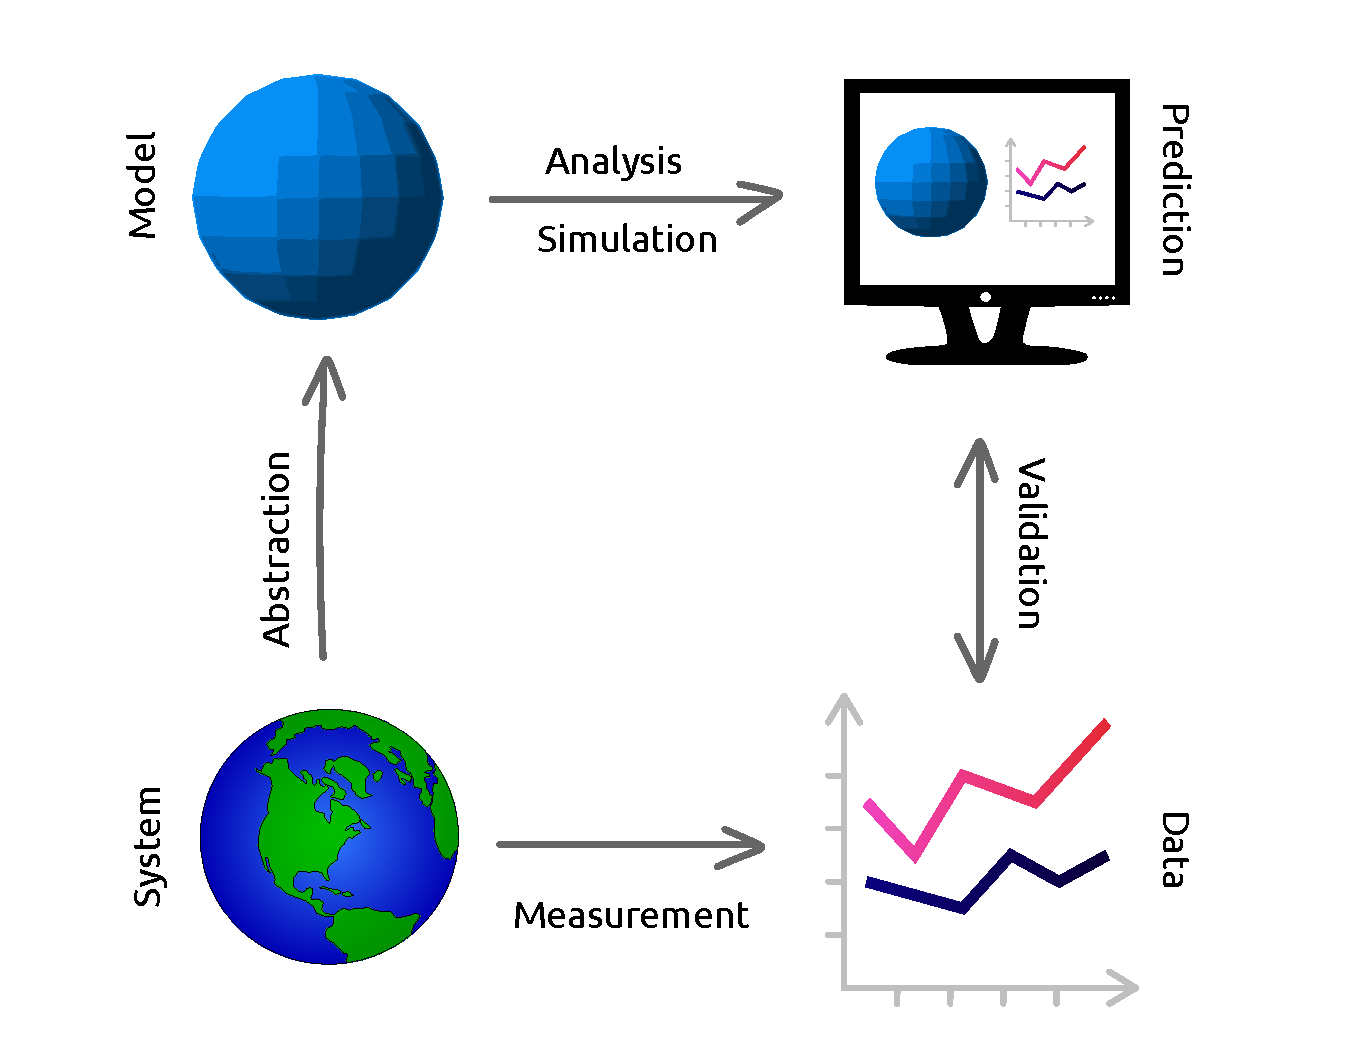
\includegraphics[height=3in]{figs/modeling_framework.pdf}}

Starting in the lower left, the {\bf system} is something in the real world we are interested in.  Often, it is something complicated, so we have to decide which details can be simplified or {\bf abstracted} away.
\index{system}

The result of abstraction is a {\bf model} that includes the features we think are essential.  A model can be represented in the form of diagrams and equations, which can be used for mathematical {\bf analysis}.  It can also be implemented in the form of a computer program, which can run {\bf simulations}.
\index{model}
\index{abstraction}
\index{analysis}

The result of analysis and simulation can be a {\bf prediction} about what the system will do, an {\bf explanation} of why it behaves the way it does, or a {\bf design} intended to achieve a purpose.
\index{prediction}
\index{explanation}
\index{design}

We can {\bf validate} predictions and test designs by taking {\bf measurements} from the real world and comparing the {\bf data} we get with the results from analysis and simulation. 
\index{validation}
\index{data}

This process is almost always iterative: for any physical system, there are many possible models, each one including and excluding different features, or including different levels of detail.  The goal of the modeling process is to find the model best suited to its purpose (prediction, explanation, or design).
\index{iterative modeling}


Sometimes the best model is the most detailed.  If we include more features, the model is more realistic, and we expect its predictions to be more accurate.
\index{realism}

But often a simpler model is better.  If we include only the essential features and leave out the rest, we get models that are easier to work with, and the explanations they provide can be clearer and more compelling.
\index{simplicity}

As an example, suppose someone asked you why the orbit of the Earth is nearly elliptical.  If you model the Earth and Sun as point masses (ignoring their actual size), compute the gravitational force between them using Newton's law of universal gravitation, and compute the resulting orbit using Newton's laws of motion, you can show that the result is an ellipse.
\index{orbit}
\index{ellipse}

Of course, the actual orbit of Earth is not a perfect ellipse, because of the gravitational forces of the Moon, Jupiter, and other objects in the solar system, and because Newton's laws of motion are only approximately true (they don't take into account relativistic effects).
\index{Newton}
\index{relativity}

But adding these features to the model would not improve the explanation; more detail would only be a distraction from the fundamental cause.  However, if the goal is to predict the position of the Earth with great precision, including more details might be necessary.  

So choosing the best model depends on what the model is for.  It is usually a good idea to start with a simple model, even if it is likely to be too simple, and test whether it is good enough for its purpose.  Then you can add features gradually, starting with the ones you expect to be most essential.

Comparing the results of successive models provides a form of {\bf internal validation}, so you can catch conceptual, mathematical, and software errors.  And by adding and removing features, you can tell which ones have the biggest effect on the results, and which can be ignored.
\index{internal validation}
\index{validation!internal}

\section{Can modeling be taught?}

These essential modeling skills --- abstraction, analysis, simulation, and validation --- are central in engineering, natural sciences, social sciences, medicine, and many other fields.  Some students learn these skills implicitly, but in most schools they are not taught explicitly, and students get little practice.  That's the problem this book is meant to address.  

At Olin College, we use this book in a class called Modeling and Simulation, which all students take in their first semester.  My colleagues, John Geddes and Mark Somerville, and I developed this class and taught it for the first time in 2009.

It is based on our belief that modeling should be taught explicitly, early, and throughout the curriculum.  It is also based on our conviction that computation is an essential part of this process.

If students are limited to the mathematical analysis they can do by hand, they are restricted to a small number of simple physical systems, like a projectile moving in a vacuum or a block on a frictionless plane.

And they will only work with bad models; that is, models that are too simple for their purpose.  In nearly every mechanical system, air resistance and friction are essential features; if we ignore them, our predictions will be wrong and our designs won't work.

In most freshman physics classes, students don't make modeling decisions; sometimes they are not even aware of the decisions that have been made for them.  Our goal is to teach, and for students to practice, the entire modeling process.


\section{How much programming do I need?}

If you have never programmed before, you should be able to read this book, understand it, and do the exercises.  I will do my best to explain everything you need to know; in particular, I have chosen carefully the vocabulary I introduce, and I try to define each term the first time it it used.  If you find that I have used a term without defining it, let me know.

If you have programmed before, you will have an easier time getting started, but you might be uncomfortable in some places.  I take an approach to programming you have probably not seen before.

Most programming classes\footnote{Including many I have taught.} have two big problems:

\begin{enumerate}

\item They go ``bottom up", starting with basic language features and gradually adding more powerful tools.  As a result, it takes a long time before students can do anything more interesting than convert Fahrenheit to Celsius.
\index{bottom up}

\item They have no context.  Students learn to program with no particular goal in mind, so the exercises span an incoherent collection of topics, and the projects tend to be unmotivated.

\end{enumerate}

In this book, you learn to program with an immediate goal in mind: writing simulations of physical systems.  And we proceed ``top down", by which I mean we use professional-strength data structures and language features right away.  In particular, we use the following Python {\bf libraries}:
\index{top down}

\begin{itemize}

\item NumPy for basic numerical computation (see \url{http://www.numpy.org/}).\index{NumPy}

\item SciPy for scientific computation (see \url{http://www.scipy.org/}).
\index{SciPy}

\item matplotlib for visualization (see \url{http://matplotlib.org/}).
\index{Matplotlib}

\item pandas for working with data (see \url{http://pandas.pydata.org/}).\index{Pandas}

\item SymPy for symbolic computation, (see \url{http://www.sympy.org}).\index{SymPy}

\item Pint for units like kilograms and meters (see \url{http://pint.readthedocs.io}).\index{Pint}

\item Jupyter for reading, running, and developing code (see \url{http://jupyter.org}).\index{Jupyter}

\end{itemize}

These tools let you work on more interesting programs sooner, but there are some drawbacks: they can be hard to use, and it can be challenging to keep track of which library does what and how they interact.

I have tried to mitigate these problems by providing a library, called \py{modsim}, that makes it easier to get started with these tools, and provides some additional capabilities.
\index{modsim library}

Some features in the \py{modsim} library are like training wheels; at some point you will probably stop using them and start working with the underlying libraries directly.  Other features you might find useful the whole time you are working through the book, or even later.

I encourage you to read the the \py{modsim} library code.  Most of it is not complicated, and I tried to make it readable.  Particularly if you have some programming experience, you might learn something by reverse-engineering my designs.


\section{How much math and science do I need?} 

I assume that you have studied calculus.  You should know what derivatives and integrals are, but that's about all.  In particular, you don't need to know (or remember) much about finding derivatives or integrals of functions analytically.  If you know the derivative of $x^2$ and you can integrate $2x~dx$, that will do it\footnote{And if you noticed that those two questions answer each other, even better.}.
\index{calculus}

More importantly you should understand what those concepts {\em mean};  but if you don't, this book might help you figure it out.

You don't have to know anything about differential equations.

As for science, we will cover topics from a variety of fields, including demography, epidemiology, medicine, thermodynamics, and mechanics. For the most part, I don't assume you know anything about these topics.  In fact, one of the skills you need to do modeling is the ability to learn enough about new fields to develop models and simulations.

When we get to mechanics, I assume you understand the relationship between position, velocity, and acceleration, and that you are familiar with Newton's laws of motion, especially the second law, which is often expressed as $F = ma$ (force equals mass times acceleration).

I think that's everything you need, but if you find that I left something out, please let me know.


\section{Getting started}
\label{code}

To run the examples and work on the exercises in this book, you will need to be able to:

\begin{enumerate}

\item Install Python on your computer, along with the libraries we will use.

\item Copy my files onto your computer.

\item Run Jupyter, which is a tool for running and writing programs, and load a {\bf notebook}, which is a file that contains code and text.

\end{enumerate}

The next three sections provide details for these steps.  I wish there were an easier way to get started; it's regrettable that you have to do so much work before you write your first program.  Be persistent!


\section{Installing Python and the libraries}

You might already have Python installed on your computer, but you might not have the latest version.  To use the code in this book, you need Python 3.6, or later.  Even if you have the latest version, you probably don't have all of the libraries we need.
\index{intalling Python}

You could update Python and install these libraries, but I strongly recommend that you don't go down that road.  I think you will find it easier to use {\bf Anaconda}, which is a free Python distribution that includes all the libraries you need for this book (and lots more).
\index{Anaconda}

Anaconda is available for Linux, macOS, and Windows.  By default, it puts all files in your home directory, so you don't need administrator (root) permission to install it, and if you have a version of Python already, Anaconda will not remove or modify it.

[Detailed instructions coming soon.]



\section{Copying my files}

The code for this book is available from
\url{https://github.com/AllenDowney/ModSimPy}, which is a {\bf Git repository}.  Git is a software tool that helps you keep track of the programs and other files that make up a project.  A collection of files under Git's control is called a repository\footnote{The really cool kids call it a ``repo".}.  GitHub is a hosting service that provides storage for Git repositories and a convenient web interface.
\index{repository}
\index{Git}
\index{GitHub}

There are several ways you can copy the files from my repository to your computer.

If you don't want to use Git at all, you can download my files
in a Zip archive from \url{http://modsimpy.com/zip}.  Then you need a program like WinZip or gzip to unpack the Zip file.

To use Git, you need a {\bf Git client}, which is a program that manages git repositories.  If you have not used Git before, I recommend GitHub Desktop, which is a simple graphical Git client.  You can download it from \url{https://desktop.github.com}.  Currently, GitHub Desktop is not available for Linux.  On Linux, I suggest using the Git command-line client.  Installation instructions are at \url{http://modsimpy.com/git}.

Once you have a Git client, you can use it to copy files from my repository to your computer, which is called {\bf cloning} in Git's vocabulary.  If you are using a Command-line git client, type

\begin{python}
git clone https://github.com/AllenDowney/ModSimPy
\end{python}

You don't need a GitHub account to do this, but you won't be able to write your changes back to GitHub.

If you want to use GitHub to keep track of the code you write while you are using this book, you can make of a copy of my repository on GitHub, which is called {\bf forking}.  If you don't already have a GitHub account, you'll need to create one.  

Use a browser to view the homepage of my repository at \url{https://github.com/AllenDowney/ModSimPy}.   You should see a gray button in the upper right that says {\sf Fork}.  If you press it, GitHub will create a copy of my repository that belongs to you.  Then you can clone your repository like this:

\begin{python}
git clone https://github.com/YourGitHubUserName/ModSimPy
\end{python}

Of course, you should replace \py{YourGitHubUserName} with your GitHub user name.



\section{Running Jupyter}

The code for each chapter, and starter code for the exercises, is in
Jupyter notebooks.  If you have not used Jupyter before, you can read
about it at \url{http://jupyter.org}.
\index{Jupyter}

[Jupyter instructions coming soon.]


\section*{Contributor List}

If you have a suggestion or correction, send it to 
{\tt downey@allendowney.com}.  Or if you are a Git user, send me a pull request!

If I make a change based on your feedback, I will add you to the contributor list, unless you ask to be omitted.
\index{contributors}

If you include at least part of the sentence the error appears in, that makes it easy for me to search.  Page and section numbers are fine, too, but not as easy to work with.  Thanks!

\begin{itemize}

\item I am grateful to John Geddes and Mark Somerville for their early collaboration with me to create Modeling at Simulation, the class at Olin College this book is based on.

\item My early work on this book benefited from conversations with
my amazing colleagues at Olin College, including John Geddes, Alison
Wood, Chris Lee, and Jason Woodard.

\item I am grateful to Lisa Downey and Jason Woodard for their thoughtful and careful copy editing.



% ENDCONTRIB

\end{itemize}



\normalsize

\cleardoublepage

% TABLE OF CONTENTS
\begin{latexonly}

% \tableofcontents

\cleardoublepage

\end{latexonly}

% START THE BOOK
\mainmatter


\chapter{Modeling}
\label{chap01}

The world is a complicated place.  In order to make sense of it, we use {\bf models}, which are generally smaller and simpler than the thing we want to study.  The word ``model" means different things in different contexts, so it is hard to define except by example.
\index{mathematical model}

Some models are actual objects, like a scale model of a car, which has the same shape as the car, but smaller.  Scale models are often useful for testing properties of mechanical systems, like air resistance.

This book is about {\bf mathematical models}, which are ideas, not objects.  If you studied Newton's laws of motion, what you learned is a mathematical model of how objects move in space when forces are applied to them.
\index{Newton}

\section{The falling penny myth}
\label{penny}

Let's see an example of how models are used.  You might have heard that a penny dropped from the top of the Empire State Building would be going so fast when it hit the pavement that it would be embedded in the concrete; or if it hit a person, it would break their skull.
\index{Empire State Building}
\index{penny}
\index{myth}

We can test this myth by making and analyzing a model.  To get started, I'll assume that the effect of air resistance is small.  This will turn out to be a bad assumption, but bear with me.  If air resistance is negligible, the primary force acting on the penny is gravity, which causes the penny to accelerate downward.
\index{air resistance}

If the initial velocity is 0, the velocity after $t$ seconds is $at$, and the height the penny has dropped at $t$ is
%
\[ h = at^2/2 \]
%
Using algebra, we can solve for $t$:
%
\[ t = \sqrt{2h/a} \]
%
Plugging in the acceleration of gravity, $a = \SI{9.8}{\meter\per\second\squared}$ and the height of the Empire State Building, $h=\SI{381}{\meter}$, we get $t = \SI{8.8}{\second}$.  Then computing $v=at$ we get a velocity on impact of $\SI{86}{\meter\per\second}$, which is about 190 miles per hour.  That sounds like it could hurt.

Of course, these results are not exact because the model is based on simplifications.  For example, we assume that gravity is constant.  In fact, the force of gravity is different on different parts of the globe, and gets weaker as you move away from the surface.  But these differences are small, so ignoring them is probably a good choice for this scenario.
\index{gravity}

On the other hand, ignoring air resistance is not a good choice.  Once the penny gets to about \SI{18}{\meter\per\second}, the upward force of air resistance equals the downward force of gravity, so the penny stops accelerating.  After that, it doesn't matter how far the penny falls; it hits the sidewalk (or your head) at about \SI{18}{\meter\per\second}, much less than \SI{86}{\meter\per\second}, as the simple model predicts.

The statistician George Box famously said ``All models are wrong, but some are useful."  He was talking about statistical models, but his wise words apply to all kinds of models.  Our first model, which ignores air resistance, is very wrong, and probably not useful.  The second model is also wrong, but much better, and probably good enough to refute the myth.
\index{Box, George}

The television show {\it Mythbusters} has tested the myth of the falling penny more carefully; you can view the results at \url{http://modsimpy.com/myth}.  Their work is based on a mathematical model of motion, measurements to determine the force of air resistance on a penny, and a physical model of a human head.
\index{Mythbusters}


\section{Computation}

There are (at least) two ways to work with mathematical models, {\bf analysis} and {\bf simulation}.  Analysis often involves algebra and other kinds of symbolic manipulation.  Simulation often involves computers.
\index{analysis}
\index{simulation}

In this book we do some analysis and a lot of simulation; along the way, I discuss the pros and cons of each.  The primary tools we use for simulation are the Python programming language and Jupyter, which is an environment for writing and running programs.

As a first example, I'll show you how I computed the results from the previous section using Python.  You can view this example, and the other code in this chapter, at \url{http://modsimpy.com/chap01}.  For instructions for downloading and running the code, see Section~\ref{code}.

First I'll create a {\bf variable} to represent acceleration.
\index{variable}
\index{value}

\begin{python}
a = 9.8 * meter / second**2
\end{python}

A variable is a name that corresponds to a value.  In this example, the name is \py{a} and the value is the number \py{9.8} multiplied by the units \py{meter / second**2}.  This example demonstrates some of the symbols Python uses to perform mathematical operations:
\index{operator!mathematical}

\begin{tabular}{l|c}
{\bf Operation} & {\bf Symbol} \\ 
\hline 
Addition & \py{+} \\ 
Subtraction & \py{-} \\ 
Multiplication & \py{*} \\ 
Division & \py{/} \\ 
Exponentiation & \py{**}  \\ 
\end{tabular} 

Next, we can compute the time it takes for the penny to drop \SI{381}{\meter}, the height of the Empire State Building.

\begin{python}
h = 381 * meter
t = sqrt(2 * h / a)
\end{python}

These lines create two more variables: \py{h} gets the height of the building in meters; \py{t} gets the time, in seconds, for the penny to fall to the sidewalk.  \py{sqrt} is a {\bf function} that computes square roots.  Python keeps track of units, so the result, \py{t}, has the correct units, seconds.
\index{unit}
\index{function}
\index{sqrt}

Finally, we can compute the velocity of the penny after $t$ seconds:

\begin{python}
v = a * t
\end{python}

The result is about \SI{86}{\meter\per\second}, again with the correct units.

This example demonstrates analysis and computation using Python.  Next we'll see an example of simulation.


\section{Modeling a bike share system}

Imagine a bike share system for students traveling between Olin College and Wellesley College, which are about 3 miles apart in eastern Massachusetts.
\index{Wellesley College}
\index{Olin College}

This example demonstrates the features of Python we'll use to develop computational simulations of real-world systems.  Along the way, I will make decisions about how to model the system.  In the next chapter we'll review these decisions.

Suppose the system contains 12 bikes and two bike racks, one at Olin and one at Wellesley, each with the capacity to hold 12 bikes.
\index{bike share system}

As students arrive, check out a bike, and ride to the other campus,
the number of bikes in each location changes.  In the simulation,
we'll need to keep track of where the bikes are.  To do that, I'll
create a \py{System} object, which is defined in the \py{modsim} library.  
\index{System object}

Before we can use the library, we have to \py{import} it:

\begin{python}
from modsim import *
\end{python}

This line of code is an {\bf import statement} that tells Python
to read the file {\tt modsim.py} and make the functions it defines available.
\index{import statement}

Functions in the \py{modsim.py} library include \py{sqrt}, which we used in the previous section, and \py{System}, which we are using now.  \py{System} creates a \py{System} object, which is a collection of {\bf system variables}.  
\index{system variable}

\begin{python}
bikeshare = System(olin=10, wellesley=2)
\end{python}

In this example, the system variables are \py{olin} and \py{wellesley} and they represent the number of bikes at Olin and Wellesley.  The initial values are 10 and 2, indicating that there are 10 bikes at Olin and 2 at Wellesley.  The \py{System} object created by \py{System} is assigned to a new variable named \py{bikeshare}.
\index{dot operator}
\index{operator!dot}

We can read the variables inside a \py{System} object using the {\bf dot operator}, like this:

\begin{python}
bikeshare.olin
\end{python}

The result is the value 10.  Similarly, for:

\begin{python}
bikeshare.wellesley
\end{python}

The result is 2.  If you forget what variables a system
object has, you can just type the name:

\begin{python}
bikeshare
\end{python}

The result looks like a table with the variable names and their values:

\begin{tabular}{lr}
 & {\bf \sf value} \\ 
\hline 
{\bf \sf olin} & 10 \\ 
{\bf \sf wellesley} & 2 \\ 
\end{tabular} 

The system variables and their values make up the {\bf state} of the system.  We can update the state by assigning new values to
the variables.  For example, if a student moves a bike from Olin
to Wellesley, we can figure out the new values and assign them:
\index{state}

\begin{python}
bikeshare.olin = 9
bikeshare.wellesley = 3
\end{python}

Or we can use {\bf update operators}, \py{-=} and \py{+=} to subtract 1 from \py{olin} and add 1 to \py{wellesley}:
\index{update operator}
\index{operator!update}

\begin{python}
bikeshare.olin -= 1
bikeshare.wellesley += 1
\end{python}

The result is the same either way.


\section{Plotting}

As the state of the system changes, it is often useful to plot the
values of the variables over time.  The \py{modsim} library provides a functions that creates a new figure:
\index{newfig}

\begin{python}
newfig()
\end{python}

In Jupyter, the behavior of this function depends on a command in the
first cell:

\begin{itemize}

\item If you want the figures to appear in the notebook, use

\begin{python}
%matplotlib notebook
\end{python}

\item If you want the figures to appear in separate windows, use

\begin{python}
%matplotlib qt
\end{python}

\end{itemize}

These commands are not actually Python; they are so-called ``magic commands" that control the behavior of Jupyter.
\index{magic command}
\index{plot}

The following lines plot the state of the system:  

\begin{python}
plot(bikeshare.olin, 'rs-')
plot(bikeshare.wellesley, 'bo-')
\end{python}

The \py{plot} function takes two values, called {\bf arguments}:
\index{argument}

\begin{itemize}

\item The first argument is the variable to plot.  In this example, it's a number, but we'll see later that \py{plot} can handle other objects, too.

\item The second argument is a ``style string'' that determines what the plot should look like.  In general, a {\bf string} is a sequence of letters, numbers, and punctuation that appear in quotation marks.  The style string \py{'rs-'} means we want red squares with lines between them; \py{'bo-'} means we want blue circles with
lines.  
\index{style string}
\index{string!style}

\end{itemize}

The plotting functions in the \py{modsim} library are based on Matplotlib, which is a Python {\bf library} for generating
figures.  To learn more about these functions, you can read
the Matplotlib documentation.  For more about style strings, see
\url{http://modsimpy.com/plot}.
\index{Matplotlib}

\section{Defining functions}

So far we have used functions defined in \py{modsim} and other libraries.  Now we're going to define our own functions.
\index{function}
\index{defining functions}

When you are developing code in Jupyter, it is often efficient to
write 1--2 lines in each cell, test them to confirm they do what
you intend, and then use them to define a new function.  For
example, these lines move a bike from Olin to Wellesley:

\begin{python}
bikeshare.olin -= 1
bikeshare.wellesley += 1
\end{python}

Rather than repeat them every time a bike moves, we can define a
new function:

\begin{python}
def bike_to_wellesley():
    bikeshare.olin -= 1
    bikeshare.wellesley += 1
\end{python}

\py{def} is a special word in Python that indicates we are defining a new
function.  The name of the function is \py{bike_to_wellesley}.
The empty parentheses indicate that this function takes no
arguments.  The colon indicates the beginning of an indented
{\bf code block}.
\index{def}
\index{code block}
\index{body}
\index{indentation}

The next two lines are the {\bf body} of the function.  They have
to be indented; by convention, the indentation is 4 spaces.

When you define a function, it has no immediate effect.  The body
of the function doesn't run until you {\bf call} the function.
Here's how to call this function:
\index{call}

\begin{python}
bike_to_wellesley()
\end{python}

When you call this function, it updates the variables of the
{\tt bikeshare} object; you can check by displaying
or plotting the new state.

When you call a function that takes no arguments, you have to
include the empty parentheses.  If you leave them out, like this:
\index{argument}
\index{parentheses}

\begin{python}
bike_to_wellesley
\end{python}

Python looks up the name of the function and displays:

\begin{python}
<function __main__.bike_to_wellesley>
\end{python}

This result indicates that \py{bike_to_wellesley} is a function.  You don't have to know what \py{__main__} means, but if you see something like this, it probably means that you looked up a function but you didn't
actually run it.  So don't forget the parentheses.


\section{Parameters}

Similarly, we can define a function that moves a bike from
Wellesley to Olin:

\begin{python}
def bike_to_olin():
    bikeshare.wellesley -= 1
    bikeshare.olin += 1
\end{python}

And run it like this:

\begin{python}
bike_to_olin()
\end{python}

One benefit of defining functions is that you avoid repeating chunks
of code, which makes programs smaller.  Another benefit is that the
name you give the function documents what it does, which makes programs
more readable.
\index{parameter}

In this example, there is one other benefit that might be even
more important.  Putting these lines in a function makes the program
more reliable because it guarantees that when we decrease the number
of bikes at Olin, we increase the number of bikes at Wellesley.
That way, we guarantee that the bikes in the model are neither created nor destroyed!

However, now we have two functions that are nearly identical except
for a change of sign.  Repeated code makes programs harder to work with, because if we make a change, we have to make it in several places.

We can avoid that by defining a more general function that moves any number of bikes in either direction:

\begin{python}
def move_bike(n):
    bikeshare.olin -= n
    bikeshare.wellesley += n
\end{python}

The name in parentheses, \py{n}, is a {\bf parameter} of the function.
When we run the function, the argument we provide gets assigned to
the parameter.  So if we run \py{move_bike} like this:

\begin{python}
move_bike(1)
\end{python}

It assigns the value of the argument, \py{1}, to the parameter, \py{n}, and then runs the body of the function.  So the effect is the same as:

\begin{python}
n = 1
bikeshare.olin -= n
bikeshare.wellesley += n
\end{python}

Which moves a bike from Olin to Wellesley.  Similarly, if we call
\py{move_bike} like this:

\begin{python}
move_bike(-1)
\end{python}

The effect is the same as:

\begin{python}
n = -1
bikeshare.olin -= n
bikeshare.wellesley += n
\end{python}

Which moves a bike from Wellesley to Olin.  Now that we have
\py{move_bike}, we can rewrite the other two functions to use it: 

\begin{python}
def bike_to_wellesley():
    move_bike(1)
    
def bike_to_olin():
    move_bike(-1)
\end{python}

If you define the same function name more than once, the new definition
replaces the old one.


\section{Print statements}

As you write more complicated programs, it is easy to lose track of what is going on.  One of the most useful tools for debugging is the {\bf print statement}, which displays text in the Jupyter notebook.
\index{print statement}
\index{statement!print}

Normally when Jupyter runs the code in a cell, it displays the value of the last line of code.  For example, if you run:

\begin{python}
bikeshare.olin
bikeshare.wellesley
\end{python}

Jupyter runs both lines of code, but it only displays the value of the second line.

If you want to display more than one value, you can use print statements:

\begin{python}
print(bikeshare.olin)
print(bikeshare.wellesley)
\end{python}

\py{print} is a function, so it takes an argument in parentheses.  It can also take a sequence of arguments separated by commas, like this:

\begin{python}
print(bikeshare.olin, bikeshare.wellesley)
\end{python}

In this example, the two values appear on the same line, separated by a space.

Print statements are also useful for debugging functions.  For example, if you add a print statement to \py{move_bike}, like this:

\begin{python}
def move_bike(n):
    print('Running move_bike with n =', n)
    bikeshare.olin -= n
    bikeshare.wellesley += n
\end{python}

The first argument of \py{print} is a string; the second is the value of \py{n}, which is a number.  Each time you run \py{move_bike}, it displays a message and the value \py{n}.
\index{string}


\section{If statements}

The \py{modsim} library provides a function called \py{flip} that takes
as an argument a probability between 0 and 1:

\begin{python}
flip(0.7)
\end{python}

The result is one of two values: \py{True} with probability 0.7 or \py{False} with probability 0.3.  If you run this function 100 times, you should to get \py{True} about 70 times and \py{False} about 30 times.  But the results are random, so they might differ from these expectations.
\index{flip}
\index{True}
\index{False}

\py{True} and \py{False} are special values defined by Python.  Note
that they are not strings.  There is a difference between \py{True},
which is a special value, and \py{'True'}, which is a string.
\index{string}
\index{boolean}

\py{True} and \py{False} are called {\bf boolean} values because
they are related to Boolean algebra (\url{http://modsimpy.com/boolean}).

We can use boolean values to control the behavior of the program using
an {\bf if statement}:
\index{if statement}
\index{statement!if}

\begin{python}
if flip(0.5):
    print('heads')
\end{python}

If the result from \py{flip} is \py{True}, the program displays the string \py{'heads'}.  Otherwise it does nothing.

The punctuation for if statements is similar to the punctuation for function definitions: the first line has to end with a colon, and the lines inside the if statement have to be indented.
\index{indentation}
\index{else clause}

Optionally, you can add an {\bf else clause} to indicate what should happen if the result is \py{False}:

\begin{python}
if flip(0.5):
    print('heads')
else:
    print('tails')    
\end{python}

Now we can use \py{flip} to simulate the arrival of students who want to borrow a bike.  Suppose we have data from previous observations about how many students arrive at a particular time of day.  If students arrive every 2 minutes, on average, then during any one-minute period, there is a 50\% chance a student will arrive:

\begin{python}
if flip(0.5):
    bike_to_wellesley()
\end{python}

At the same time, there might be an equal probability that a student at Wellesley wants to ride to Olin:

\begin{python}
if flip(0.5):
    bike_to_olin()
\end{python}

We can combine these snippets of code into a function that simulates a {\bf time step}, which is an interval of time, like one minute:
\index{time step}

\begin{python}
def step():
    if flip(0.5):
        bike_to_wellesley()
    
    if flip(0.5):
        bike_to_olin()
\end{python}

Then we can run a time step, and update the plot, like this:

\begin{python}
step()
plot_state()
\end{python}

In reality, the probability of an arrival will vary over the course of a day, and might be higher or lower, at any point in time, at Olin or Wellesley.  So instead of putting the constant value 0.5 in \py{step} we can replace it with a parameter, like this:
\index{probability}

\begin{python}
def step(p1, p2):
    if flip(p1):
        bike_to_wellesley()
    
    if flip(p2):
        bike_to_olin()
\end{python}

Now when you call \py{step}, you have to provide two arguments:

\begin{python}
step(0.4, 0.2)
\end{python}

The arguments you provide, \py{0.4} and \py{0.2}, get assigned to the parameters, \py{p1} and \py{p2}, in order.  So running this function has the same effect as:

\begin{python}
p1 = 0.4
p2 = 0.2

if flip(p1):
    bike_to_wellesley()
    
if flip(p2):
    bike_to_olin()
\end{python}



\section{Optional parameters}

When you add parameters to a function, you can provide {\bf default values}, like this:
\index{parameter!optional}
\index{optional parameter}

\begin{python}
def step(p1=0.5, p2=0.5):
    if flip(p1):
        bike_to_wellesley()
    
    if flip(p2):
        bike_to_olin()
\end{python}

Because they have default values, these parameters are optional; if you run \py{step} with no arguments, and don't forget the parentheses, like this:

\begin{python}
step()
\end{python}

The parameters get the default values, so \py{p1} and \py{p2} are both \py{0.5}.  If you provide one argument, like this:

\begin{python}
step(0.4)
\end{python}

The value you provide {\bf overrides} the default value of \py{p1}, but \py{p2} still gets the default.  If you provide two arguments, it overrides both.
\index{override}

\begin{python}
step(0.4, 0.2)
\end{python}

If you want to override \py{p2} only, and accept the default for \py{p1}, you have to provide the name of the parameter explicitly:

\begin{python}
step(p2=0.2)
\end{python}

It is always legal to provide parameter names along with the arguments:

\begin{python}
step(p1=0.4, p2=0.2)
\end{python}

Providing parameters names makes programs more readable and less error-prone, because you don't have to worry about the order of the arguments.  For example, if you reverse the order, it still assigns the right value to each parameter:

\begin{python}
step(p2=0.2, p1=0.4)
\end{python}


\section{For loops}
\label{forloop}

At some point you will get sick of running cells over and over. Fortunately, there is an easy way to repeat a chunk of code, the {\bf for loop}.  Here's an example:
\index{for loop}
\index{loop}

\begin{python}
for i in range(4):
    bike_to_wellesley()
    plot_state()
\end{python}

The punctuation here should look familiar; the first line ends with a colon, and the lines inside the for loop are indented.  The other elements of the for loop are:
\index{range}

\begin{itemize}

\item The words \py{for} and \py{in} are special words we have to use in a for loop.  

\item \py{range} is a Python function we're using here to control the number of times the loop runs.
\index{range}

\item \py{i} is a {\bf loop variable} that gets created when the for loop runs.  In this example we don't actually use \py{i}; we will see examples later where we use the loop variable inside the loop.
\index{loop variable}

\end{itemize}

When this loop runs, it runs the statements inside the loop four times, 
which moves one bike at a time from Olin to Wellesley, and plots the updated state of the system after each move.


\section{Debugging}

The goal of this chapter is to give you the minimal set of tools to get you started.  At this point, you know enough to write simple simulations of systems like the Olin--Wellesley bikeshare.  Along with each chapter, I provide a Jupyter notebook that contains the code from the chapter, so you can run it, see how it works, modify it, and see how it breaks.
\index{debugging}

When something goes wrong, Python provides error messages with information about the problem.  This information can help with debugging, but error messages are often hard to understand.
\index{error message}

When you are learning a programming language, it is a good idea to make as many mistakes as you can, deliberately, so you can see what happens.  You will start to understand the error messages better, which helps when you make errors accidentally.



\chapter{Simulation}

To paraphrase two Georges, ``All models are wrong, but some models are more wrong than others."  In this chapter, I demonstrate the process we use to make models less wrong.
\index{Box, George}
\index{Orwell, George}

As an example, we'll review the bikeshare model from the previous chapter, consider its strengths and weaknesses, and gradually improve it.  We'll also see ways to use the model to understand the behavior of the system and evaluate designed intended to make it work better.
\index{bikeshare}

You can view the code for this chapter at \url{http://modsimpy.com/chap02}.  For instructions for downloading and running the code, see Section~\ref{code}.


\section{Iterative modeling}

The model we have so far is simple, but it is based on unrealistic assumptions.  Before you go on, take a minute to review the code from the previous chapter, which you can view at \url{http://modsimpy.com/chap01}.  This code represents a model of the bikeshare system.  What assumptions is it based on?  Make a list of ways this model might be unrealistic; that is, what are the differences between the model and the real world?
\index{iterative modeling}

Here are some of the differences on my list:

\begin{itemize}

\item In the model, a student is equally likely to arrive during any one-minute period.  In reality, this probability varies depending on time of day, day of the week, etc.
\index{probability}

\item The model does not account for travel time from one bike station to another.

\item The model does not check whether a bike is available, so it's possible for the number of bikes to be negative (as you might have noticed in some of your simulations).

\end{itemize}

Some of these modeling decisions are better than others.  For example, the first assumption might be reasonable if we simulate the system for a short period of time, like one hour.

The second assumption is not very realistic, but it might not affect the results very much, depending on what we use the model for.
\index{realism}

On the other hand, the third assumption seems problematic, and it is relatively easy to fix.  In Section~\ref{negativebikes}, we will.

This process, starting with a simple model, identifying the most important problems, and making gradual improvements, is called {\bf iterative modeling}.

For any physical system, there are many possible models, based on different assumptions and simplifications.  It often takes several iterations to develop a model that is good enough for the intended purpose, but no more complicated than necessary.


\section{More than one System object}

Before we go on, I want to make a few changes to the code from the previous chapter.  First, I will generalize the functions we wrote so they take a \py{System} object as a parameter.  Then, we will make the code more readable by adding documentation.
\index{parameter}

Here are two functions from the previous chapter, \py{move_bike} and \py{plot_state}:

\begin{python}
def move_bike(n):
    bikeshare.olin -= n
    bikeshare.wellesley += n

def plot_state():
    plot(bikeshare.olin, 'rs-', label='Olin')
    plot(bikeshare.wellesley, 'bo-', label='Wellesley')
\end{python}

One problem with these functions is that they always use \py{bikeshare}, which is a \py{System} object.  As long as there is only one \py{System} object, that's fine, but these functions would be more flexible if they took a \py{System} object as a parameter.  Here's what that looks like:
\index{System object}

\begin{python}
def move_bike(system, n):
    system.olin -= n
    system.wellesley += n

def plot_state(system):
    plot(system.olin, 'rs-', label='Olin')
    plot(system.wellesley, 'bo-', label='Wellesley')
\end{python}

The name of the parameter is \py{system} rather than \py{bikeshare} as a reminder that the value of \py{system} could be any \py{System} object, not just \py{bikeshare}.

Now I can create as many \py{System} objects as I want:

\begin{python}
bikeshare1 = System(olin=10, wellesley=2)
bikeshare2 = System(olin=2, wellesley=10)
\end{python}

And update them independently:

\begin{python}
bike_to_olin(bikeshare1)
bike_to_wellesley(bikeshare2)
\end{python}

Changes in \py{bikeshare1} do not affect \py{bikeshare2}, and vice versa.  This behavior will be useful later in the chapter when we create a series of \py{System} objects to simulate different scenarios.


\section{Documentation}

Another problem with the code we have so far is that it contains no {\bf documentation}.  Documentation is text we add to programs to help other programmers read and understand them.  It has no effect on the program when it runs.
\index{documentation}
\index{docstring}
\index{comment}

There are two forms of documentation, {\bf docstrings} and {\bf comments}.   
 A docstring is a string in triple-quotes that appears at the beginning of a function, like this:

\begin{python}
def run_steps(system, num_steps=1, p1=0.5, p2=0.5):
    """Simulate the given number of time steps.
    
    system: bikeshare System object
    num_steps: number of time steps
    p1: probability of an Olin->Wellesley customer arrival
    p2: probability of a Wellesley->Olin customer arrival
    """
    for i in range(num_steps):
        step(system, p1, p2)
        plot_state(system)
\end{python}

Docstrings follow a conventional format:

\begin{itemize}

\item The first line is a single sentence that describes what the function does.

\item The following lines explain what each of the parameters are.

\end{itemize}

A function's docstring should include the information someone needs to know to {\em use} the function; it should not include details about how the function works.  That's what comments are for.

A comment is a line of text that begins with a hash symbol, \py{#}.  It usually appears inside a function to explain something that would not be obvious to someone reading the program.
\index{hash symbol}

For example, here is a version of \py{move_bike} with a docstring and a comment.

\begin{python}
def move_bike(system, n):
    """Move a bike.
    
    system: bikeshare System object
    n: +1 to move from Olin to Wellesley or
       -1 to move from Wellesley to Olin
    """
    # Because we decrease one system variable by n
    # and increase the other by n, the total number
    # of bikes is unchanged.
    system.olin -= n
    system.wellesley += n
\end{python}

At this point we have more documentation than code, which is not unusual for short functions.


\section{Negative bikes}
\label{negativebikes}

The changes we've made so far improve the quality of the code, but we haven't done anything to improve the quality of the model yet.   Let's do that now.
\index{code quality}

Currently the code does not check whether a bike is available when a customer arrives, so the number of bikes at a location can be negative.  That's not very realistic.  Here's an updated version of \py{move_bike} that fixes the problem:

\begin{python}
def move_bike(system, n):
    # make sure the number of bikes won't go negative
    olin_temp = system.olin - n
    if olin_temp < 0:
        return
    
    wellesley_temp = system.wellesley + n
    if wellesley_temp < 0:
        return
    
    # update the system
    system.olin = olin_temp
    system.wellesley = wellesley_temp
\end{python}

The comments explain the two sections of the function: the first checks to make sure a bike is available; the second updates the state.

The first line creates a variable named \py{olin_temp} that gets the number of bikes that {\em would} be at Olin if \py{n} bikes were moved.  I added the suffix \py{_temp} to the name to indicate that I am using it as a {\bf temporary variable}.
\index{temporary variable}
\index{variable!temporary}

\py{move_bike} uses the less-than operator, \py{<}, to compare \py{olin_temp} to \py{0}.  The result of this operator is a boolean.  If it's \py{True}, that means \py{olin_temp} is negative, which means that there are not enough bikes.
\index{operator}
\index{return statement}
\index{statement!return}

In that case I use a {\bf return statement}, which causes the function to end immediately, without running the rest of the statements.  So if there are not enough bikes at Olin, we ``return" from \py{move_bike} without changing the state.  We do the same if there are not enough bikes at Wellesley.

If both of these tests pass, we run the last two lines, which assigns the values from the temporary variables to the corresponding system variables.

Because \py{olin_temp} and \py{wellesley_temp} are created inside a function, they are {\bf local variables}, which means they only exist inside the function.  At the end of the function, they disappear, and you cannot read or write them from anywhere else in the program.
\index{local variables}
\index{variables!local}

In contrast, the system variables \py{olin} and \py{wellesley} belong to \py{system}, the \py{System} object that was passed to this function as a parameter.  When we change system variables inside a function, those changes are visible in other parts of the program.

This version of \py{move_bike} makes sure we never have negative bikes at either station.  But what about \py{bike_to_wellesley} and \py{bike_to_olin}; do we have to update them, too?  Here they are:

\begin{python}
def bike_to_wellesley(system):
    move_bike(system, 1)
    
def bike_to_olin(system):
    move_bike(system, -1)
\end{python}

Because these functions use \py{move_bike}, they take advantage of the new feature automatically.  We don't have to update them.


\section{Comparison operators}

In the previous section, we used the less-than operator to compare two values.  For completeness, here are the other {\bf comparison operators}:
\index{comparison operator}
\index{operator!comparison}

\begin{tabular}{l|c}
{\bf Operation} & {\bf Symbol} \\ 
\hline 
Less than & \py{<} \\ 
Greater than & \py{>} \\
Less than or equal & \py{<=}  \\ 
Greater than or equal & \py{>=} \\ 
Equal & \py{==} \\ 
Not equal & \py{!=} \\ 
\end{tabular} 

The equals operator, \py{==}, compares two values and returns \py{True} if they are equal and \py{False} otherwise.  It is easy to confuse with the {\bf assignment operator}, \py{=}, which assigns a value to a variable.  For example, the following statement uses the assignment operator, which creates \py{x} if it doesn't already exist and gives it the value \py{5}
\index{equality}
\index{assignment operator}
\index{operator!assignment}

\begin{python}
x = 5
\end{python}

On the other hand, the following statement checks whether \py{x} is \py{5} and returns \py{True} or \py{False}.  It does not create \py{x} or change its value.  

\begin{python}
x == 5
\end{python}

You can use the equals operator in an if statement, like this:
\index{if statement}
\index{statement!if}

\begin{python}
if x == 5:
    print('yes, x is 5')
\end{python}

If you make a mistake and use \py{=} in the first line of an \py{if} statement, like this:

\begin{python}
if x = 5:
    print('yes, x is 5')
\end{python}

That's a {\bf syntax error}, which means that the structure of the program is invalid.  Python will print an error message and the program won't run.
\index{syntax error}
\index{error!syntax}

\section{Metrics}

Getting back to the bike share system, at this point we have the ability to simulate the behavior of the system.  Since the arrival of customers is random, the state of the system is different each time we run a simulation.  Models like this are called {\bf stochastic}; models that do the same thing every time they run are {\bf deterministic}.
\index{stochastic}
\index{deterministic}

Suppose we want to use our model to predict how well the bike share system will work, or to design a system that works better.  First, we have to decide what we mean by ``how well" and ``better".

From the customer's point of view, we might like to know the probability of finding an available bike.  From the system-owner's point of view, we might want to minimize the number of customers who don't get a bike when they want one, or maximize the number of bikes in use.  Statistics like these that are intended to quantify how well the system works are called {\bf metrics}.
\index{metric}

As a simple example, let's measure the number of unhappy customers.  Here's a version of \py{move_bike} that keeps track of the number of customers who arrive at a station with no bikes:

\begin{python}
def move_bike(system, n):
    olin_temp = system.olin - n
    if olin_temp < 0:
        system.olin_empty += 1
        return
    
    wellesley_temp = system.wellesley + n
    if wellesley_temp < 0:
        system.wellesley_empty += 1
        return
    
    system.olin = olin_temp
    system.wellesley = wellesley_temp
\end{python}

Inside \py{move_bike}, we update the values of \py{olin_empty}, which is the number of times a customer finds the Olin station empty, and \py{wellesley_empty}, which is the number of unhappy customers at Wellesley.

That will only work if we initialize \py{olin_empty} and \py{wellesley_empty} when we create the \py{System} object, like this:

\begin{python}
bikeshare = System(olin=10, wellesley=2, 
                   olin_empty=0, wellesley_empty=0)
\end{python}

Now we can run a simulation like this:

\begin{python}
run_steps(bikeshare, 60, 0.4, 0.2)
\end{python}

And then check the metrics:

\begin{python}
print(bikeshare.olin_empty, bikeshare.wellesley_empty)
\end{python}

Because the simulation is stochastic, the results are different each time it runs.


\section{Functions that return values}

We have used several functions that return values; for example, when you run \py{sqrt}, it returns a number you can assign to a variable.
\index{return value}

\begin{python}
t = sqrt(2 * h / a)
\end{python}

When you run \py{System}, it returns a new \py{System} object:
 
\begin{python}
bikeshare = System(olin=10, wellesley=2)
\end{python}

Not all functions have return values.  For example, when you run \py{plot}, it adds a point to the current graph, but it doesn't return a value.  The functions we wrote so far are like \py{plot}; they have an effect, like changing the state of the system, but they don't return values.

To write functions that return values, we can use a second form of the \py{return} statement, like this:
\index{return statement}
\index{statement!return}

\begin{python}
def add_five(x):
    return x + 5
\end{python}

\py{add_five} takes a parameter, \py{x}, which could be any number.  It computes \py{x + 5} and returns the result.  So if we run it like this, the result is \py{8}:

\begin{python}
add_five(3)
\end{python}

As a more useful example, here's a new function that creates a \py{System} object, runs a simulation, and then returns the \py{System} object as a result:

\begin{python}
def run_simulation():
    system = System(olin=10, wellesley=2, 
                    olin_empty=0, wellesley_empty=0)
    run_steps(system, 60, 0.4, 0.2, plot=False)
    return system
\end{python}

If we call \py{run_simulation} like this:

\begin{python}
system = run_simulation()
\end{python}

It assigns to \py{system} a new \py{System} object, which we can use to check the metrics we are interested in:

\begin{python}
print(system.olin_empty, system.wellesley_empty)
\end{python}


\section{Two kinds of parameters}

This version of \py{run_simulation} always starts with the same initial condition, 10 bikes at Olin and 2 bikes at Wellesley, and the same values of \py{p1}, \py{p2}, and \py{num_steps}.  Taken together, these five values are the {\bf parameters of the model}, which are values that determine the behavior of the model.
\index{parameter!of a model}
\index{parameter!of a function}

It is easy to get the parameters of a model confused with the parameters of a function.  They are closely related ideas; in fact, it is common for the parameters of the model to appear as parameters in functions.  For example, we can write a more general version of \py{run_simulation} that takes \py{p1} and \py{p2} as function parameters:

\begin{python}
def run_simulation(p1=0.4, p2=0.2):
    bikeshare = System(olin=10, wellesley=2, 
                  olin_empty=0, wellesley_empty=0)
    run_steps(bikeshare, 60, p1, p2, plot=False)
    return bikeshare
\end{python}

Now we can run it with different arrival rates, like this:

\begin{python}
system = run_simulation(p1=0.6, p2=0.3)
\end{python}

Then we can see how the metrics, like the number of unhappy customers, depend on the parameters of the model.  But before we do that, we need a new version of a for loop.
\index{metric}

\section{Loops and arrays}
\label{array}

In Section~\ref{forloop}, we saw a loop like this:

\begin{python}
for i in range(4):
    bike_to_wellesley()
    plot_state()
\end{python}

The loop variable, \py{i}, gets created when the loop runs, but it is not used for anything.  Now here's a loop that actually uses the loop variable:
\index{loop}
\index{loop variable}
\index{variable!loop}

\begin{python}
p1_array = linspace(start=0, stop=1, num=5)

for p1 in p1_array:
    print(p1)
\end{python}

\py{linspace} is a function defined in the \py{modsim} library.  It takes three arguments, \py{start}, \py{stop}, and \py{num}.  In this example, it creates a sequence of \py{5} equally-spaced numbers, starting at \py{0} and ending at \py{1}. 
\index{linspace}
\index{NumPy}
\index{array}

The result is a NumPy {\bf array}, which is a new kind of object we have not seen before.  An array is a container for a sequence of numbers. 

In the for loop, the values from the array are assigned to the loop variable one a time.  When this loop runs, it

\begin{enumerate}

\item Gets the first value from the array and assigns it to \py{p1}.

\item Runs the body of the loop, which prints \py{p1}.

\item Gets the next value from the array and assigns it to \py{p1}.

\item Runs the body of the loop, which prints \py{p1}.

\end{enumerate}

And so on, until it gets to the end of the range.  The result is:

\begin{result}
0.0
0.25
0.5
0.75
1.0
\end{result}

This will come in handy in the next section.


\section{Sweeping parameters}

If we know the actual values of parameters like \py{p1} and \py{p2}, we can use them to make specific predictions, like how many bikes will be at Olin after one hour.  If that's the goal, we'll probably have to collect data and estimate \py{p1} and \py{p2}.
\index{prediction}
\index{explanation}

But prediction is not the only goal; models like this are also used to explain why systems behave as they do and to evaluate alternative designs.  For example, if we observe the system and notice that we often run out of bikes at a particular time, we could use the model to figure out why that happens.  And if we are considering adding more bikes, or another station, we could evaluate the effect of various ``what if" scenarios.
\index{what if scenario}

As an example, suppose we have enough data to estimate that \py{p2} is about \py{0.2}, but we don't have any information about \py{p1}.  We could run simulations with a range of values for \py{p1} and see how the results vary.  This process is called {\bf sweeping} a parameter, in the sense that the value of the parameter ``sweeps" through a range of possible values.
\index{sweep}
\index{parameter sweep}

Now that we know about loops and arrays, we can use them like this:

\begin{python}
p1_array = linspace(0, 1, 11)

for p1 in p1_array:
    system = run_simulation(p1=p1)
    print(p1, system.olin_empty)
\end{python}

Each time through the loop, we run a simulation with a the given value of \py{p1} and the default value of \py{p2}.  Then we print \py{p1} and the number of unhappy customers at Olin.

To visualize the results, we can run the same loop, replacing \py{print} with \py{plot}:

\begin{python}
newfig()
for p1 in p1_array:
    system = run_simulation(p1=p1)
    plot(p1, system.olin_empty, 'rs', label='olin')
\end{python}

When you run the notebook for this chapter, you will see the results and have a chance to try additional experiments.


\section{Debugging}

When you start writing programs that are more than a few lines, you
might find yourself spending more and more time debugging.  The more
code you write before you start debugging, the harder it is to find
the problem.
\index{debugging}
\index{incremental development}

{\bf Incremental development} is a way of programming that tries
to minimize the pain of debugging.  The fundamental steps are:

\begin{enumerate}

\item Always start with a working program.  If you have an
example from a book, or a program you wrote that is similar to
what you are working on, start with that.  Otherwise, start with
something you {\em know} is correct, like {\tt x=5}.  Run the program
and confirm that it does what you expect.

\item Make one small, testable change at a time.  A ``testable''
change is one that displays something, or has some
other effect, that you can check.  Ideally, you should know what
the correct answer is, or be able to check it by performing another
computation. 
\index{testable change}

\item Run the program and see if the change worked.  If so, go back
to Step 2.  If not, you will have to do some debugging, but if the
change you made was small, it shouldn't take long to find the problem.

\end{enumerate}

When this process works, your changes usually work the first time, or if they don't, the problem is obvious.  In practice, there are two problems with incremental development:

\begin{itemize}

\item Sometimes you have to write extra code to generate visible output that you can check.  This extra code is called {\bf scaffolding} because you use it to build the program and then remove it when you are done.  That might seem like a waste, but time you spend on scaffolding is almost always time you save on debugging.
\index{scaffolding}

\item When you are getting started, it might not be obvious how to
choose the steps that get from {\tt x=5} to the program you are trying
to write.  You will see more examples of this process as we go along, and you will get better with experience.

\end{itemize}

If you find yourself writing more than a few lines of code before you start testing, and you are spending a lot of time debugging, try incremental development.


\chapter{Explanation}

In 1968 Paul Erlich published {\it The Population Bomb}, in which he predicted that world population would grow quickly during the 1970s, that agricultural production could not keep up, and that mass starvation in the next two decades was inevitable (see \url{http://modsimpy.com/popbomb}).  As someone who grew up during those decades, I am happy to report that those predictions were wrong.  
\index{Erlich, Paul}
\index{Population Bomb}

But world population growth is still a topic of concern, and it is an open question how many people the earth can sustain while maintaining and improving our quality of life.
\index{world population}
\index{population}

In this chapter and the next, we use tools from the previous chapters to explain world population growth since 1950 and generate predictions for the next 50--100 years.
\index{prediction}

You can view the code for this chapter at \url{http://modsimpy.com/chap03}.  For instructions for downloading and running the code, see Section~\ref{code}.


\section{World population data}
\label{worldpopdata}

The Wikipedia article  \url{http://modsimpy.com/worldpop}
contains tables with estimates of world population from prehistory to the present, and projections for the future.
\index{Wikipedia}

To work with this data in Python, we will use functions from Pandas, which is a library that provides functions for working with data.  It also defines two objects we will use extensively, \py{Series} and \py{DataFrame}.
\index{data}
\index{Pandas}
\index{Series}
\index{DataFrame}

The Pandas function we'll use is \py{read_html}, which can read a web page and extract data from any tables it contains.  Before we can use it, we have to import it.  You have already seen this import statement:
\index{\py{read_html}}
\index{import statement}
\index{statement!import}

\begin{python}
from modsim import *
\end{python}

which imports all functions from the \py{modsim} library.  To import \py{read_html}, the statement we need is:

\begin{python}
from pandas import read_html
\end{python}

Now we can use it like this:

\begin{python}
filename = 'data/World_population_estimates.html'
tables = read_html(filename,
                   header=0, 
                   index_col=0,
                   decimal='M')
\end{python}

The arguments are:
\index{argument}

\begin{itemize}

\item \py{filename}: The name of the file (including the directory it's in) as a string.  This argument can also be a URL starting with \py{http}.

\item \py{header}: Indicates which row of each table should be considered the header, that is, the row that contains the column headings.  In this case it is the first row, which is numbered 0.

\item \py{index_col}: Indicates which column of each table should be considered the index, that is, the labels that identify the rows.  In this case it is the first column, which contains the years.

\item \py{decimal}: Normally this argument is used to indicate which character should be considered a decimal point, since some conventions use a period and some use a comma.  In this case I am abusing the feature by treating \py{M} as a decimal point, which allows some of the estimates, which are expressed in millions, to be read as numbers.

\end{itemize}

The result, which is assigned to \py{tables}, is a sequence that contains one \py{DataFrame} for each table.  A \py{DataFrame} is an object that represents tabular data and provides functions for accessing and manipulating it.
\index{DataFrame}
\index{sequence}

To select one of the \py{DataFrame}s in \py{tables}, we can use the bracket operator like this:

\begin{python}
table2 = tables[2]
\end{python}

The number in brackets indicates which \py{DataFrame} we want, starting from 0.  So this line selects the third table, which contains population estimates from 1950 to 2016.
\index{bracket operator}
\index{operator!bracket}

We can display the first few lines like this:

\begin{python}
table2.head()
\end{python}

The headings at the tops of the columns are long strings, which makes them hard to work.  We can replace them with shorter strings like this:
\index{string}
\index{columns}

\begin{python}
table2.columns = ['census', 'prb', 'un', 'maddison', 
                  'hyde', 'tanton', 'biraben', 'mj', 
                  'thomlinson', 'durand', 'clark']
\end{python}


\section{Series}
\label{series}

Now we can select a column from the \py{DataFrame} using the dot operator, like selecting a system variable from a \py{System} object:
\index{dot operator}
\index{operator!dot}

\begin{python}
census = table2.census
\end{python}

The result is a \py{Series}, which is another object defined by the Pandas library.  Each \py{Series} object contains variables called \py{index} and \py{values}.  In this example, the \py{index} is a sequence of years, from 1950 to 2015; \py{values} is a sequence of population estimates.
\index{series}
\index{index}
\index{values}

\py{values} is an array like the ones we saw in Section~\ref{array}.  \py{index} is an \py{Int64Index}, which is yet another object defined by Pandas, but in all ways we care about for now, it behaves like an array.
\index{array}
\index{Int64Index}

\py{plot} knows how to work with \py{Series} objects, so we can plot the estimates like this:
\index{plot}

\begin{python}
def plot_estimates():
    un = table2.un / 1e9
    census = table2.census / 1e9
    
    plot(census, ':', color='darkblue', label='US Census')
    plot(un, '--', color='green', label='UN DESA')
\end{python}

The first two lines select the estimates generated by the United Nations Department of Economic and Social Affairs (UN DESA) and the United States Census Bureau.
\index{United Nations}
\index{United States Census Bureau}

At the same time we divide by one billion, in order to display the estimates in terms of billions.  The number \py{1e9} is a shorter (and less error-prone) way to write \py{1000000000} or one billion.  When we divide a \py{Series} by a number, it divides all of the elements of the \py{Series}.

The next two lines plot the \py{Series} objects.  The strings \py{':'} and \py{'--'} indicate dotted and dashed lines.  The \py{color} argument can be any of the color strings described at \url{http://modsimpy.com/color}.  The \py{label} argument provides the string that appears in the legend.
\index{color}
\index{label}
\index{legend}

\begin{figure}
\centerline{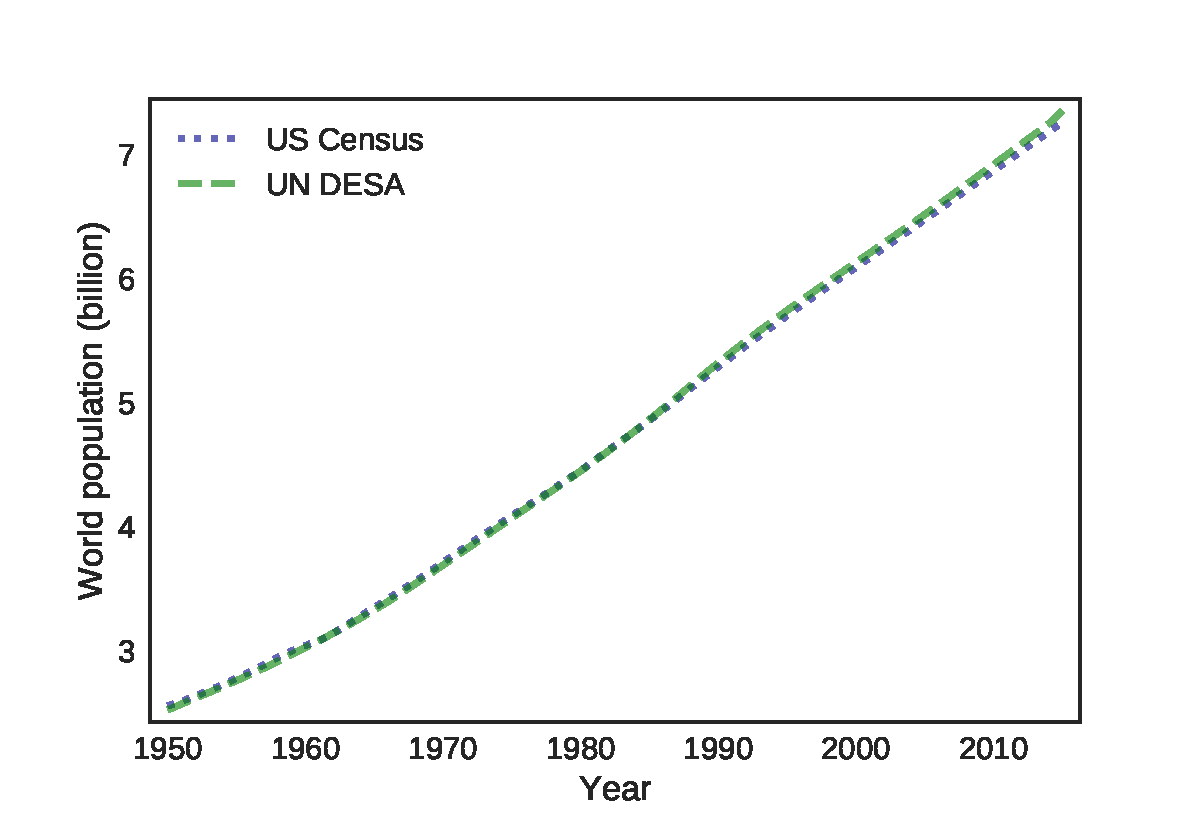
\includegraphics[height=3in]{figs/chap03-fig01.pdf}}
\caption{Estimates of world population, 1950--2015.}
\label{chap03-fig01}
\end{figure}

Figure~\ref{chap03-fig01} shows the result.  The lines overlap almost completely; for most dates the difference between the two estimates is less than 1\%.


\section{Constant growth model}

Suppose we want to predict world population growth over the next 50 or 100 years.  We can do that by developing a model that describes how population grows, fitting the model to the data we have so far, and then using the model to generate predictions.
\index{constant growth}

In the next few sections I demonstrate this process starting with simple models, which turn out to be unrealistic, and gradually improving them.
\index{iterative modeling}

Although there is some curvature in the plotted estimates, it looks like world population growth has been close to linear since 1960 or so.  As a starting place, we'll build a model with constant growth.

To fit the model to the data, we'll compute the average annual growth from 1950 to 2015.  Since the UN and Census data are so close, I'll use the Census data, again in terms of billions:

\begin{python}
census = table2.census / 1e9
\end{python}

We can select a value from a \py{Series} using the bracket operator:
\index{bracket operator}
\index{operator!bracket}

\begin{python}
census[1950]
\end{python}

So we can get the total growth during the interval like this:

\begin{python}
total_growth = census[2015] - census[1950]
\end{python}

The values 2015 and 1950 are part of the data, so it would be better not to make them part of the program.  Putting values like these in the program is called {\bf hard coding}; it is considered bad practice because if the data changes in the future, we have to modify the program (see \url{http://modsimpy.com/hardcode}).
\index{hard coding}

We can get the first and last year from the index like this:

\begin{python}
first_year = census.index[0]
last_year = census.index[-1]
\end{python}

In brackets, \py{0} selects the first element from \py{census.index}, and \py{-1} selects the last element.  Now we can compute \py{total_growth} and \py{annual_growth}:

\begin{python}
total_growth = census[last_year] - census[first_year]
elapsed_time = last_year - first_year
annual_growth = total_growth / elapsed_time
\end{python}

The next step is to use this estimate to simulate population growth since 1950.

\section{Simulation}

The result from the simulation is a time series, which is a sequence of dates or times and an associated series of values (see \url{http://modsimpy.com/timeser}).  In this case, we have a sequence of year and an associated sequence of population estimates with associated year.
\index{time series}
\index{TimeSeries object}
\index{simulation}

To represent a time series, we'll use a \py{TimeSeries} object:

\begin{python}
results = TimeSeries()
\end{python}

\py{TimeSeries}, which is defined by \py{modsim}, is a specialized version of \py{Series}, which is defined by Pandas. 
\index{Pandas}

We can set the first value in the new \py{TimeSeries} by copying the first value from \py{census} (we'll get rid of the hard-coded dates soon):

\begin{python}
results[1950] = census[1950]
\end{python}

Then we can set the rest of the values by simulating annual growth:

\begin{python}
for t in linrange(1950, 2015):
    results[t+1] = results[t] + annual_growth
\end{python}

\py{linrange} is defined in the \py{modsim} library.  It is similar to \py{linspace}, but instead of taking parameters \py{start}, \py{stop}, and \py{num}, it takes \py{start}, \py{stop}, and \py{step}.
\index{linrange}
\index{linspace}

It returns a NumPy array of values from \py{start} to \py{stop}, where \py{step} is the difference between successive values.  The default value of \py{step} is 1.

This function works best if the space between \py{start} and \py{stop} is divisible by \py{step}; otherwise the results might be surprising.

By default, the last value in the array is \py{stop} (at least approximately).  If you provide the argument \py{endpoint=False}, the last value in the array is \py{stop-step}. 

In this example, the result from \py{linrange} is an array of values from \py{1950} to \py{2015} (including both).  
\index{array}

Each time through the loop, the loop variable \py{t} gets the next value from the array.  Inside the loop, we compute the population for each year by adding the population for the previous year and \py{annual_growth}.
\index{loop}
\index{loop variable}

\begin{figure}
\centerline{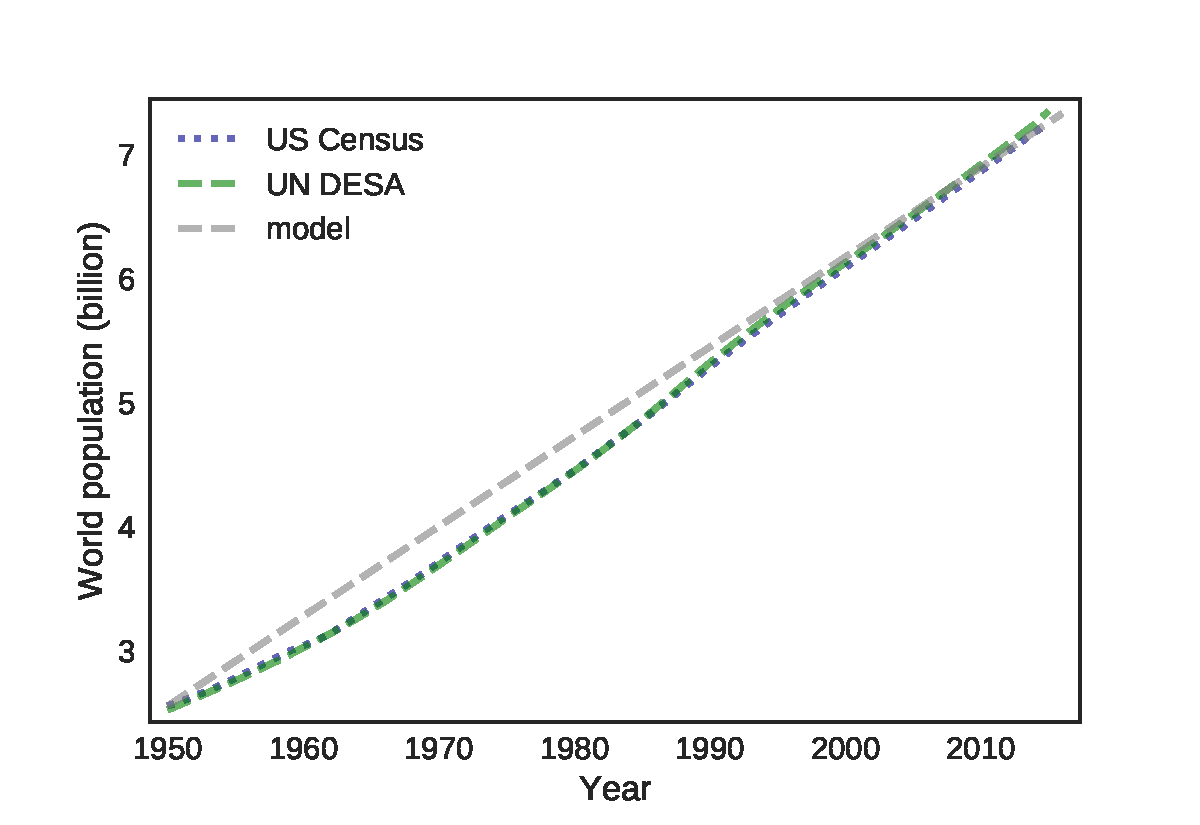
\includegraphics[height=3in]{figs/chap03-fig02.pdf}}
\caption{Estimates of world population, 1950--2015, and a constant growth model.}
\label{chap03-fig02}
\end{figure}

Figure~\ref{chap03-fig02} shows the result. The model does not fit the data particularly well from 1950 to 1990, but after that, it's pretty good.  Nevertheless, there are problems:

\begin{itemize}

\item There is no obvious mechanism that could cause population growth to be constant from year to year.  Changes in population are determined by the fraction of people who die and the fraction of people who give birth, so they should depend on the current population.

\item According to this model, we would expect the population to keep growing at the same rate forever, and that does not seem reasonable.

\end{itemize}

We'll try out some different models in the next few sections, but first let's clean up the code.


\section{Now with System objects}
\label{nowwithsystem}

First, let's put all the information we need to run the model into a \py{System} object:
\index{System object}

\begin{python}
system = System(t0=first_year, 
                t_end=last_year,
                p0=census[first_year],
                annual_growth=annual_growth)
\end{python}

\py{t0} and \py{t_end} are the first and last years; \py{p0} is the initial population, and \py{annual_growth} is the estimated annual growth.

Next we'll wrap the code from the previous section in a function:

\begin{python}
def run_simulation1(system):
    results = TimeSeries()
    results[system.t0] = system.p0
    for t in linrange(system.t0, system.t_end):
        results[t+1] = results[t] + system.annual_growth
    system.results = results
\end{python}

When \py{run_simulation1} runs, it creates a new \py{TimeSeries} that contains the result of the simulation, and stores it as a new system variable, \py{results}. 
\index{TimeSeries object}

To plot the results, we define a new function:

\begin{python}
def plot_results(system):
    newfig()
    plot_estimates()
    plot(system.results, '--', color='gray', label='model')
    decorate(xlabel='Year', 
             ylabel='World population (billion)',
             ylim=[0, 8])
\end{python}

This function uses \py{decorate}, which is defined in the \py{modsim} library.  \py{decorate} takes arguments that specify the title of the figure, labels for the x-axis and y-axis, and limits for the axes.  The notebook for this chapter provides more details.
\index{plot}
\index{decorate}

%TODO: We actually use decorate in chap01.ipynb, so move this earlier.

Finally, we can run it like this.

\begin{python}
run_simulation1(system)
plot_results(system)
\end{python}

The results are the same as Figure~\ref{chap03-fig02}.


\section{Proportional growth model}

The biggest problem with the constant growth model is that it doesn't make any sense.    It is hard to imagine how people all over the world could conspire to keep population growth constant from year to year.
\index{proportional growth}

On the other hand, if some fraction of the population dies each year, and some fraction gives birth, we can compute the net change in the population like this:

\begin{python}
def run_simulation2(system):
    results = TimeSeries()
    results[system.t0] = system.p0
    for t in linrange(system.t0, system.t_end):
        births = system.birth_rate * results[t]
        deaths = system.death_rate * results[t]
        results[t+1] = results[t] + births - deaths
    system.results = results
\end{python}

Now we can choose the values of \py{birth_rate} and \py{death_rate} that best fit the data.  Without trying too hard, I chose:

\begin{python}
system.death_rate = 0.01
system.birth_rate = 0.027
\end{python}

Then I ran the simulation and and plotted the results:

\begin{python}
run_simulation2(system)
plot_results(system)
\end{python}

\begin{figure}
\centerline{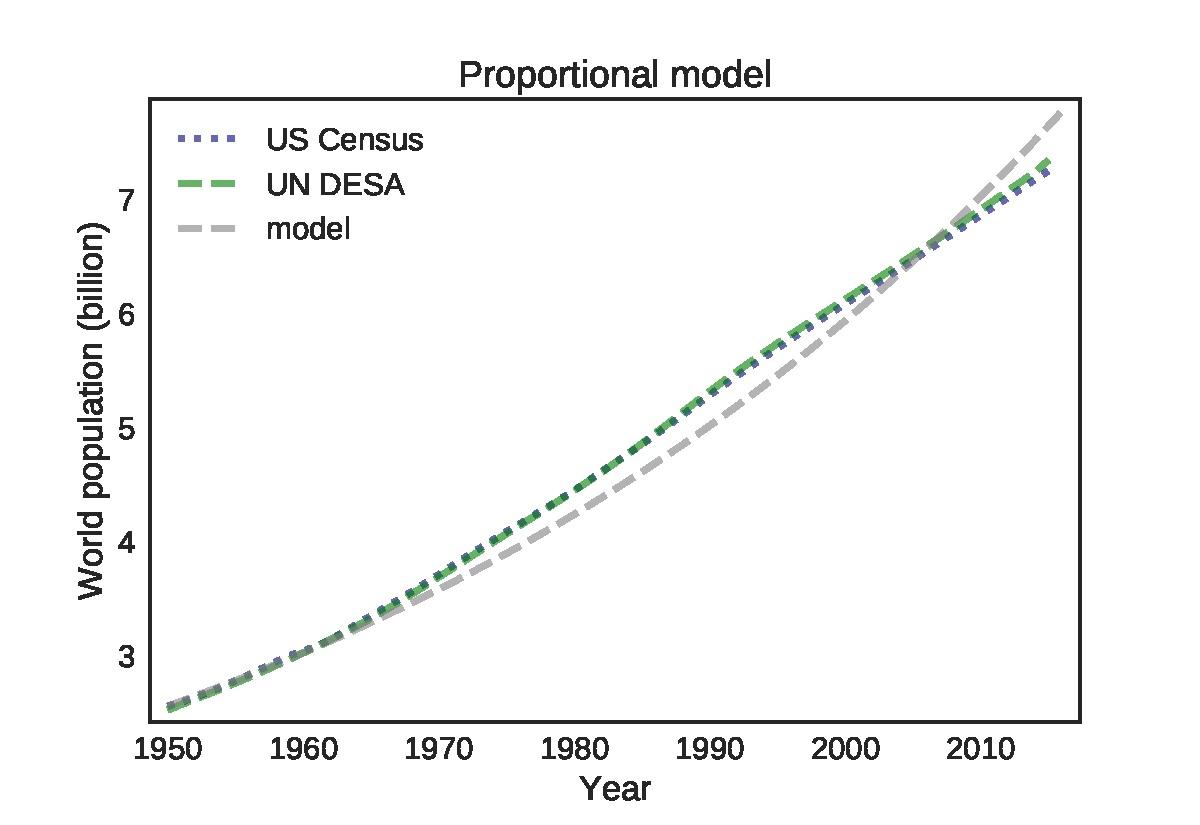
\includegraphics[height=3in]{figs/chap03-fig03.pdf}}
\caption{Estimates of world population, 1950--2015, and a proportional model.}
\label{chap03-fig03}
\end{figure}

Figure~\ref{chap03-fig03} shows the results.  The proportional model fits the data well from 1950 to 1965, but not so well after that.  Overall, the {\bf quality of fit} is not as good as the constant growth model, which is surprising, because it seems like the proportional model is more realistic.

There are a few things we could try to improve the model:

\begin{itemize}

\item Maybe the birth rate and death rate vary over time.

\item Maybe net growth depends on the current population, but the relationship is quadratic, not linear.

\end{itemize}

We will try out these variations, but first, let's clean up the code one more time.

\section{Factoring out the update function}

\py{run_simulation1} and \py{run_simulation2} are nearly identical except for the body of the \py{for} loop, where we compute the population for the next year.
\index{update function}
\index{function!update}

Rather than repeat identical code, we can separate the things that change from the things that don't.  First, we'll pull out the body of the loop and make it a function:

\begin{python}
def update_func1(pop, t, system):
    births = system.birth_rate * pop
    deaths = system.death_rate * pop
    return pop + births - deaths
\end{python}

This function takes as arguments the current population, current year, and a \py{System} object; it returns the computed population for the next year.

Now we can write a function that runs any model:

\begin{python}
def run_simulation(system, update_func):
    results = TimeSeries()
    results[system.t0] = system.p0
    for t in linrange(system.t0, system.t_end):
        results[t+1] = update_func(results[t], t, system)
    system.results = results
\end{python}

This function demonstrates a feature we have not seen before: it takes a function as a parameter!  When we call \py{run_simulation}, the second parameter is a function, like \py{update_func1}, that computes the population for the next year.
\index{function!as parameter}

Here's how we call it:

\begin{python}
run_simulation(system, update_func1)
\end{python}

Passing a function as an argument is the same as passing any other value.  The argument, which is \py{update_func1} in this example, gets assigned to the parameter, which is called \py{update_func}.  Inside \py{run_simulation}, we can run \py{update_func} just like any other function.

When you calls \py{run_simulation}, it calls \py{update_func1} once for each year between \py{t0} and \py{t_end}.  The result is the same as Figure~\ref{chap03-fig03}.


\section{Combining birth and death}

While we are at it, we can also simplify the code by combining births and deaths to compute the net growth rate.  Instead of two parameters, \py{birth_rate} and \py{death_rate}, we can write the update function in terms of a single parameter that represents the difference:

\begin{python}
system.alpha = system.birth_rate - system.death_rate
\end{python}

Here's the modified version of \py{update_func1}:

\begin{python}
def update_func1b(pop, t, system):
    net_growth = system.alpha  * pop
    return pop + net_growth
\end{python}

And here's how we run it:

\begin{python}
run_simulation(system, update_func1b)
\end{python}

Again, the result is the same as Figure~\ref{chap03-fig03}.


\section{Quadratic growth}
\label{quadratic}

It makes sense that net growth should depend on the current population, but maybe it's not a linear relationship, like this:

\begin{python}
    net_growth = system.alpha * pop
\end{python}

Maybe it's a quadratic relationship, like this:
\index{quadratic growth}

\begin{python}
    net_growth = system.alpha * pop + system.beta * pop**2
\end{python}

We can test that conjecture with a new update function:

\begin{python}
def update_func2(pop, t, system):
    net_growth = system.alpha * pop + system.beta * pop**2
    return pop + net_growth
\end{python}

Now we need two parameters.  I chose the following values by trial and error; we will see better ways to do it later.
\index{parameter}

\begin{python}
system.alpha = 0.025
system.beta = -0.0018
\end{python}

And here's how we run it:

\begin{python}
run_simulation(system, update_func2)
\end{python}

\begin{figure}
\centerline{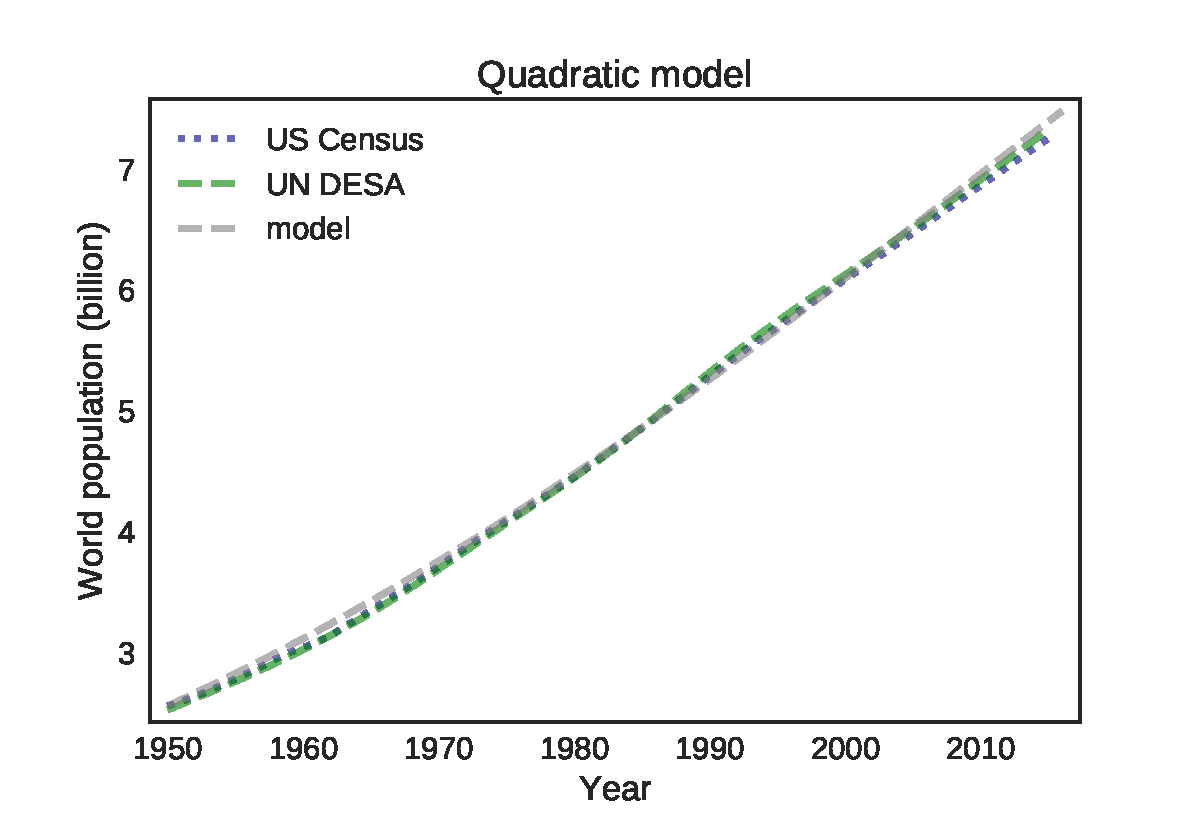
\includegraphics[height=3in]{figs/chap03-fig04.pdf}}
\caption{Estimates of world population, 1950--2015, and a quadratic model.}
\label{chap03-fig04}
\end{figure}

Figure~\ref{chap03-fig04} shows the result.  The model fits the data well over the whole range, with just a bit of daylight between them in the 1960s.

Of course, we should expect the quadratic model to fit better than the linear or proportional model because it has two parameters we can choose, where the other models have only one.  In general, the more parameters you have to play with, the better you should expect the model to fit.
\index{quality of fit}
\index{data}
\index{fitting data}

But fitting the data is not the only reason to think the quadratic model might be a good choice.  It also makes sense; that is, there is a legitimate reason to expect the relationship between growth and population to have this form.

To understand it, let's look at net growth as a function of population.  Here's how we compute it:

\begin{python}
pop_array = linspace(0.001, 15, 100)
net_growth_array = (system.alpha * pop_array + 
                    system.beta * pop_array**2)
\end{python}

\py{pop_array} contains 100 equally spaced values from near 0 to 15.  \py{net_growth_array} contains the corresponding 100 values of net growth.  We can plot the results like this: 

\begin{python}
plot(pop_array, net_growth_array, '-')
\end{python}

\begin{figure}
\centerline{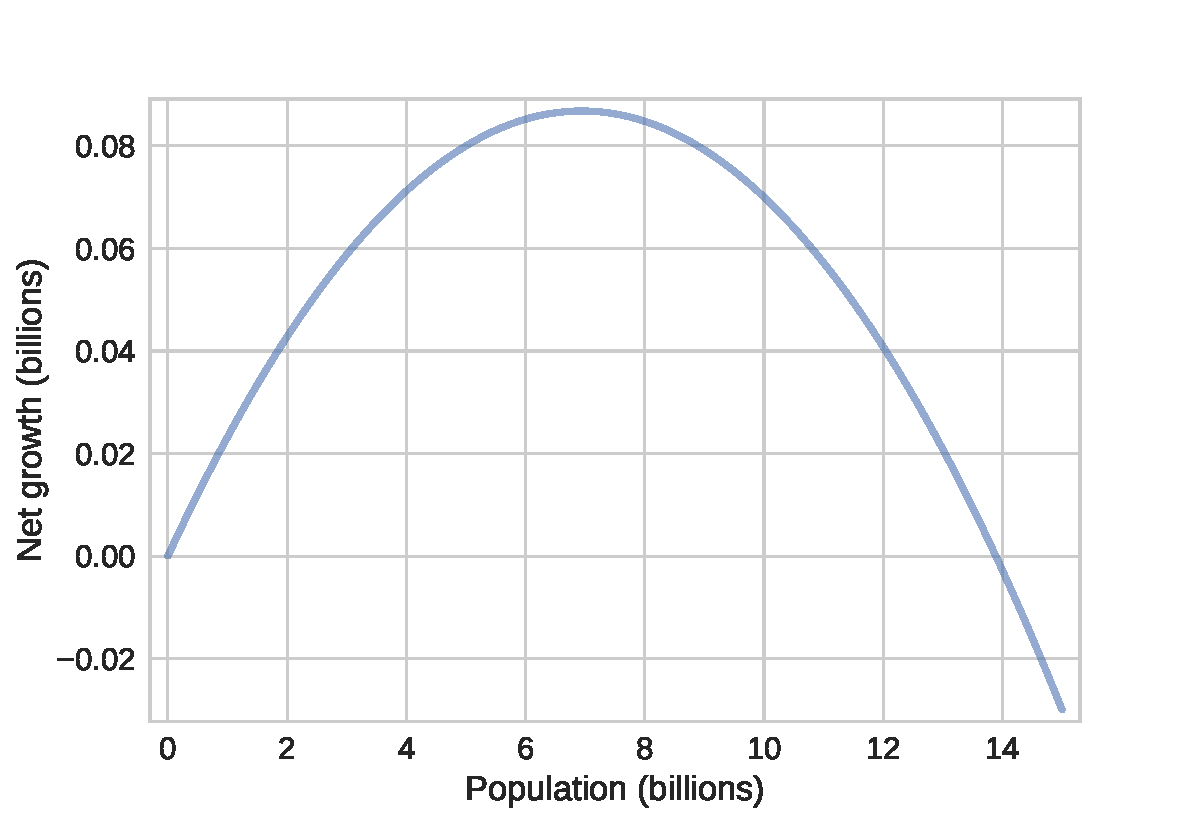
\includegraphics[height=3in]{figs/chap03-fig05.pdf}}
\caption{Net growth as a function of population.}
\label{chap03-fig05}
\end{figure}

Figure~\ref{chap03-fig05} shows the result.  Note that the x-axis is not time, as in the previous figures, but population.  We can divide this curve into four regimes of behavior:
\index{regime}

\begin{itemize}

\item When the population is less than 3-4 billion, net growth is proportional to population, as in the proportional model.  In this regime,  the population grows slowly because the population is small.

\item Between 4 billion and 10 billion, the population grows quickly because there are a lot of people, and there are enough resources, like food, water, and space, to sustain high birth rates and low death rates.

\item Above 10 billion, population grows more slowly because resource limits start to decrease birth rates, increase death rates, or both.

\item Above 14 billion, resources are so limited that the death rate exceeds the birth rate and net growth becomes negative.

\end{itemize}

Just below 14 billion, there is a population where net growth is 0, which means that the population does not change.  At this point, the birth and death rates are equal, so the population is in {\bf equilibrium}.
\index{equilibrium}


\section{Equilibrium}
\label{equilibrium}

To find this equilibrium point, we can find the roots, or zeros, of this equation:
%
\[ \Delta p = \alpha p + \beta p^2 = 0 \]
%
where $\Delta p$ is net growth, $p$ is current population, and $\alpha$ and $\beta$ are the parameters of the model.  We can rewrite the right hand side like this:
%
\[ \Delta p = p (\alpha + \beta p) = 0 \]
%
which is $0$ when $p=0$ or $p=-\alpha/\beta$.  In this example, $\alpha = 0.025$, $\beta = -0.0018$, and $-\alpha/\beta = 13.9$.

In the context of population modeling, the quadratic model is more conventionally written like this:
%
\[ \Delta p = r p (1 - p / K) \]
%
This is the same model; it's just a different way to {\bf parameterize} it.  Given $\alpha$ and $\beta$, we can compute $r=\alpha$ and $K=-\alpha/\beta$.
\index{parameterize}

In this version, it is easier to interpret the parameters: $\alpha$ is the maximum growth rate, observed when $p$ is small, and $K$ is the equilibrium point.  $K$ is also called the {\bf carrying capacity}, since it indicates the maximum population the environment can sustain.
\index{carrying capacity}

In the next chapter we use the models we have developed to generate predictions.


\section{Disfunctions}

When people first learn about functions, there are a few things they often find confusing.  In this section I present and explain some common problems with functions.

As an example, suppose you want a function that takes a \py{System} object, with variables \py{alpha} and \py{beta}, as a parameter and computes the carrying capacity, \py{-alpha/beta}.  Here's a good solution: 

\begin{python}
def carrying_capacity(system):
    K = -system.alpha / system.beta
    return K
    
sys1 = System(alpha=0.025, beta=-0.0018)
pop = carrying_capacity(sys1)
print(pop)
\end{python}

Now let's see all the ways that can go wrong.

Disfunction \#1: Not using parameters.  In the following version, the function doesn't take any parameters; when \py{system} appears inside the function, it refers to the object we created outside the function.

\begin{python}
def carrying_capacity():
    K = -system.alpha / system.beta
    return K
    
system = System(alpha=0.025, beta=-0.0018)
pop = carrying_capacity()
print(pop)
\end{python}

This version actually works, but it is not are versatile as it could be.  If there are several \py{System} objects, this function can only work with one of them, and only if it is named \py{system}.

Disfunction \#2: Clobbering the parameters.  When people first learn about parameters, they often write functions like this:

\begin{python}
# WRONG
def carrying_capacity(system):
    system = System(alpha=0.025, beta=-0.0018)
    K = -system.alpha / system.beta
    return K
    
sys1 = System(alpha=0.03, beta=-0.002)
pop = carrying_capacity(sys1)
print(pop)
\end{python}

In this example, we have a \py{System} object named \py{sys1} that gets passed as an argument to \py{carrying_capacity}.  But when the function runs, it ignores the argument and immediately replaces it with a new \py{System} object.  As a result, this function always returns the same value, no matter what argument is passed.

When you write a function, you generally don't know what the values of the parameters will be.  Your job is to write a function that works for any valid values.  If you assign your own values to the parameters, you defeat the whole purpose of functions.


Disfunction \#3: No return value.  Here's a version that computes the value of \py{K} but doesn't return it.

\begin{python}
# WRONG
def carrying_capacity(system):
    K = -system.alpha / system.beta
    
sys1 = System(alpha=0.025, beta=-0.0018)
pop = carrying_capacity(sys1)
print(pop)
\end{python}

A function that doesn't have a return statement always returns \py{None}, so in this example the value of \py{pop} is \py{None}.  If you are debugging a program and find that the value of a variable is \py{None}, when it shouldn't be, a function without a return statement is a likely cause.


Disfunction \#4: Ignoring the return value.  Finally, here's a version where the function is correct, but the way it's used is not.

\begin{python}
# WRONG
def carrying_capacity(system):
    K = -system.alpha / system.beta
    return K
    
sys1 = System(alpha=0.025, beta=-0.0018)
carrying_capacity(sys1)
print(K)
\end{python}

In this example, \py{carrying_capacity} runs and returns \py{K}, but the return value is dropped.

When you call a function that returns a value, you should do something with the result.  Often you assign it to a variable, as in the previous examples, but you can also use it as part of an expression.  For example, you could eliminate the temporary variable \py{pop} like this:

\begin{python}
print(carrying_capacity(sys1))
\end{python}

Or if you had more than one system, you could compute the total carrying capacity like this:

\begin{python}
total = carrying_capacity(sys1) + carrying_capacity(sys2)
\end{python}

In the notebook for this chapter, you can try out each of these examples and see what happens.


\chapter{Prediction}

In the previous chapter we developed a quadratic model of world population growth from 1950 to 2015.  It is a simple model, but it fits the data well and the mechanisms it's based on are plausible.  

In this chapter we'll use the quadratic model to generate projections of future growth, and compare our results to projections from actual demographers.  Also, we'll represent the models from the previous chapters as differential equations and solve them analytically.
\index{prediction}
\index{projection}

You can view the code for this chapter at \url{http://modsimpy.com/chap04}.  For instructions for downloading and running the code, see Section~\ref{code}.

\section{Generating projections}

We'll start with the quadratic model from Section~\ref{quadratic}, which is based on this update function:
\index{quadratic growth}

\begin{python}
def update_func2(pop, t, system):
    net_growth = system.alpha * pop + system.beta * pop**2
    return pop + net_growth
\end{python}

As we saw in the previous chapter, we can get the start date, end date, and initial population from \py{census}, which is a series that contains world population estimates generated by the U.S. Census:

\begin{python}
t0 = census.index[0]
t_end = census.index[-1]
p0 = census[t0]
\end{python}

Now we can create a \py{System} object:
\index{System object}

\begin{python}
system = System(t0=t0, 
                t_end=t_end,
                p0=p0,
                alpha=0.025,
                beta=-0.0018)
\end{python}

And run the model:

\begin{python}
run_simulation(system, update_func2)
\end{python}

We have already seen the results in Figure~\ref{chap03-fig04}.  Now, to generate a projection, the only thing we have to change is \py{t_end}:

\begin{python}
system.t_end = 2250
run_simulation(system, update_func2)
\end{python}

\begin{figure}
\centerline{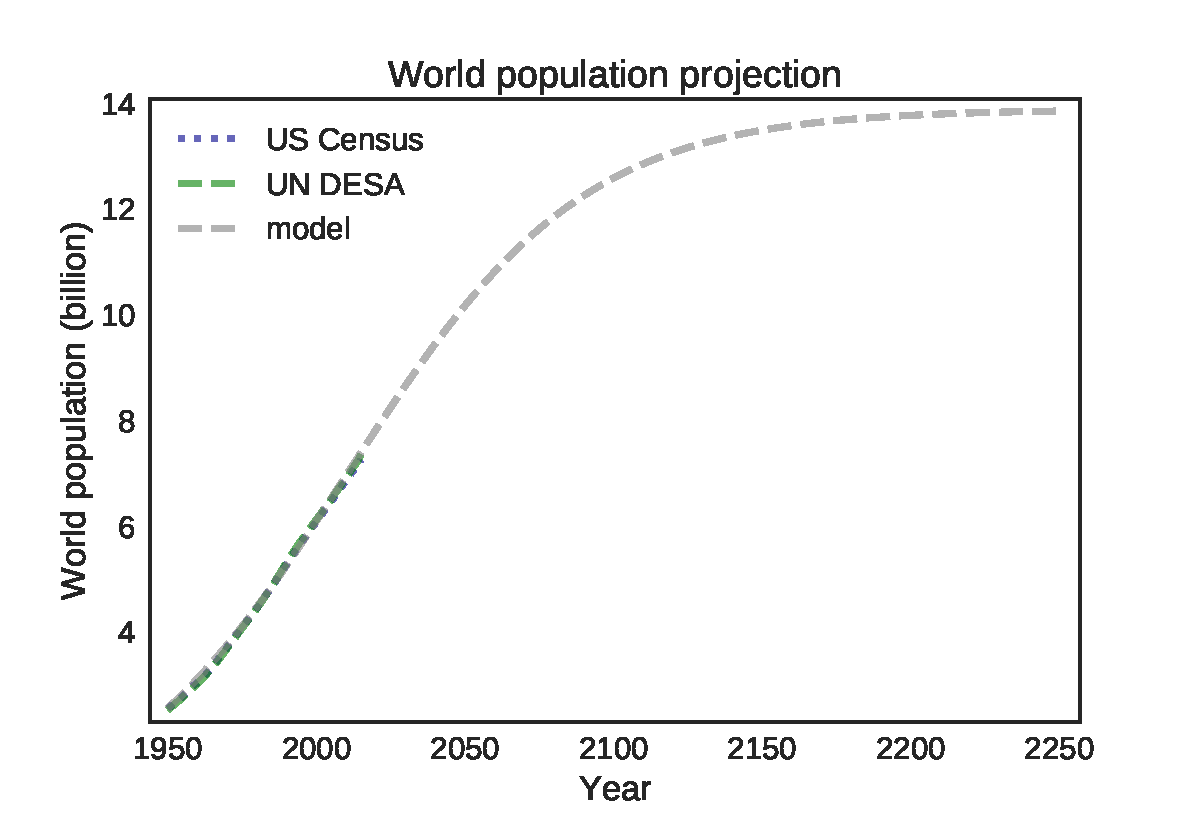
\includegraphics[height=3in]{figs/chap04-fig01.pdf}}
\caption{Quadratic model of world population growth, with projection from 2016 to 2250.}
\label{chap04-fig01}
\end{figure}

Figure~\ref{chap04-fig01} shows the result, with a projection until 2250.  According to this model, population growth will continue almost linearly for the next 50--100 years, then slow over the following 100 years, approaching 13.9 billion by 2250.

I am using the word ``projection" deliberately, rather than ``prediction", with the following distinction: ``prediction" implies something like ``this is what we should reasonably expect to happen, at least approximately"; ``projection" implies something like ``if this model is actually a good description of what is happening in this system, and if nothing in the future causes the parameters of the model to change, this is what would happen."

Using ``projection" leaves open the possibility that there are important things in the real world that are not captured in the model.  It also suggests that, even if the model is good, the parameters we estimate based on the past might be different in the future.

The quadratic model we've been working with is based on the assumption that population growth is limited by the availability of resources; in that scenario, as the population approaches carrying capacity, birth rates fall and death rates rise because resources become scarce.
\index{carrying capacity}

If that assumption is valid, we might be able to use actual population growth to estimate carrying capacity, especially if we observe the transition into the regime where the growth rate starts to fall.

But in the case of world population growth, those conditions don't apply.  Over the last 50 years, the net growth rate has leveled off, but not yet started to fall, so we don't have enough data to make a credible estimate of carrying capacity.  And resource limitations are probably {\em not} the primary reason growth has slowed.  As evidence, consider:

\begin{itemize}

\item First, the death rate is not increasing; rather, it has declined from 1.9\% in 1950 to 0.8\% now (see \url{http://modsimpy.com/mortality}).  So the decrease in net growth is due entirely to declining birth rates.
\index{mortality rate}

\item Second, the relationship between resources and birth rate is the opposite of what the model assumes; as nations develop and people become more wealthy, birth rates tend to fall.  
\index{birth rate}

\end{itemize} 

We should not take too seriously the idea that this model can estimate carrying capacity.  But the predictions of a model can be credible even if the assumptions of the model are not strictly true.  For example, population growth might behave {\em as if} it is resource limited, even if the actual mechanism is something else.

In fact, demographers who study population growth often use models similar to ours.  In the next section, we'll compare our projections to theirs.


\section{Comparing projections}

Table 3 from \url{http://modsimpy.com/worldpop} contains projections from the U.S. Census and the United Nations DESA:

\begin{python}
table3 = tables[3]
\end{python}

For some years, one agency or the other has not published a projection, so some elements of \py{table3} contain the special value \py{NaN}, stands for ``not a number".  \py{NaN} is often used to indicate missing data.
\index{not a number}
\index{NaN}
\index{missing data}

\begin{figure}
\centerline{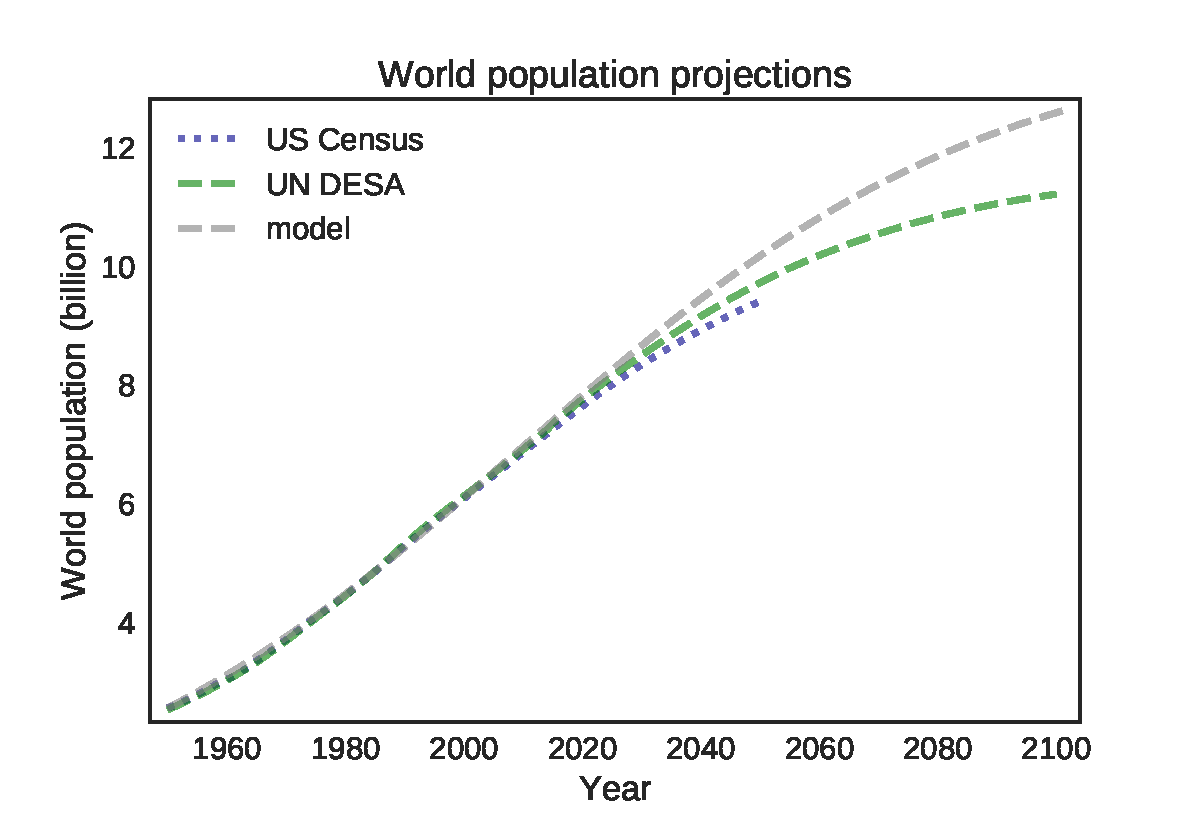
\includegraphics[height=3in]{figs/chap04-fig02.pdf}}
\caption{Projections of world population generated by the U.S. Census Bureau, the United Nations, and our quadratic model.}
\label{chap04-fig02}
\end{figure}

Pandas provides functions that deal with missing data, including \py{dropna}, which removes any elements in a series that contain \py{NaN}.  Using \py{dropna}, we can plot the projections like this:
\index{Pandas}
\index{dropna}

\begin{python}
def plot_projections(table):
    census = table.census / 1e9
    un = table.un / 1e9
    
    plot(census.dropna(), ':', 
         color='darkblue', label='US Census')
    plot(un.dropna(), '--', 
         color='green', label='UN DESA')
\end{python}

We can run our model over the same interval:

\begin{python}
system.t_end = 2100
run_simulation(system, update_func2)
\end{python}

And compare our projections to theirs.  Figure~\ref{chap04-fig02} shows the results.  Real demographers expect world population to grow more slowly than our model projects, probably because their models are broken down by region and country, where conditions are different, and they take into account expected economic development.
\index{demography}

Nevertheless, their projections are qualitatively similar to ours, and theirs differ from each other almost as much as they differ from ours.  So the results from this model, simple as it is, are not entirely crazy.


\section{Recurrence relations}

The population models in the previous chapter and this one are simple enough that we didn't really need to run simulations.  We could have solved them mathematically.  For example, we wrote the constant growth model like this:

\begin{python}
model[t+1] = model[t] + annual_growth
\end{python}

In mathematical notation, we would write the same model like this:
%
\[ x_{n+1} = x_n + c \]
%
where $x_n$ is the population during year $n$, $x_0$ is a given initial population, and $c$ is constant annual growth.  This way of representing the model is a {\bf recurrence relation}; see \url{http://modsimpy.com/recur}.
\index{recurrence relation}

Often it is possible to solve a recurrence relation by writing an equation that computes $x_n$, for a given value of $n$, directly; that is, without computing the intervening values from $x_1$ through $x_{n-1}$.

In the case of constant growth we can see that $x_1 = x_0 + c$, and $x_2 = x_1 + c$.  Combining these, we get $x_2 = x_0 + 2c$, then $x_3 = x_0 + 3c$, and it is not hard to conclude that in general
%
\[ x_n = x_0 + nc \]
%
So if we want to know $x_{100}$ and we don't care about the other values, we can compute it with one multiplication and one addition.

We can also write the proportional model as a recurrence relation:
%
\[ x_{n+1} = x_n + \alpha x_n \]
%
Or more conventionally as:
%
\[ x_{n+1} = x_n (1 + \alpha) \]
%
Now we can see that $x_1 = x_0 (1 + \alpha)$, and $x_2 = x_0 (1 + \alpha)^2$, and in general
%
\[ x_n = x_0 (1 + \alpha)^n \]
%
This result is a {\bf geometric progression}; see \url{http://modsimpy.com/geom}.  When $\alpha$ is positive, the factor $1+\alpha$ is greater than 1, so the elements of the sequence grow without bound.
\index{geometric progression}
\index{quadratic growth}

Finally, we can write the quadratic model like this:
%
\[ x_{n+1} = x_n + \alpha x_n + \beta x_n^2 \]
%
or with the more conventional parameterization like this:
%
\[ x_{n+1} = x_n + r x_n (1 - x_n / K) \]
%
There is no analytic solution to this equation, but we can approximate it with a differential equation and solve that, which is what we'll do in the next section.


\section{Differential equations}
\label{diffeq}

Starting again with the constant growth model
%
\[ x_{n+1} = x_n + c \]
%
If we define $\Delta x$ to be the change in $x$ from one time step to the next, we can write:
%
\[ \Delta x = x_{n+1} - x_n = c \]
%
If we define $\Delta t$ to be the time step, which is one year in the example, we can write the rate of change per unit of time like this:
%
\[ \frac{\Delta x}{\Delta t} = c \]
%
This model is {\bf discrete}, which means it is only defined at integer values of $n$ and not in between.  But in reality, people are born and die all the time, not once a year, so a {\bf continuous} model might be more realistic.
\index{discrete}
\index{continuous}
\index{time step}

We can make this model continuous by writing the rate of change in the form of a derivative:
%
\[ \frac{dx}{dt} = c \]
%
This way of representing the model is a {\bf differential equation}; see \url{http://modsimpy.com/diffeq}.
\index{differential equation}

We can solve this differential equation if we multiply both sides by $dt$:
%
\[ dx = c dt \]
%
And then integrate both sides:
%
\[ x(t) = c t + x_0 \]
%
Similarly, we can write the proportional growth model like this:
%
\[ \frac{\Delta x}{\Delta t} = \alpha x \]
%
And as a differential equation like this:
%
\[ \frac{dx}{dt} = \alpha x \]
%
If we multiply both sides by $dt$ and divide by $x$, we get
%
\[ \frac{1}{x}~dx = \alpha~dt \] 
%
Now we integrate both sides, yielding:
%
\[ \ln x = \alpha t + K \]
%
where $\ln$ is the natural logarithm and $K$ is the constant of integration.  Exponentiating both sides, we have
%
\[ \exp(\log(x)) = x = \exp(\alpha t + K) \]
%
which we can rewrite
%
\[ x = \exp(\alpha t) \exp(K) \]
%
Since $K$ is an arbitrary constant, $\exp(K)$ is also an arbitrary constant, so we can write
%
\[ x = C \exp(\alpha t) \]
%
where $C = \exp(K)$.  There are many solutions to this differential equation, with different values of $C$.  The particular solution we want is the one that has the value $x_0$ when $t=0$.  Well, when $t=0$, $x(t) = C$, so $C = x_0$ and the solution we want is
%
\[ x(t) = x_0 \exp(\alpha t) \]
%
If you would like to see this derivation done more carefully, you might like this video: \url{http://modsimpy.com/khan1}.
\index{logarithm}
\index{exponentiation}
\index{integration}
\index{constant of integration}

\section{Analysis and simulation}

Once you have designed a model, there are generally two ways to proceed: simulation and analysis.  Simulation often comes in the form of a computer program that models changes in a system over time, like births and deaths, or bikes moving from place to place.  Analysis often comes in the form of algebra; that is, symbolic manipulation using mathematical notation.
\index{analysis}
\index{algebra}
\index{symbolic manipulation}

Analysis and simulation have different capabilities and limitations.  Simulation is generally more versatile; it is easy to add and remove parts of a program and test many versions of a model, as we have done in the previous examples.

But there are several things we can do with analysis that are harder or impossible with simulations:

\begin{itemize}

\item With analysis we can sometimes compute, exactly and efficiently, a value that we could only approximate, less efficiently, with simulation.  For example, in Figure~\ref{chap03-fig05}, we can see that net growth goes to zero near 14 billion, and we could estimate carrying capacity using a numerical search algorithm (more about that later).  But with the analysis in Section~\ref{quadratic}, we get the general result that $K=-\alpha/\beta$.

\item Analysis often provides ``computational shortcuts", that is, the ability to jump forward in time to compute the state of a system many time steps in the future without computing the intervening states.
\index{time step}

\item We can use analysis to state and prove generalizations about models; for example, we might prove that certain results will always or never occur.  With simulations, we can show examples and sometimes find counterexamples, but it is hard to write proofs.
\index{proof}

\item Analysis can provide insight into models and the systems they describe; for example, sometimes we can identify regimes of qualitatively different behavior and key parameters that control those behaviors.
\index{regime}

\end{itemize}

When people see what analysis can do, they sometimes get drunk with power, and imagine that it gives them a special ability to see past the veil of the material world and discern the laws of mathematics that govern the universe.  When they analyze a model of a physical system, they talk about ``the math behind it" as if our world is the mere shadow of a world of ideal mathematical entities\footnote{I am not making this up; see \url{http://modsimpy.com/plato}.}.
\index{Plato}

This is, of course, nonsense.  Mathematical notation is a language designed by humans for a purpose, specifically to facilitate symbolic manipulations like algebra.  Similarly, programming languages are designed  for a purpose, specifically to represent computational ideas and run programs.
\index{math notation}
\index{programming languages}

Each of these languages is good for the purposes it was designed for and less good for other purposes.  But they are often complementary, and one of the goals of this book is to show how they can be used together.


\section{Analysis with WolframAlpha}

Until recently, most analysis was done by dragging sticks of graphite across wood pulp\footnote{Or ``rubbing the white rock on the black rock", a line I got from Woodie Flowers, who got it from Stephen Jacobsen.}, a process that is laborious and error-prone.  A useful alternative is symbolic computation.  If you have used services like WolframAlpha, you have used symbolic computation.
\index{symbolic computation}
\index{WolframAlpha}

For example, if you go to \url{https://www.wolframalpha.com/} and type

\begin{python}
df(t) / dt = alpha f(t)
\end{python}

WolframAlpha infers that \py{f(t)} is a function of \py{t} and \py{alpha} is a parameter; it classifies the query as a ``first-order linear ordinary differential equation", and reports the general solution:
%
\[ f(t) = c_1 \exp(\alpha t) \]
%
If you add a second equation to specify the initial condition:

\begin{python}
df(t) / dt = alpha f(t),  f(0) = p0
\end{python}

WolframAlpha reports the particular solution:

\[ f(t) = p_0 \exp(\alpha t) \]

WolframAlpha is based on Mathematica, a powerful programming language designed specifically for symbolic computation.
\index{Mathematica}

\section{Analysis with SymPy}

Python has a library called SymPy that provides symbolic computation tools similar to Mathematica.  They are not as easy to use as WolframAlpha, but they have some other advantages.
\index{SymPy}

Before we can use SymPy, we have to import it:
\index{import statement}
\index{statement!import}

\begin{python}
from sympy import *
\end{python}

SymPy defines many functions, and some of them conflict with functions defined in \py{modsim} and the other libraries we're using, I suggest that you do symbolic computation with SymPy in a separate notebook.

The code for this section and the next is in this notebook: \url{http://modsimpy.com/sympy04}.  

SymPy defines a \py{Symbol} object that represents symbolic variable names, functions, and other mathematical entities.
\index{Symbol} object

SymPy provides a function called \py{symbols} that takes a string and returns a \py{Symbol} object.  So if we run this assignment:

\begin{python}
t = symbols('t')
\end{python}

Python understands that \py{t} is a symbol, not a numerical value.  If we now run

\begin{python}
expr = t + 1
\end{python}

Python doesn't try to perform numerical addition; rather, it creates a new \py{Symbol} that represents the sum of \py{t} and \py{1}.  We can evaluate the sum using \py{subs}, which substitutes a value for a symbol.  This example substitutes 2 for \py{t}:

\begin{python}
expr.subs(t, 2)
\end{python}

The result is 3.  Functions in SymPy are represented by a special kind of \py{Symbol}:

\begin{python}
f = Function('f')
\end{python}

Now if we write \py{f(t)}, we get an object that represents the evaluation of a function, $f$, at a value, $t$.  But again it doesn't actually try to evaluate it.


\section{Differential equations in SymPy}

SymPy provides a function, \py{diff}, that can differentiate a function.  We can apply it to \py{f(t)} like this:
\index{differential equation}
\index{SymPy}

\begin{python}
dfdt = diff(f(t), t)
\end{python}

The result is a \py{Symbol} that represents the derivative of \py{f} with respect to \py{t}.  But again, SymPy doesn't try to compute the derivative yet.
\index{Symbol object}

To represent a differential equation, we use \py{Eq}:

\begin{python}
alpha = symbols('alpha')
eq1 = Eq(dfdt, alpha*f(t))
\end{python}

The result is an object that represents an equation, which is displayed like this:
%
\[ \frac{d}{d t} f{\left (t \right )} = \alpha f{\left (t \right )} \]
%
Now we can use \py{dsolve} to solve this differential equation:

\begin{python}
solution_eq = dsolve(eq1)
\end{python}

The result is the equation
%
\[ f{\left (t \right )} = C_{1} \exp(\alpha t) \]
%
This is the {\bf general solution}, which still contains an unspecified constant, $C_1$.  To get the {\bf particular solution} where $f(0) = p_0$, we substitute \py{p0} for \py{C1}.  First, we have to create two more symbols:
\index{general solution}
\index{particular solution}

\begin{python}
C1, p0 = symbols('C1 p0')
\end{python}

Now we can perform the substitution:

\begin{python}
particular = solution_eq.subs(C1, p0)
\end{python}

The result is 
%
\[ f{\left (t \right )} = p_{0} \exp(\alpha t) \]
%
This function is called the {\bf exponential growth curve}; see \url{http://modsimpy.com/expo}.
\index{exponential growth}

\section{Solving the quadratic growth model}

In the notebook for this chapter, you will see how to use the same tools to solve the quadratic growth model with parameters $r$ and $K$.  The general solution is
%
\[ f{\left (t \right )} = \frac{K \exp(C_{1} K + r t)}{\exp(C_{1} K + r t) - 1} \]
%
To get the particular solution where $f(0) = p_0$, we evaluate the general solution at $t=0$, which yields:
%
\[ f(0) = \frac{K \exp(C_{1} K)}{\exp(C_{1} K) - 1} \]
%
Then we set this expression equal to $p_0$ and solve for $C_1$.  The result is:
%
\[ C_1 = \frac{1}{K} \log{\left (- \frac{p_{0}}{K - p_{0}} \right )} \]
%
Finally, we substitute this value of $C_1$ into the general solution, which yields:
%
\[ f(t) = \frac{K p_{0} \exp(r t)}{K + p_{0} \exp(r t) - p_{0}} \]
%
This function is called the {\bf logistic growth curve}; see \url{http://modsimpy.com/logistic}.  In the context of growth models, the logistic function is often written, equivalently,
%
\[ f(t) = \frac{K}{1 + A \exp(-rt)} \]
%
where $A = (K - p_0) / p_0$.

If you would like to see this differential equation solved by hand, you might like this video: \url{http://modsimpy.com/khan2}
\index{quadratic growth}
\index{logistic function}

\section{Summary}

The following tables summarize the results so far:

\begin{tabular}{l|l} 
\hline
Growth type         & Discrete (difference equation) \\ 
\hline 
Constant & linear: $x_n = p_0 + \alpha n$  \\ 
 
Proportional & geometric: $x_n = p_0(1+\alpha)^n$  \\ 

\end{tabular} 

\begin{tabular}{l|l} 
\hline
        & Continuous (differential equation) \\ 
\hline 
Constant & linear: $x(t) = p_0 + \alpha t$ \\ 
 
Proportional & exponential: $x(t) = p_0 \exp(\alpha t)$ \\ 
 
Quadratic & logistic: $x(t) = K / (1 + A\exp(-rt))$ \\ 
\end{tabular} 

What I've been calling the constant growth model is more commonly called ``linear growth" because the solution is a line.  Similarly, what I've called proportional is commonly called ``exponential", and what I've called quadratic is commonly called ``logistic".
\index{logistic growth}

I avoided the more common terms until now because I thought it would be strange to use them before we solved the equations and discovered the functional form of the solutions.


\chapter{Design}

In the previous chapter, we developed a model of world population growth and used it to generate projections for the next 100 years.  In this chapter, we develop a model of an epidemic as it spreads in a susceptible population, and use it to evaluate the effectiveness of possible interventions.
\index{epidemic}

My presentation of the SIR model in this chapter, and the analysis in the next chapter, is based on an excellent article by David Smith and Lang Moore\footnote{Smith and Moore, ``The SIR Model for Spread of Disease," Journal of Online Mathematics and its Applications, December 2001, at \url{http://modsimpy.com/sir}.}.
\index{SIR model}

You can view the code for this chapter at \url{http://modsimpy.com/chap05}.  For instructions for downloading and running the code, see Section~\ref{code}.


\section{The Freshman Plague}

Every year at Olin College, about 90 new students come to campus from around the country and the world.  Most of them arrive healthy and happy, but usually at least one brings with them some kind of infectious disease.  A few weeks later, predictably, some fraction of the incoming class comes down with what we call ``The Freshman Plague".
\index{Olin College}
\index{Freshman Plague}
\index{Kermack-McKendrick}

In this chapter we introduce a well-known model of infectious disease, the Kermack-McKendrick model, and use it to explain the progression of the disease over the course of the semester, predict the effect of possible interventions (like immunization) and design the most effective intervention campaign.
\index{disease}
\index{infection}
\index{design}

So far we have done our own modeling; that is, we've chosen physical systems, identified factors that seem important, and made decisions about how to represent them.  In this chapter we start with an existing model and reverse-engineer it.  Along the way, we consider the modeling decisions that went into it and identify its capabilities and limitations.

\section{The SIR model}

The Kermack-McKendrick model is a simple version of an {\bf SIR model}, so-named because it considers three categories of people:

\begin{itemize}

\item {\bf S}: People who are ``susceptible", that is, capable of contracting the disease if they come into contact with someone who is infected.

\item {\bf I}: People who are ``infected" or, more specifically, capable of passing along the disease if they come into contact with someone susceptible.

\item {\bf R}: People who are ``recovered" or, for deadly diseases, ``removed".

\end{itemize}
  
In the basic version of the model, people who have recovered are considered to be immune to reinfection.  That is a reasonable model for some diseases, but not for others, so it should be on the list of assumptions to reconsider later.

Let's think about how the number of people in each category changes over time.  Suppose we know that people with the disease are infectious for a period of 4 days, on average.  If 100 people are infectious at a particular point in time, and we ignore the particular time each one became infected, we expect about 1 out of 4 to recover on any particular day.

Putting that a different way, if the time between recoveries is 4 days, the recovery rate is about 0.25 recoveries per day, which we'll denote with the parameter $\gamma$ (the Greek letter gamma).  If the total number of people in the population is $N$, and the fraction currently infected is $i$, the total number of recoveries we expect per day is $\gamma i N$.
\index{recovery rate}

Now let's think about the number of new infections.  Suppose we know that each susceptible person comes into contact with 1 person every 3 days, on average, in such a way that they would contract the disease if the other person is infected.  We'll denote this contact rate with the parameter $\beta$ (the Greek letter beta).
\index{infection rate}

It's probably not reasonable to assume that we know $\beta$ ahead of time, but later we'll see how to estimate it based on data from previous semesters.

If $s$ is the fraction of the population that's susceptible, $s N$ is the number of susceptible people, $\beta s N$ is the number of contacts per day, and $\beta s i N$ is the number of those contacts where the other person is infectious.
\index{susceptible}

In summary:

\begin{itemize}

\item The number of recoveries we expect per day is $\gamma i N$; dividing by $N$ yields the fraction of the population that recovers in a day, which is $\gamma i$.

\item The number of new infections we expect per day is $\beta s i N$; dividing by $N$ yields the fraction of the population that gets infected in a day, which is $\beta s i$.

\end{itemize}

This model assumes that the population is closed, that is, no one arrives or departs.  So the size of the population, $N$, is constant.


\section{The SIR equations}
\label{sireqn}

If we treat time as a continuous quantity, we can write differential equations that describe the rates of change for $s$, $i$, and $r$ (where $r$ is the fraction of the population that has recovered):
%
\begin{align*}
\frac{ds}{dt} &= -\beta s i \\
\frac{di}{dt} &= \beta s i - \gamma i\\
\frac{dr}{dt} &= \gamma i
\end{align*}
%
To avoid cluttering the equations, I leave it implied that $s$ is a function of time, $s(t)$, and likewise for $i$ and $r$.
\index{differential equation}

SIR models are examples of {\bf compartment models}, so-called because they divide the world into discrete categories, or compartments, and describe transitions from one compartment to another.  Compartments are also called {\bf stocks} and transitions between them are called {\bf flows}.
\index{compartment model}
\index{stock}
\index{flow}
\index{stock and flow diagram}

In this example, there are three stocks --- susceptible, infected, and recovered --- and two flows --- new infections and recoveries.  Compartment models are often represented visually using stock-and-flow diagrams (see \url{http://modsimpy.com/stock}.
Figure~\ref{stock_flow1} shows the stock and flow diagram for an SIR model.

\begin{figure}
%http://yuml.me/edit/3de9c163
\centerline{\includegraphics[width=4.5in]{figs/stock_flow1.pdf}}
\caption{Stock and flow diagram for an SIR model.}
\label{stock_flow1}
\end{figure}




\section{Implementation}

For a given physical system, there are many possible models, and for a given model, there are many ways to represent it.  For example, we can represent an SIR model as a stock-and-flow diagram, as a set of differential equations, or as a Python program.  The process of representing a model in these forms is called {\bf implementation}.  In this section, we implement the SIR model in Python.
\index{implementation}

As a first step, I'll represent the initial state of the system using a \py{State} object, which is defined in the \py{modsim} library.  A \py{State} object is a collection of {\bf state variables}; each state variable represents information about the system that changes over time.  In this example, the state variables are \py{S}, \py{I}, and \py{R}; they represent the fraction of the population in each compartment.
\index{System object}
\index{State object}
\index{state variable}

Creating a \py{State} object is similar to creating a \py{System} object.  We can initialize the \py{State} object with the {\em number} of people in each compartment:

\begin{python}
init = State(S=89, I=1, R=0)
\end{python}

And then convert the numbers to fractions by dividing by the total:

\begin{python}
init /= sum(init)
\end{python}

For now, let's assume we know the time between contacts and time between recoveries:

\begin{python}
tc = 3             # time between contacts in days 
tr = 4             # recovery time in days
\end{python}

In that case we can compute the parameters of the model:

\begin{python}
beta = 1 / tc      # contact rate in per day
gamma = 1 / tr     # recovery rate in per day
\end{python}

Now we need a \py{System} object to store the parameters and initial conditions.  The following function takes the system parameters as function parameters and returns a new \py{System} object:
\index{\py{make_system}}

\begin{python}
def make_system(beta, gamma):
    init = State(S=89, I=1, R=0)
    init /= sum(init)

    t0 = 0
    t_end = 7 * 14

    return System(init=init, t0=t0, t_end=t_end,
                  beta=beta, gamma=gamma)
\end{python}

The default value for \py{t_end} is 14 weeks, about the length of a semester.


\section{The update function}

At any point in time, the state of the system is represented by a \py{State} object with three variables, \py{S}, \py{I} and \py{R}.  Next we'll define an update function that takes the \py{State} object as a parameter, along with the \py{System} object that contains the parameters, and computes the state of the system during the next time step:
\index{update function}
\index{function!update}
\index{time step}

\begin{python}
def update1(state, system):
    s, i, r = state

    infected = system.beta * i * s    
    recovered = system.gamma * i
    
    s -= infected
    i += infected - recovered
    r += recovered
    
    return State(S=s, I=i, R=r)
\end{python}

The first line uses a feature we have not seen before, {\bf multiple assignment}.  The value on the right side is a \py{State} object that contains three values.  The left side is a sequence of three variable names.  The assignment does just what we want: it assigns the three values from the \py{State} object to the three variables, in order.
\index{State object}

The update function computes \py{infected} and \py{recovered} as a fraction of the population, then updates \py{s}, \py{i} and \py{r}.  The return value is a \py{State} that contains the updated values.
\index{return value}

When we call \py{update1} like this:

\begin{python}
state = update1(init, sir)
\end{python}

The result is a \py{State} object with these values:

\begin{tabular}{lr}
 & {\bf \sf value} \\ 
\hline 
{\bf \sf S} & 0.985388 \\ 
{\bf \sf I} & 0.011865 \\ 
{\bf \sf R} & 0.002747 \\ 
\end{tabular} 

%TODO: figure out when to talk about integers and floats (or never)


\section{Running the simulation}

Now we can simulate the model over a sequence of time steps:
\index{time step}

\begin{python}
def run_simulation(system, update_func):
    state = system.init
    for t in linrange(system.t0, system.t_end):
        state = update_func(state, system)
    return state
\end{python}

The parameters of \py{run_simulation} are the \py{System} object and the update function.  The \py{System} object contains the parameters, initial conditions, and values of \py{t0} and \py{t_end}.
\index{\py{run_simulation}}

The outline of this function should look familiar; it is similar to the function we used for the population model in Section~\ref{nowwithsystem}.

We can call \py{run_simulation} like this:

\begin{python}
system = make_system(beta, gamma)
run_simulation(system, update1)
\end{python}

The result is the final state of the system:

\begin{tabular}{lr}
 & {\bf \sf value} \\ 
\hline 
{\bf \sf S} & 0.520819 \\ 
{\bf \sf I} & 0.000676 \\ 
{\bf \sf R} & 0.478505 \\ 
\end{tabular} 

This result indicates that after 14 weeks (98 days), about 52\% of the population is still susceptible, which means they were never infected, less than 1\% are actively infected, and 48\% have recovered, which means they were infected at some point.


\section{Collecting the results}

The previous version of \py{run_simulation} only returns the final state, but we might want to see how the state changes over time.  We'll consider two ways to do that: first, using three \py{TimeSeries} objects, then using a new object called a \py{TimeFrame}.
\index{TimeFrame object}
\index{TimeSeries object}

Here's the first version:

\begin{python}
def run_simulation(system, update_func):
    S = TimeSeries()
    I = TimeSeries()
    R = TimeSeries()

    state = system.init
    t0 = system.t0
    S[t0], I[t0], R[t0] = state
    
    for t in linrange(system.t0, system.t_end):
        state = update_func(state, system)
        S[i+1], I[i+1], R[i+1] = state
    
    system.S = S
    system.I = I
    system.R = R
\end{python}

First, we create \py{TimeSeries} objects to store the results.  Notice that the variables \py{S}, \py{I}, and \py{R} are \py{TimeSeries} objects now.

Next we initialize \py{state}, \py{t0}, and the first elements of \py{S}, \py{I} and \py{R}.  

Inside the loop, we use \py{update_func} to compute the state of the system at the next time step, then use multiple assignment to unpack the elements of \py{state}, assigning each to the corresponding \py{TimeSeries}.
\index{time step}

At the end of the function, we store \py{S}, \py{I}, and \py{R} as system variables.

Now we can run the function like this:

\begin{python}
system = make_system(beta, gamma)
run_simulation(system, update1)
\end{python}

We'll use the following function to plot the results:

\begin{python}
def plot_results(S, I, R):
    plot(S, '--', color='blue', label='Susceptible')
    plot(I, '-', color='red', label='Infected')
    plot(R, ':', color='green', label='Resistant')
    decorate(xlabel='Time (days)',
             ylabel='Fraction of population')
\end{python}

And run it like this:
\index{plot}
\index{decorate}

\begin{python}
plot_results(system.S, system.I, system.R)
\end{python}

\begin{figure}
\centerline{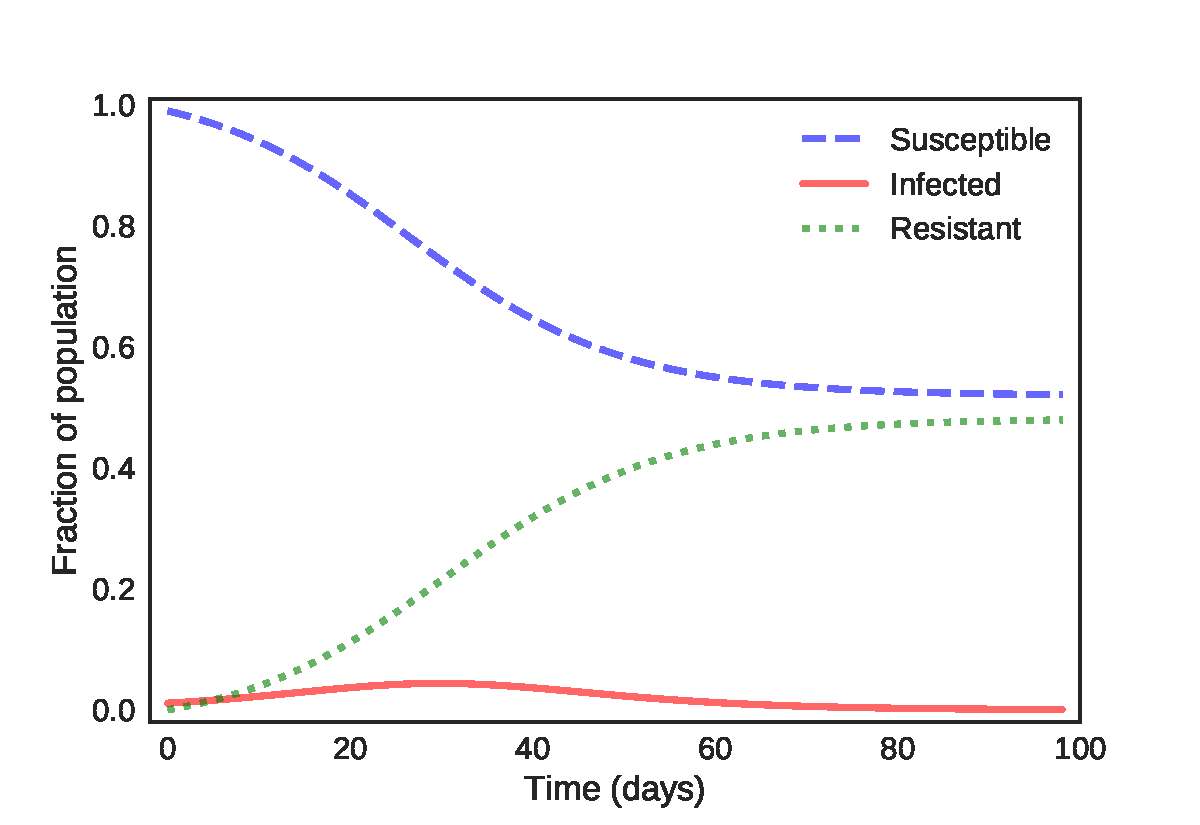
\includegraphics[height=3in]{figs/chap05-fig01.pdf}}
\caption{Time series for \py{S}, \py{I}, and \py{R} over the course of 98 days.}
\label{chap05-fig01}
\end{figure}

Figure~\ref{chap05-fig01} shows the result.  Notice that it takes about three weeks (21 days) for the outbreak to get going, and about six weeks (42 days) before it peaks.  The fraction of the population that's infected is never very high, but it adds up.  In total, almost half the population gets sick. 


\section{Now with a TimeFrame}
\label{timeframe}

If the number of state variables is small, storing them as separate \py{TimeSeries} objects might not be so bad.  But a better alternative is to use a \py{TimeFrame}, which is another object are defined in the \py{modsim} library.
\index{TimeFrame object}
\index{DataFrame object}

A \py{TimeFrame} is almost identical to a \py{DataFrame}, which we used in Section~\ref{worldpopdata}, with just a few changes I made to adapt it for our purposes.  For more details, you can read the \py{modsim} library source code.

Here's a more concise version of \py{run_simulation} using a \py{TimeFrame}:

\begin{python}
def run_simulation(system, update_func):
    frame = TimeFrame(columns=system.init.index)
    frame.loc[system.t0] = system.init
    
    for t in linrange(system.t0, system.t_end):
        frame.loc[i+1] = update_func(frame.loc[i], system)
    
    system.results = frame
\end{python}

The first line creates an empty \py{TimeFrame} with one column for each state variable.  Then, before the loop starts, we store the initial conditions in the \py{TimeFrame} at \py{t0}.  Based on the way we've been using \py{TimeSeries} objects, it is tempting to write:

\begin{python}
frame[system.t0] = system.init
\end{python}

But when you use the bracket operator with a \py{TimeFrame} or \py{DataFrame}, it selects a column, not a row.  For example, to select a column, we could write:
\index{bracket operator}
\index{operator~bracket}

\begin{python}
frame['S']
\end{python}

To select a row, we have to use \py{loc}, which stands for ``location". \py{frame.loc[0]} reads a row from a \py{TimeFrame} and 
\index{loc}

\begin{python}
frame.loc[system.t0] = system.init
\end{python}

assigns the values from \py{system.init} to the first row of \py{df}.  Since the value on the right side is a \py{State}, the assignment matches up the index of the \py{State} with the columns of the \py{TimeFrame}; it assigns the \py{S} value from \py{system.init} to the \py{S} column of the \py{TimeFrame}, and likewise with \py{I} and \py{R}.
\index{assignment}

We can use the same feature to write the loop more concisely, assigning the \py{State} we get from \py{update_func} directly to the next row of \py{df}.  
\index{system variable}

Finally, we store \py{frame} as a new system variable.  We can call this version of \py{run_simulation} like this:

\begin{python}
run_simulation(system, update1)
\end{python}

And plot the results like this:

\begin{python}
frame = system.results
plot_results(frame.S, frame.I, frame.R)
\end{python}

As with a \py{DataFrame}, we can use the dot operator to select columns from a \py{TimeFrame}.
\index{dot operator}
\index{operator!dot}

\section{Metrics}
\label{metrics}

When we plot a time series, we get a view of everything that happened when the model ran, but often we want to boil it down to a few numbers that summarize the outcome.  These summary statistics are called {\bf metrics}.
\index{metric}

% TODO: already defined metrics

In the SIR model, we might want to know the time until the peak of the outbreak, the number of people who are sick at the peak, the number of students who will still be sick at the end of the semester, or the total number of students get sick at any point.

As an example I will focus on the last one --- the total number of sick students --- and we will consider interventions intended to minimize it.

When a person gets infected, they move from \py{S} to \py{I}, so we can compute the total number of infections like this:

\begin{python}
def calc_total_infected(system):
    frame = system.results
    return frame.S[system.t0] - frame.S[system.t_end]
\end{python}

In the notebook that accompanies this chapter, you will have a chance to write functions that compute other metrics.  Two functions you might find useful are \py{max} and \py{idxmax}.
\index{max}
\index{idxmax}
 
If you have a \py{Series} called \py{s}, you can compute the largest value of the series like this:

\begin{python}
largest_value = s.max()
\end{python}

And the label of the largest value like this:

\begin{python}
time_of_largest_value = s.idxmax()
\end{python}

If the \py{Series} is a \py{TimeSeries}, the label you get from \py{idxmax} is a time or date.  You can read more about these functions in the \py{Series} documentation at \url{http://modsimpy.com/series}.
\index{Series}

\section{Immunization}

Models like this are useful for testing ``what if?" scenarios.  As an example, we'll consider the effect of immunization.
\index{immunization}
\index{vaccine}
\index{Freshman Plague}

Suppose there is a vaccine that causes a patient to become immune to the Freshman Plague without being infected.  How might you modify the model to capture this effect?

One option is to treat immunization as a short cut from \py{S} to \py{R}, that is, from susceptible to resistant\footnote{We can be flexible about what \py{R} stands for.}.  We can implement this feature like this:

\begin{python}
def add_immunization(system, fraction):
    system.init.S -= fraction
    system.init.R += fraction
\end{python}

\py{add_immunization} moves the given fraction of the population from \py{S} to \py{R}.  If we assume that 10\% of students are vaccinated at the beginning of the semester, and the vaccine is 100\% effective, we can simulate the effect like this:

\begin{python}
system2 = make_system(beta, gamma)
add_immunization(system2, 0.1)
run_simulation(system2, update1)
\end{python}

For comparison, we can run the same model without immunization and plot the results.  Figure~\ref{chap05-fig02} shows the results, plotting \py{S} as a function of time, with and without immunization.  

\begin{figure}
\centerline{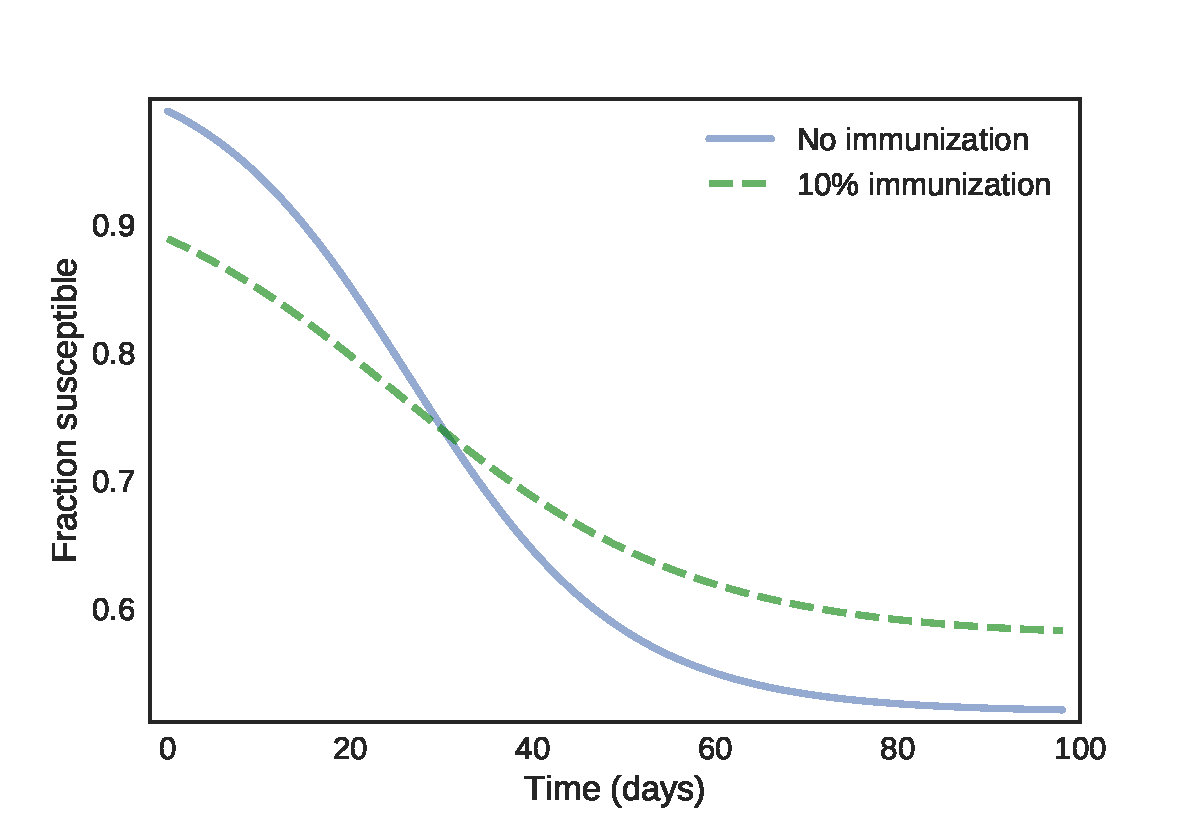
\includegraphics[height=3in]{figs/chap05-fig02.pdf}}
\caption{Time series for \py{S}, with and without immunization.}
\label{chap05-fig02}
\end{figure}

Without immunization, almost 47\% of the population gets infected at some point.  With 10\% immunization, only 31\% gets infected.  That's pretty good.

So let's see what happens if we administer more vaccines.  This following function sweeps a range of immunization rates:
\index{sweep}

\begin{python}
def sweep_immunity(immunize_array):
    sweep = SweepSeries()
    for fraction in immunize_array:
        sir = make_system(beta, gamma)
        add_immunization(sir, fraction)
        run_simulation(sir, update1)
        sweep[fraction] = calc_total_infected(sir)
    return sweep
\end{python}

The parameter of \py{sweep_immunity} is an array of immunization rates.  The result is a \py{SweepSeries} object, which is defined in the \py{modsim} library.  \py{SweepSeries} is similar to \py{TimeSeries}; the difference is that the index of a \py{SweepSeries} contains parameter values, not times.  
\index{SweepSeries object}
\index{parameter sweep}

Figure~\ref{chap05-fig03} shows a plot of the \py{SweepSeries}.  Notice that the x-axis is the immunization rate, not time.

As the immunization rate increases, the number of infections drops steeply.  If 40\% of the students are immunized, fewer than 4\% get sick.  That's because immunization has two effects: it protects the people who get immunized, of course, but it also protects the rest of the population. 

\begin{figure}
\centerline{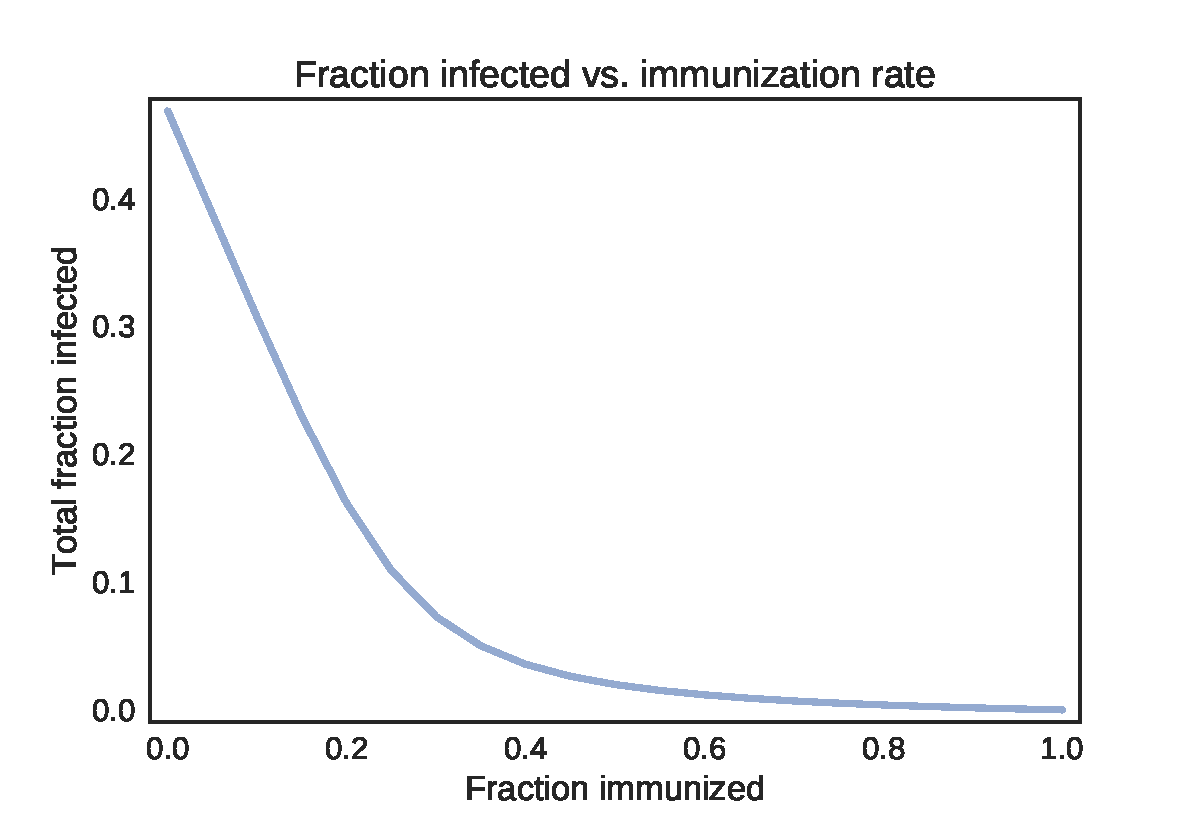
\includegraphics[height=3in]{figs/chap05-fig03.pdf}}
\caption{Fraction of the population infected as a function of immunization rate.}
\label{chap05-fig03}
\end{figure} 

Reducing the number of ``susceptibles" and increasing the number of ``resistants" makes it harder for the disease to spread, because some fraction of contacts are wasted on people who cannot be infected.  This phenomenon is called {\bf herd immunity}, and it is an important element of public health (see \url{http://modsimpy.com/herd}).
\index{herd immunity}

The steepness of the curve in Figure~\ref{chap05-fig03} is a blessing and a curse.  It's a blessing because it means we don't have to immunize everyone, and vaccines can protect the ``herd" even if they are not 100\% effective.

But it's a curse because a small decrease in immunization can cause a big increase in infections.  In this example, if we drop from 80\% immunization to 60\%, that might not be too bad.  But if we drop from 40\% to 20\%, that would trigger a major outbreak, affecting more than 15\% of the population.  For a serious disease like measles, just to name one, that would be a public health catastrophe.
\index{measles}

One use of models like this is to demonstrate phenomena like herd immunity and to predict the effect of interventions like vaccination.  Another use is to evaluate alternatives and guide decision making.  We'll see an example in the next section.


\section{Hand washing}

Suppose you are the Dean of Student Affairs, and you have a budget of just \$1200 to combat the Freshman Plague.  You have two options for spending this money:

\begin{enumerate}

\item You can pay for vaccinations, at a rate of \$100 per dose.

\item You can spend money on a campaign to remind students to wash hands frequently.

\end{enumerate}

We have already seen how we can model the effect of vaccination.  Now let's think about the hand-washing campaign.  We'll have to answer two questions:

\begin{enumerate}

\item How should we incorporate the effect of hand washing in the model?

\item How should we quantify the effect of the money we spend on a hand-washing campaign?

\end{enumerate}

For the sake of simplicity, let's assume that we have data from a similar campaign at another school, showing that a well-funded campaign can change student behavior enough to reduce the infection rate by 20\%.  

In terms of the model, hand washing has the effect of reducing \py{beta}.  That's not the only way we could incorporate the effect, but it seems reasonable and it's easy to implement.

Now we have to model the relationship between the money we spend and the effectiveness of the campaign.  Again, let's suppose we have data from another school that suggests:

\begin{itemize}

\item If we spend \$500 on posters, materials, and staff time, we can change student behavior in a way that decreases the effective value of \py{beta} by 10\%.

\item If we spend \$1000, the total decrease in \py{beta} is almost 20\%.

\item Above \$1000, additional spending has little additional benefit.

\end{itemize}

In the notebook for this chapter you will see how I used a logistic curve to fit this data.  The result is the following function, which takes spending as a parameter and returns \py{factor}, which is the factor by which \py{beta} is reduced:
\index{logistic curve}

\begin{python}
def compute_factor(spending):
    return logistic(spending, M=500, K=0.2, B=0.01)
\end{python}

We use \py{compute_factor} to write \py{add_hand_washing}, which takes a \py{System} object and a budget, and modifies \py{system.beta} to model the effect of hand washing:

\begin{python}
def add_hand_washing(system, spending):
    factor = compute_factor(spending)
    system.beta *= (1 - factor)
\end{python}

Now we can sweep a range of values for \py{spending} and use the simulation to compute the effect:

\begin{python}
def sweep_hand_washing(spending_array):
    sweep = SweepSeries()
    for spending in spending_array:
        sir = make_system(beta, gamma)
        add_hand_washing(sir, spending)
        run_simulation(sir, update1)
        sweep[spending] = calc_total_infected(sir)
    return sweep
\end{python}

Here's how we run it:

\begin{python}
spending_array = linspace(0, 1200, 20)
infected_sweep = sweep_hand_washing(spending_array)
\end{python}

\begin{figure}
\centerline{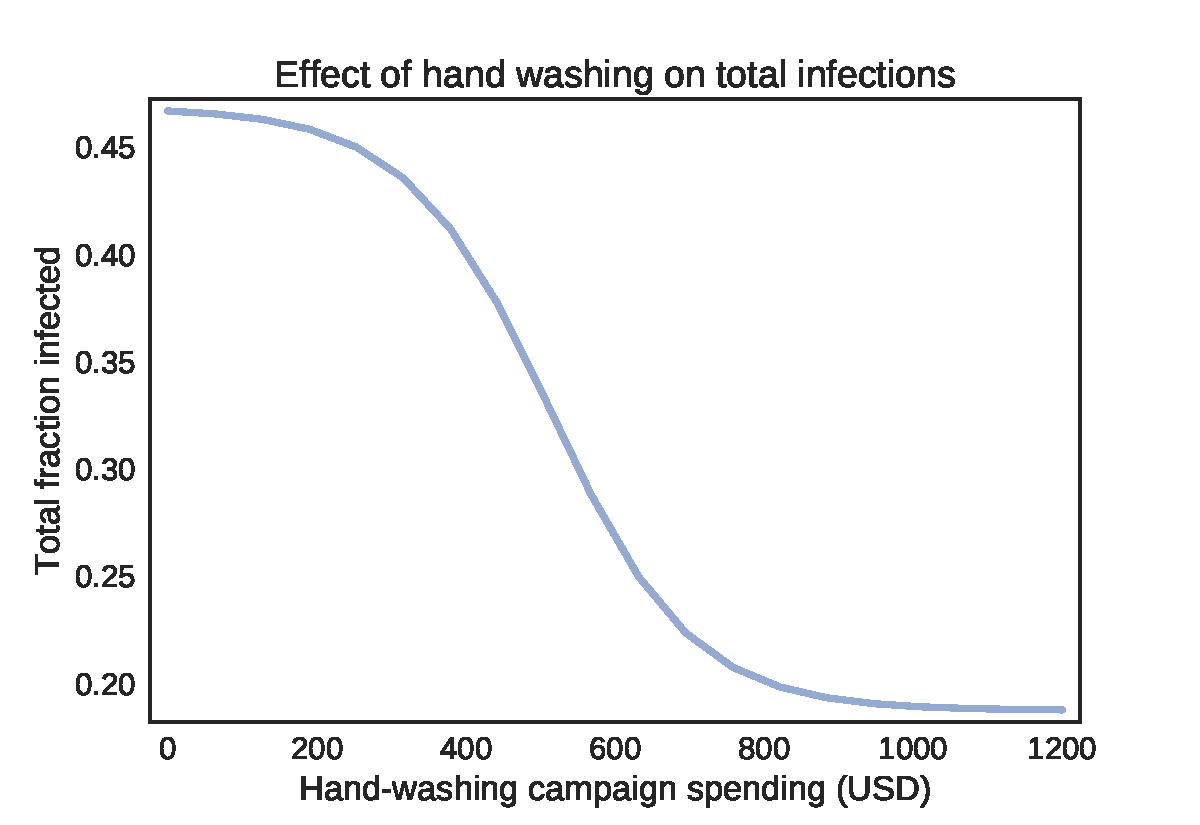
\includegraphics[height=3in]{figs/chap05-fig05.pdf}}
\caption{Fraction of the population infected as a function of hand-washing campaign spending.}
\label{chap05-fig05}
\end{figure} 

Figure~\ref{chap05-fig05} shows the result.  Below \$200, the campaign has little effect.  At \$800 it has a substantial effect, reducing total infections from 46\% to 20\%.  Above \$800, the additional benefit is small.

\section{Optimization} 

Now we can put it all together.  With a fixed budget of \$1200, we have to decide how many doses of vaccine to buy and how much to spend on the hand-washing campaign.
\index{optimization}

Here are the parameters:

\begin{python}
num_students = 90
budget = 1200
price_per_dose = 100
max_doses = int(budget / price_per_dose)
\end{python}

We'll sweep the range of possible doses:

\begin{python}
dose_array = linrange(max_doses)
\end{python}

And run the simulation for each element of \py{dose_array}:

\begin{python}
def sweep_doses(dose_array):
    sweep = SweepSeries()
    for doses in dose_array:
        fraction = doses / num_students
        spending = budget - doses * price_per_dose
        
        sir = make_system(beta, gamma)
        add_immunization(sir, fraction)
        add_hand_washing(sir, spending)
        
        run_simulation(sir, update1)
        sweep[doses] = calc_total_infected(sir)

    return sweep
\end{python}

For each number of doses, we compute the fraction of students we can immunize, \py{fraction} and the remaining budget we can spend on the campaign, \py{spending}.  Then we run the simulation with those quantities and store the number of infections.

\begin{figure}
\centerline{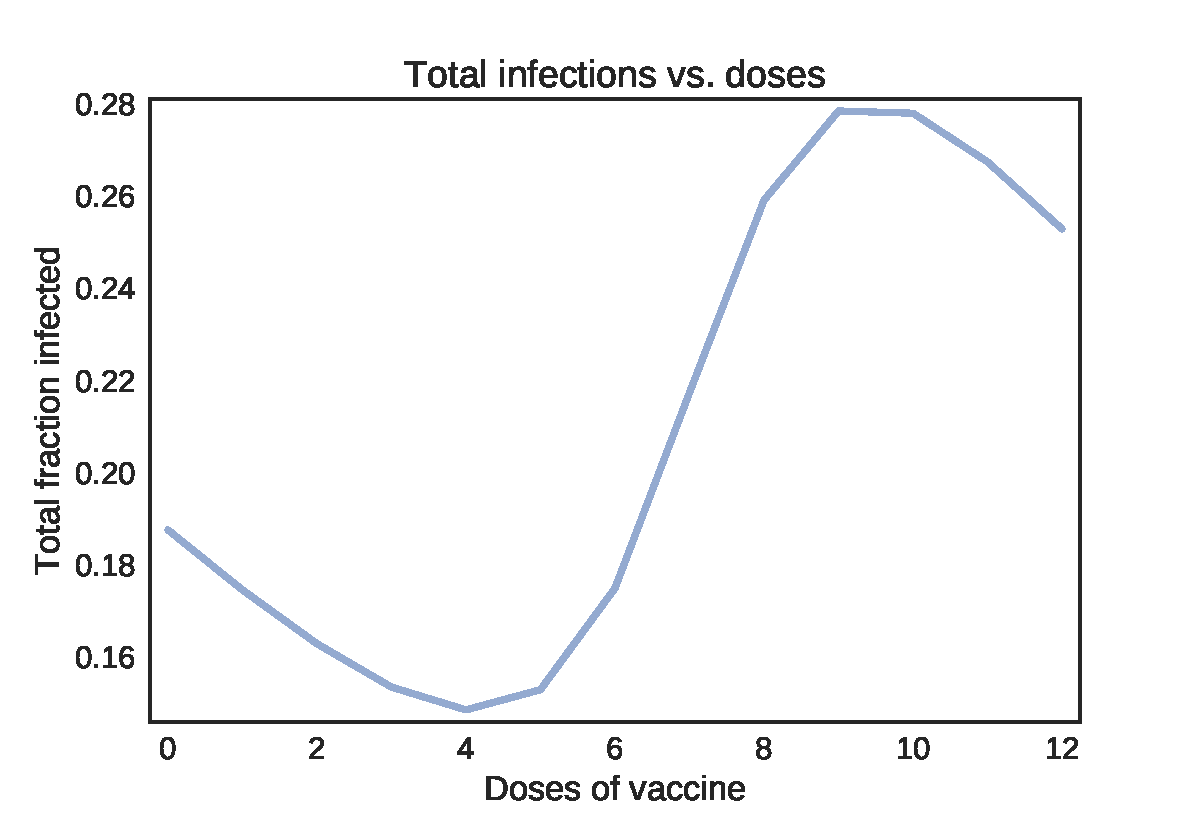
\includegraphics[height=3in]{figs/chap05-fig06.pdf}}
\caption{Fraction of the population infected as a function of the number of doses.}
\label{chap05-fig06}
\end{figure} 

Figure~\ref{chap05-fig06} shows the result.  If we buy no doses of vaccine and spend the entire budget on the campaign, the fraction infected is around 19\%.  At 4 doses, we have \$800 left for the campaign, and this is the optimal point that minimizes the number of students who get sick.

As we increase the number of doses, we have to cut campaign spending, which turns out to make things worse.  But interestingly, when we get above 10 doses, the effect of herd immunity starts to kick in, and the number of sick students goes down again.
\index{herd immunity}

In the notebook for this chapter, you'll have a chance to run this optimization for a few other scenarios.



\chapter{Analysis}

In the previous chapter I presented an SIR model of infectious disease, specifically the Kermack-McKendrick model.  We extended the model to include vaccination and the effect of a hand-washing campaign, and used the extended model to allocate a limited budget optimally, that is, to minimize the number of infections.
\index{Kermack-McKendrick model}
\index{SIR model}

But we assumed that the parameters of the model, contact rate and recovery rate, were known.  In this chapter, we explore the behavior of the model as we vary these parameters, use analysis to understand these relationships better, and propose a method for using data to estimate parameters.

You can view the code for this chapter at \url{http://modsimpy.com/chap06}.  For instructions for downloading and running the code, see Section~\ref{code}.


\section{Unpack}
\label{unpack}

Before we analyze the SIR model, I want to make a few improvements to the code.  In the previous chapter, we used this version of \py{run_simulation}:
\index{\py{run_simulation}}

\begin{python}
def run_simulation(system, update_func):
    frame = DataFrame(columns=system.init.index)
    frame.loc[system.t0] = system.init
    
    for i in linrange(system.t0, system.t_end):
        frame.loc[i+1] = update_func(frame.loc[i], system)
    
    system.results = frame
\end{python}

Because we read so many variables from \py{system}, this code is a bit cluttered.  We can clean it up using \py{unpack}, which is defined in the \py{modsim} library.  \py{unpack} takes a \py{System} object as a parameter and makes the system variables available without using the dot operator.  So we can rewrite \py{run_simulation} like this:
\index{unpack}
\index{System object}

\begin{python}
def run_simulation(system, update_func):
    unpack(system)
    
    frame = TimeFrame(columns=init.index)
    frame.loc[t0] = init
    
    for i in linrange(t0, t_end):
        frame.loc[i+1] = update_func(frame.loc[i], system)
    
    system.results = frame
\end{python}

The variables you unpack should be treated as read-only.  Modifying them is not an error, but it might not have the behavior you expect.  In the notebook for this chapter, you can use \py{unpack} to clean up \py{update1}.


\section{Sweeping beta}

Recall that $\beta$ is the contact rate, which captures both the frequency of interaction between people and the fraction of those interactions that result in a new infection.  If $N$ is the size of the population and $s$ is the fraction that's susceptible, $s N$ is the number of susceptibles, $\beta s N$ is the number of contacts per day between susceptibles and other people, and $\beta s i N$ is the number of those contacts where the other person is infectious.
\index{parameter sweep}

As $\beta$ increases, we expect the total number of infections to increase.  To quantify that relationship, I'll create a range of values for $\beta$:

\begin{python}
beta_array = linspace(0.1, 0.9, 11)
\end{python}

Then run the simulation for each value and print the results.

\begin{python}
for beta in beta_array:
    sir = make_system(beta, gamma)
    run_simulation(sir, update1)
    print(sir.beta, calc_total_infected(sir))
\end{python}

We can wrap that code in a function and store the results in a \py{SweepSeries} object:
\index{SweepSeries object}

\begin{python}
def sweep_beta(beta_array, gamma):
    sweep = SweepSeries()
    for beta in beta_array:
        system = make_system(beta, gamma)
        run_simulation(system, update1)
        sweep[system.beta] = calc_total_infected(system)
    return sweep
\end{python}

Now we can run \py{sweep_beta} like this:

\begin{python}
infected_sweep = sweep_beta(beta_array, gamma)
\end{python}

And plot the results:

\begin{python}
label = 'gamma = ' + str(gamma)
plot(infected_sweep, label=label)
\end{python}

%TODO: figure out when to introduce strings

The first line uses string operations to assemble a label for the plotted line:
\index{string}

\begin{itemize}

\item When the \py{+} operator is applied to strings, it joins them end-to-end, which is called {\bf concatenation}.  
\index{concatenation}

\item The function \py{str} converts any type of object to a String representation.  In this case, \py{gamma} is a number, so we have to convert it to a string before trying to concatenate it.
\index{str function}

\end{itemize}

If the value of \py{gamma} is \py{0.25}, the value of \py{label} is the string \py{'gamma = 0.25'}.

\begin{figure}
\centerline{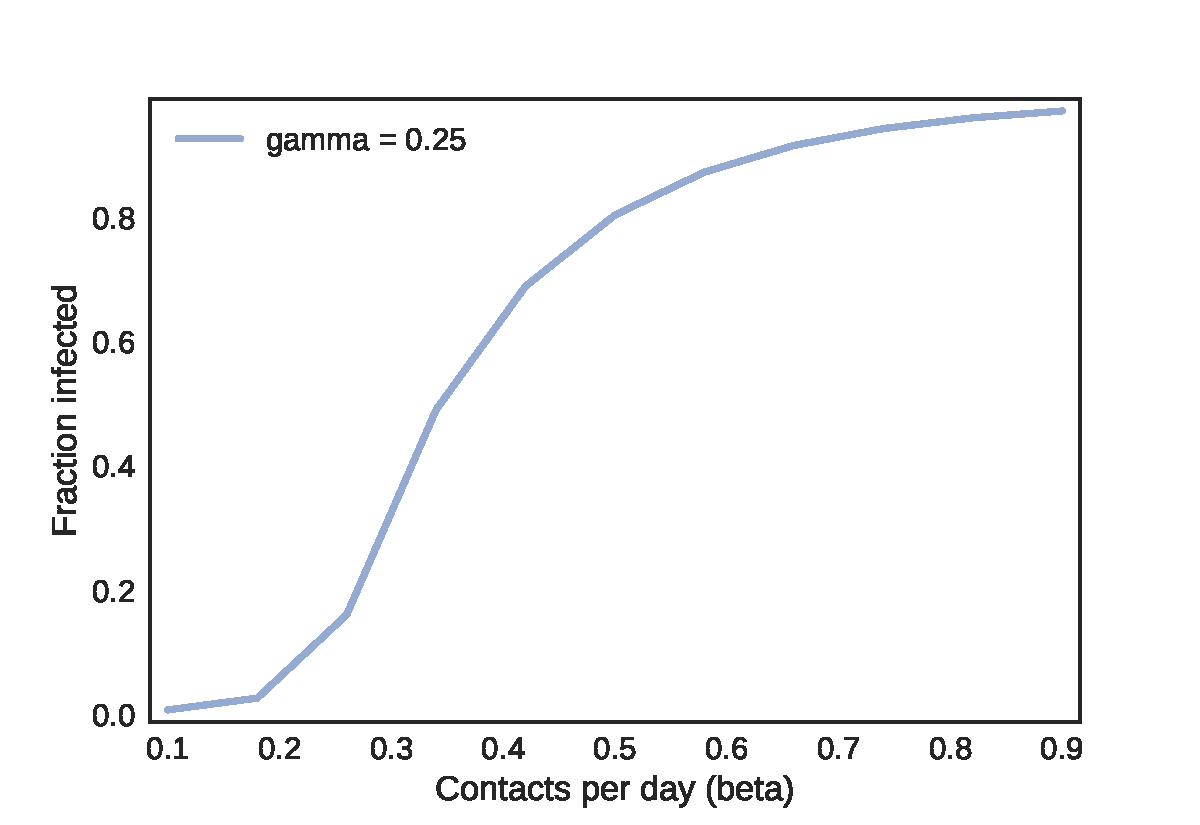
\includegraphics[height=3in]{figs/chap06-fig01.pdf}}
\caption{Total number of infected students as a function of the parameter \py{beta}, with \py{gamma = 0.25}.}
\label{chap06-fig01}
\end{figure}

Figure~\ref{chap06-fig01} shows the results.  Remember that this figure is a parameter sweep, not a time series, so the x-axis is the parameter \py{beta}, not time.  

When \py{beta} is small, the contact rate is low and the outbreak never really takes off; the total number of infected students is near zero.  As \py{beta} increases, it reaches a threshold near 0.3 where the fraction of infected students increases quickly.  When \py{beta} exceeds 0.5, more than 80\% of the population gets sick.


\section{Sweeping gamma}

Now let's see what that looks like for a few different values of \py{gamma}.  Again, we'll use \py{linspace} to make an array of values:
\index{linspace}

\begin{python}
gamma_array = linspace(0.1, 0.7, 4)
\end{python}

And run \py{sweep_beta} for each value of \py{gamma}:

\begin{python}
for gamma in gamma_array:
    infected_sweep = sweep_beta(beta_array, gamma)
    label = 'gamma = ' + str(gamma)
    plot(infected_sweep, label=label)
\end{python}

\begin{figure}
\centerline{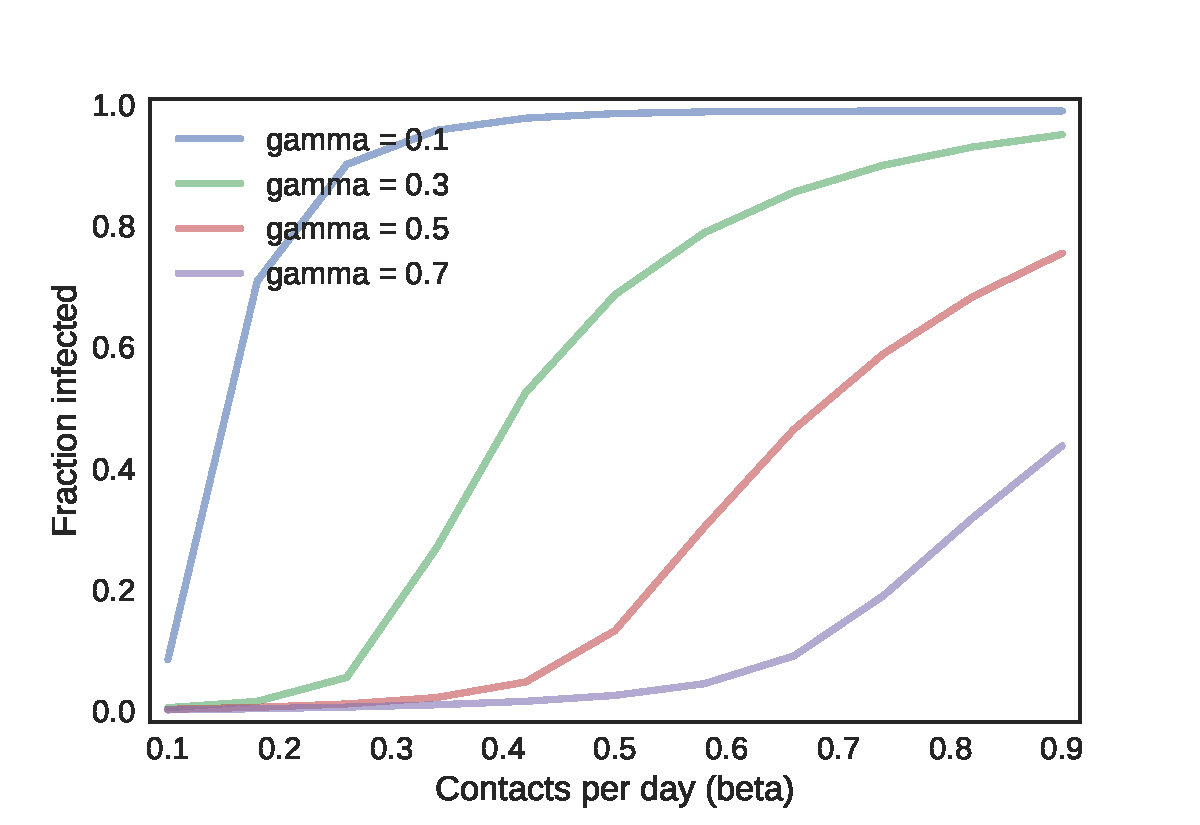
\includegraphics[height=3in]{figs/chap06-fig02.pdf}}
\caption{Total number of infected students as a function of the parameter \py{beta}, for several values of \py{gamma}.}
\label{chap06-fig02}
\end{figure}

Figure~\ref{chap06-fig02} shows the results.  When \py{gamma} is low, the recovery rate is low, which means people are infectious longer.  In that case, even low a contact rate (\py{beta}) results in an epidemic.

When \py{gamma} is high, \py{beta} has to be even higher to get things going.  That observation suggests that there might be a relationship between \py{gamma} and \py{beta} that determines the outcome of the model.  In fact, there is.  I will demonstrate it first by running simulations, then derive it by analysis.


\section{Nondimensionalization}
\label{nondim}

Before we go on, let's wrap the code from the previous section in a function:

\begin{python}
def sweep_parameters(beta_array, gamma_array):
    frame = SweepFrame(columns=gamma_array)
    for gamma in gamma_array:
        frame[gamma] = sweep_beta(beta_array, gamma)
    return frame
\end{python}

\py{sweep_parameters} takes as parameters two arrays: a range of values for \py{beta} and a range of values for \py{gamma}.

It creates a \py{SweepFrame} to store the results, with one column for each value of \py{gamma} and one row for each value of \py{beta}.  A \py{SweepFrame} is a kind of \py{DataFrame}, defined in the \py{modsim} library.  Its purpose is to store results from a two-dimensional parameter sweep.
\index{SweepFrame object}
\index{DataFrame object}

Each time through the loop, we run \py{sweep_beta}.  The result is a \py{SweepSeries} object with one element for each value of \py{gamma}.  The assignment

\begin{python}
frame[gamma] = sweep_beta(beta_array, gamma)
\end{python}

stores the values from the \py{SweepSeries} object as a new column in the \py{SweepFrame}, corresponding to the current value of \py{gamma}.

At the end, the \py{SweepFrame} stores the fraction of students infected for each pair of parameters, \py{beta} and \py{gamma}.

We can run \py{sweep_parameters} like this:

\begin{python}
frame = sweep_parameters(beta_array, gamma_array)
\end{python}

Then we can loop through the results like this:

\begin{python}
for gamma in frame.columns:
    series = frame[gamma]
    for beta in series.index:
        frac_infected = series[beta]
        print(beta, gamma, frac_infected)
\end{python}

This is the first example we've seen with one \py{for} loop inside another:

\begin{itemize}

\item Each time the outer loop runs, it selects a value of \py{gamma} from the columns of the \py{DataFrame} and extracts the corresponding column as a \py{Series}.
\index{Series}

\item Each time the inner loop runs, it selects a value of \py{beta} from the \py{Series} and selects the corresponding element, which is the fraction of student infected.

\end{itemize}  

In this example, \py{frame} has 4 columns, one for each value of \py{gamma}, and 11 rows, one for each value of \py{beta}.  So these loops print 44 lines, one for each pair of parameters.

Now let's think about possible relationships between \py{beta} and \py{gamma}:

\begin{itemize}

\item When \py{beta} exceeds \py{gamma}, that means there are more contacts (that is, potential infections) than recoveries.  The difference between \py{beta} and \py{gamma} might be called the ``excess contact rate", in units of contacts per day.

\item As an alternative, we might consider the ratio \py{beta/gamma}, which is the number of contacts per recovery.  Because the numerator and denominator are in the same units, this ratio is {\bf dimensionless}, which means it has no units.
\index{dimensionless}

\end{itemize}

Describing physical systems using dimensionless parameters is often a useful move in the modeling and simulation game.  It is so useful, in fact, that it has a name: {\bf nondimensionalization} (see \url{http://modsimpy.com/nondim}).
\index{nondimensionalization}

So we'll try the second option first.  In the notebook for this chapter, you can explore the first option as an exercise.

The following function wraps the previous loops and plots the fraction infected as a function of the ratio \py{beta/gamma}:

\begin{python}
def plot_sweep_frame(frame):
    for gamma in frame.columns:
        series = frame[gamma]
        for beta in series.index:
            frac_infected = series[beta]
            plot(beta/gamma, frac_infected, 'ro')
\end{python}

\begin{figure}
\centerline{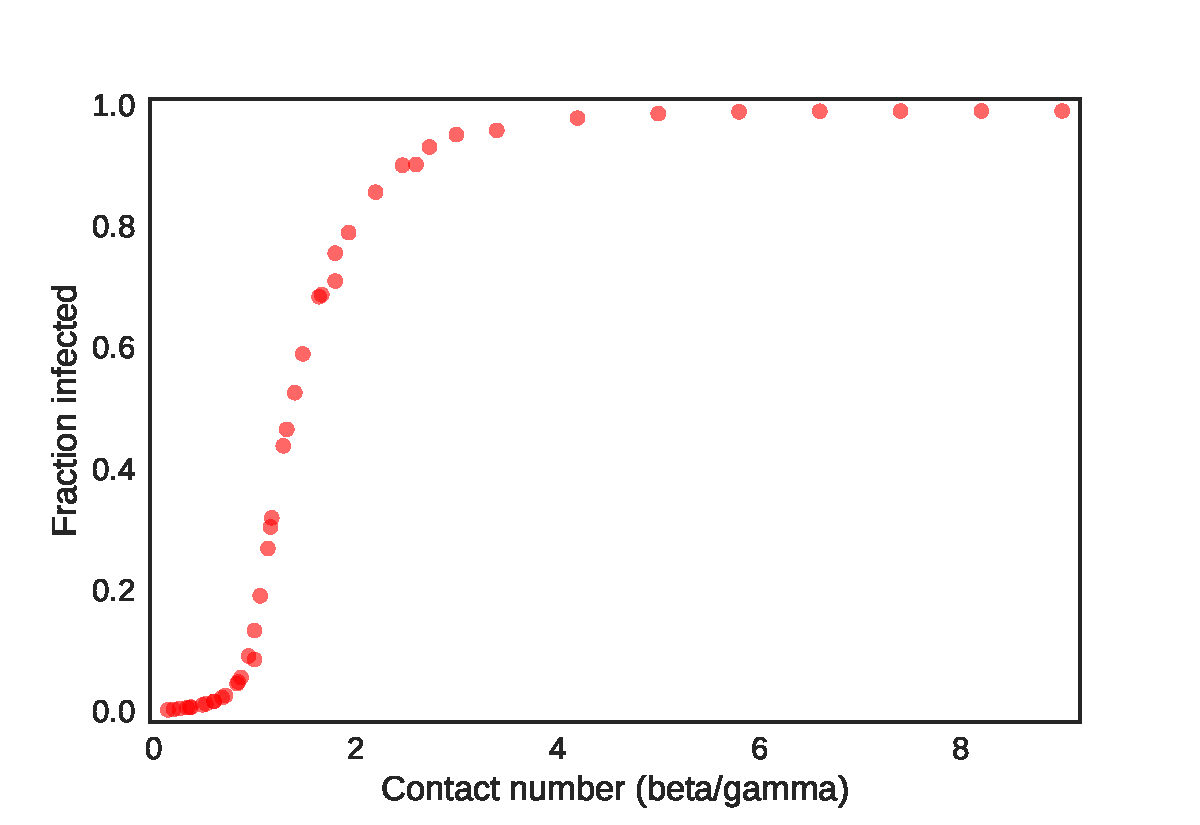
\includegraphics[height=3in]{figs/chap06-fig03.pdf}}
\caption{Total fraction infected as a function of contact number.}
\label{chap06-fig03}
\end{figure}

Figure~\ref{chap06-fig03} shows that the results fall neatly on a single curve, at least approximately.  That means that we can predict the fraction of students who will be infected based on a single parameter, the ratio \py{beta/gamma}.  We don't need to know the values of \py{beta} and \py{gamma} separately.


\section{Contact number}
\label{contact}

Recall that the number of new infections in a given day is $\beta s i N$, and the number of recoveries is $\gamma i N$.  If we divide these quantities, the result is $\beta s / \gamma$, which is the number of new infections per recovery (as a fraction of the population).
\index{contact number}
\index{basic reproduction number}

When a new disease is introduced to a susceptible population, $s$ is approximately 1, so the number of people infected by each sick person is $\beta / \gamma$.  This ratio is called the ``contact number" or ``basic reproduction number" (see \url{http://modsimpy.com/contact}).  By convention it is usually denoted $R_0$, but in the context of an SIR model, this notation is confusing, so we'll use $c$ instead.

The results in the previous section suggest that there is a relationship between $c$ and the total number of infections.  We can derive this relationship by analyzing the differential equations from Section~\ref{sireqn}:
%
\begin{align*}
\frac{ds}{dt} &= -\beta s i \\
\frac{di}{dt} &= \beta s i - \gamma i\\
\frac{dr}{dt} &= \gamma i
\end{align*}
%
In the same way we divided the contact rate by the infection rate to get the dimensionless quantity $c$, now we'll divide $di/dt$ by $ds/dt$ to get a ratio of rates:
%
\[ \frac{di}{ds} = -1 + \frac{1}{cs} \]
%
Dividing one differential equation by another is not an obvious move, but in this case it is useful because it gives us a relationship between $i$, $s$ and $c$ that does not depend on time.  We can multiply both sides of the equation by $ds$:
%
\[ di = \left( -1 + \frac{1}{cs} \right) ds \]
%
And then integrate both sides:
%
\[ i = -s + \frac{1}{c} \log s + q \]
%
where $q$ is a constant of integration.  Rearranging terms yields:
%
\[ q = i + s - \frac{1}{c} \log s \]
%
Now let's see if we can figure out what $q$ is.  At the beginning of an epidemic, if the fraction infected is small and nearly everyone is susceptible, we can use the approximations $i(0) = 0$ and $s(0) = 1$ to compute $q$:
%
\[ q = 0 + 1 + \frac{1}{c} \log 1 \]
%
Since $\log 1 = 0$, we get $q = 1$.
\index{integration}
\index{constant of integration}

\newcommand{\sinf}{s_{\infty}}

Now, at the end of the epidemic, let's assume that $i(\infty) = 0$ and $s(\infty)$ is an unknown quantity $\sinf$.  Now we have:
%
\[ q = 1 = 0 + \sinf - \frac{1}{c} \log \sinf \]
%
Solving for $c$, we get
%
\[ c = \frac{\log \sinf}{\sinf - 1} \]
%
If we create a range of values for $\sinf$
\index{linspace}

\begin{python}
s_inf_array = linspace(0.0001, 0.9999, 31)
\end{python}

we can compute the corresponding values of $c$:

\begin{python}
c_array = log(s_inf_array) / (s_inf_array - 1)
\end{python}

To get the total infected, we compute the difference between $s(0)$ and $s(\infty)$, then store the results in a \py{Series}:
\index{array}
\index{series}

\begin{python}
frac_infected = 1 - s_inf_array
frac_infected_series = Series(frac_infected, index=c_array)
\end{python}

Recall from Section~\ref{series} that a \py{Series} object contains an index and a corresponding sequence of values.  In this case, the index is \py{c_array} and the values are from \py{frac_infected}.


\section{Analysis and simulation}

Now we can plot the results:

\begin{python}
plot(frac_infected_series)
\end{python}

\begin{figure}
\centerline{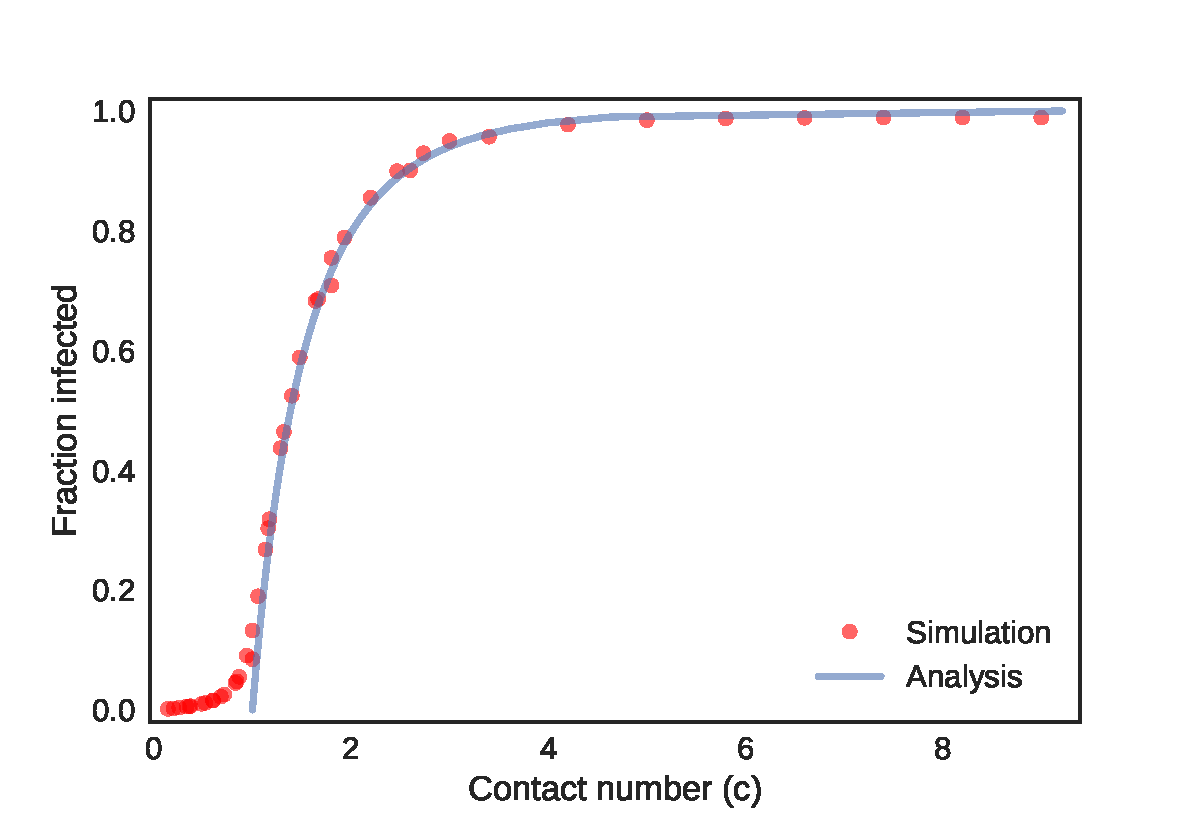
\includegraphics[height=3in]{figs/chap06-fig04.pdf}}
\caption{Total fraction infected as a function of contact number, showing results from simulation and analysis.}
\label{chap06-fig04}
\end{figure}

Figure~\ref{chap06-fig04} compares the analytic results from this section with the simulation results from Section~\ref{nondim}.  Over most of the range they are consistent with each other, with one discrepancy: when the contact number is less than 1, analysis indicates there should be no infections; but in the simulations a small part of the population is affected even when $c<1$.
\index{analysis}

The reason for the discrepancy is that the simulation divides time into a discrete series of days, whereas the analysis treats time as a continuous quantity.  In other words, the two methods are actually based on different models.  So which model is better?

Probably neither.  When the contact number is small, the early progress of the epidemic depends on details of the scenario.  If we are lucky, the original infected person, ``patient zero",  infects no one and there is no epidemic.  If we are unlucky, patient zero might have a large number of close friends, or might work in the dining hall (and fail to observe safe food handling procedures).
\index{patient zero}

For contact numbers near or less than 1, we might need a more detailed model.  But for higher contact numbers the SIR model might be good enough.

Figure~\ref{chap06-fig04} shows that if we know the contact number, we can compute the fraction infected.  But we can also read the figure the other way; that is, at the end of an epidemic, if we can estimate the fraction of the population that was ever infected, we can use it to estimate the contact number.

Well, at least in theory.  In practice, it might not work very well, because of the shape of the curve.  When the contact number is near 2, the curve is quite steep, which means that small changes in $c$ yield big changes in the number of infections.  If we observe that the total fraction infected is anywhere from 20\% to 80\%, we would conclude that $c$ is near 2.

On the other hand, for larger contact numbers, nearly the entire population is infected, so the curve is quite flat.  In that case we would not be able to estimate $c$ precisely, because any value greater than 3 would yield effectively the same results.  Fortunately, this is unlikely to happen in the real world; very few epidemics affect anything like 90\% of the population.

In summary, the SIR model has limitations; nevertheless, it provides insight into the behavior of infectious disease, especially the phenomenon of herd resistance.  As we saw in the previous chapter, if we know the parameters of the model, we can use it to evaluate possible interventions.  And as we saw in this chapter, we might be able to use data from earlier outbreaks to estimate the parameters.



\chapter{Thermal systems}

So far the systems we have studied have been physical, in the sense that they exist in the world, but they have not been physics, in the sense of what physics classes are usually about.  In this chapter, we'll do some physics, starting with {\bf thermal systems}, that is, systems where the temperature of objects changes as heat transfers from one to another.
\index{thermal system}

You can view the code for this chapter at \url{http://modsimpy.com/chap07}.  For instructions for downloading and running the code, see Section~\ref{code}.

\section{The coffee cooling problem}

The coffee cooling problem was discussed by Jearl Walker in {\it Scientific American} in 1977\footnote{Walker, ``The Amateur Scientist", {\it Scientific American}, Volume 237, Issue 5, November 1977.}; since then it has become a standard example of modeling and simulation.
\index{coffee cooling problem}
\index{Walker, Jearl}

Here is my version of the problem:

\begin{quote}
Suppose I stop on the way to work to pick up a cup of coffee, which I take with milk.  Assuming that I want the coffee to be as hot as possible when I arrive at work, should I add the milk at the coffee shop, wait until I get to work, or add the milk at some point in between?
\end{quote}

To help answer this question, I made a trial run with the milk and coffee in separate containers and took some measurements:

\begin{itemize}

\item When served, the temperature of the coffee is \SI{90}{\celsius}.  The volume is \SI{300}{mL}.

\item The milk is at an initial temperature of \SI{5}{\celsius}, and I take about \SI{50}{mL}.

\item The ambient temperature in my car is \SI{22}{\celsius}.

\item The coffee is served in a well insulated cup.  When I arrive at work after 30 minutes, the temperature of the coffee has fallen to \SI{70}{\celsius}.

\item The milk container is not as well insulated.  After 15 minutes, it warms up to \SI{20}{\celsius}, nearly the ambient temperature.

\end{itemize}

To use this data and answer the question, we have to know something about temperature and heat, and we have to make some modeling decisions.
\index{data}

\section{Temperature and heat}

To understand how coffee cools (and milk warms), we need a model of temperature and heat.  {\bf Temperature} is a property of an object or a system; in SI units it is measured in degrees Celsius (\si{\celsius}).  Temperature quantifies how hot or cold the object is, which is related to the average velocity of the particles that make up the object.
\index{temperature}

When particles in a hot object contact particles in a cold object, the hot object gets cooler and the cold object gets warmer, as energy is transferred from one to the other.  The transferred energy is called {\bf heat}; in SI units it is measured in joules (\si{\joule}).
\index{heat}

Heat is related to temperature by the following equation (see \url{http://modsimpy.com/thermass}):
%
\[ Q = C \Delta T \]
%
where $Q$ is the amount of heat transferred to an object, $\Delta T$ is resulting change in temperature, and $C$ is the {\bf thermal mass} of the object, which quantifies how much energy it takes to heat or cool it.  In SI units, thermal mass is measured in joules per degree Celsius (\si{\joule\per\celsius}).
\index{thermal mass}

For objects made primarily from one material, thermal mass can be computed like this:
%
\[ C = m c_p \]
%
where $m$ is the mass of the object and $c_p$ is the {\bf specific heat capacity} of the material (see \url{http://modsimpy.com/specheat}).
\index{specific heat capacity}

We can use these equations to estimate the thermal mass of a cup of coffee.  The specific heat capacity of coffee is probably close to that of water, which is \SI{4.2}{\joule\per\gram\per\celsius}.  Assuming that the density of coffee is close to that of water, which is \SI{1}{\gram\per\milli\liter}, the mass of \SI{300}{\milli\liter} of coffee is \SI{300}{\gram}, and the thermal mass is \SI{1260}{\joule\per\celsius}.
\index{density}

So when a cup of coffee cools from \SI{90}{\celsius} to \SI{70}{\celsius}, the change in temperature, $\Delta T$ is \SI{20}{\celsius}, which means that \SI{25200}{\joule} of heat energy was transferred from the coffee to the surrounding environment (the cup holder and air in my car).

To give you a sense of how much energy that is, if you were able to harness all of that heat to do work (which you cannot\footnote{See \url{http://modsimpy.com/thermo}.}), you could use it to lift a cup of coffee from sea level to \SI{8571}{\meter}, just shy of the height of Mount Everest, \SI{8848}{\meter}.
\index{Mount Everest}

Assuming that the cup has less mass than the coffee, and is made from a material with lower a specific heat, we can ignore the thermal mass of the cup.


\section{Heat transfer}

In a situation like the coffee cooling problem, there are three ways heat transfers from one object to another (see \url{http://modsimpy.com/transfer}):
\index{heat transfer}
\index{conduction}
\index{convection}
\index{radiation}

\begin{itemize}

\item Conduction: When objects at different temperatures come into contact, the faster-moving particles of the higher-temperature object transfer kinetic energy to the slower-moving particles of the lower-temperature object.

\item Convection: When particles in a gas or liquid flow from place to place, they carry heat energy with them.  Fluid flows can be caused by external action, like stirring, or by internal differences in temperature.  For example, you might have heard that hot air rises, which is a form of ``natural convection".
\index{fluid flow}

\item Radiation: As the particles in an object move due to thermal energy, they emit electromagnetic radiation.  The energy carried by this radiation depends on the object's temperature and surface properties (see \url{http://modsimpy.com/thermrad}).

\end{itemize}

For objects like coffee in a car, thermal radiation is much smaller than 
heat transfer due to conduction and convection, so we will ignore it.

Convection can be a complex topic, since it often depends on details of fluid flow in three dimensions.  But for this problem we will be able to get away with a simple model called ``Newton's law of cooling".
\index{Newton's law of cooling}

\section{Newton's law of cooling}

Newton's law of cooling asserts that the temperature rate of change for an object is proportional to the difference in temperature between the object and the surrounding environment:
%
\[ \frac{dT}{dt} = -r (T - T_{env}) \]
%
where $T$, the temperature of the object, is a function of time, $t$; $T_{env}$ is the temperature of the environment, and $r$ is a constant that characterizes how quickly heats is transferred between the system and the environment.

Newton's so-called ``law" is really a model in the sense that it is approximately true in some conditions, only roughly true in others, and not at all true in others.

For example, if the primary mechanism of heat transfer is conduction, Newton's law is ``true", which is to say that $r$ is constant over a wide range of temperatures.  And sometimes we can estimate $r$ based on the material properties and shape of the object.

When convection contributes a non-negligible fraction of heat transfer, $r$  depends on temperature, but Newton's law is often accurate enough, at least over a narrow range of temperatures.  In this case $r$ usually has to be estimated experimentally, since it depends on details of surface shape, air flow, evaporation, etc.

When radiation makes up a substantial part of heat transfer, Newton's law is not a good model at all.  This is the case for objects in space or in a vacuum, and for objects at high temperatures (more than a few hundred degrees Celsius, say).
\index{radiation}

However, for a situation like the coffee cooling problem, we expect Newton's model to be quite good.


\section{Implementation}
\label{coffee_impl}

To get started, let's forget about the milk temporarily and focus on the coffee.  I'll create a \py{State} object to represent the initial temperature:

\begin{python}
init = State(temp=90)
\end{python}

And a \py{System} object to contain the parameters of the system:
\index{State object}
\index{System object}

\begin{python}
coffee = System(init=init, T_env=22, r=0.01,
                t0=0, t_end=30, dt=1)
\end{python}

The values of \py{T_env}, \py{t0}, and \py{t_end} come from the statement of the problem.  I chose the value of \py{r} arbitrarily for now; we will figure out how to estimate it soon.
\index{time step}

\py{dt} is the time step we use to simulate the cooling process.
Strictly speaking, Newton's law is a differential equation, but over a short period of time we can approximate it with a difference equation:
%
\[ \Delta T = -r (T - T_{env}) \Delta t \]
%
where $\Delta t$ is a small time step and $\Delta T$ is the change in temperature during that time step.

Note: I use $\Delta T$ to denote a change in temperature over time, but in the context of heat transfer, you might also see $\Delta T$ used to denote the difference in temperature between an object and its environment, $T - T_{env}$.  To minimize confusion, I avoid this second use.

Now we can write an update function:
\index{unpack}

\begin{python}
def update(state, system):
    unpack(system)
    
    T = state.temp
    T += -r * (T - T_env) * dt

    return State(temp=T)
\end{python}

Now if we run 

\begin{python}
update(init, coffee)
\end{python}

we see that the temperature after one minute is \SI{89.3}{\celsius}, so the temperature drops by about \SI{0.7}{\celsius\per\minute}, at least for this value of \py{r}.

Now we can use \py{run_simulation}, as defined in Section~\ref{timeframe}, to simulate a series of time steps from \py{t0} to \py{t_end}:
\index{time step}
\index{\py{run_simulation}}
\index{unpack}

\begin{python}
def run_simulation(system, update_func):
    unpack(system)
    
    frame = TimeFrame(columns=init.index)
    frame.loc[t0] = init
    ts = linrange(t0, t_end-dt, dt)
    
    for t in ts:
        frame.loc[t+dt] = update_func(frame.loc[t], system)
    
    system.results = frame
\end{python}

and run it like this:

\begin{python}
run_simulation(coffee, update)
\end{python}

The result is a \py{TimeFrame} object with one row per time step and just one column, \py{temp}.  The temperature after 30 minutes is \SI{72.3}{\celsius}, which is a little higher than stated in the problem, \SI{70}{\celsius}.  We could adjust \py{r} by hand and find the right value by trial and error, but we can do better, as we'll see in the next section.
\index{time step}
\index{TimeFrame object}

First I want to wrap what we have so far in a function:

\begin{python}
def make_system(T_init=90, r=0.01, volume=300, t_end=30):
    init = State(temp=T_init)
    
    system = System(init=init,
                    volume=volume,
                    r=r,
                    T_env=22, 
                    t0=0,
                    t_end=t_end,
                    dt=1)
    return system
\end{python}

\py{make_system} takes the system parameters and packs them into a \py{System} object.  Now we can simulate the coffee like this:
\index{\py{make_system}}

\begin{python}
coffee = make_system()
run_simulation(coffee, update)
\end{python}

Now let's see a better was to estimate \py{r}.


\section{Using fsolve}
\label{fsolve}

SciPy provides a method called \py{fsolve} that finds the roots of non-linear equations.  As a simple example, suppose you want to find the roots of the polynomial
%
\[ f(x) = (x - 1)(x - 2)(x - 3) \]
%
where {\bf root} means a value of $x$ that makes $f(x)=0$.  Because of the way I wrote the polynomial, we can see that if $x=1$, the first factor is 0; if $x=2$, the second factor is 0; and if $x=3$, the third factor is 0, so those are the roots.
\index{root}
\index{fsolve}

But usually it's not that easy.  In that case \py{fsolve} can help.  First, we have to write a function that evaluates $f$:

\begin{python}
def func(x):
    return (x-1) * (x-2) * (x-3)
\end{python}

Now we call \py{fsolve} like this:

\begin{python}
fsolve(func, x0=0)
\end{python}

The first argument is the function whose roots we want.  The second argument, \py{x0}, is an initial guess about where a root might be.  Generally, the closer the initial guess is to an actual root, the faster \py{fsolve} runs.  In this case, with the initial guess \py{x0=0}, the result is 1.

Often \py{fsolve} finds the root that's closest to the initial guess.  In this example, when \py{x0=1.9}, \py{fsolve} returns 2, and when \py{x0=2.9}, \py{fsolve} returns 3.  But this behavior can be unpredictable; with \py{x0=1.5}, \py{fsolve} returns 3.

So how can we use \py{fsolve} to estimate \py{r}?  

Now, we want to find the value of \py{r} that yields a final temperature of \SI{70}{\celsius}.  To work with \py{fsolve}, we need a function that takes \py{r} as a parameter and returns the difference between the final temperature and the goal:

\begin{python}
def error_func1(r):
    system = make_system(r=r)
    run_simulation(system, update)
    return final_temp(system) - 70
\end{python}

I call a function like this an ``error function" because it returns the difference between what we got and what we wanted, that is, the error.  When we find the right value of \py{r}, this error will be 0.
\index{error function}
\index{function!error}

We can test \py{error_func1} like this, using our initial guess for \py{r}:

\begin{python}
error_func1(r=0.01)
\end{python}

The result is an error of \SI{2.3}{\celsius}, because the final temperature with this value of \py{r} is too high.

Now we can call \py{fsolve} like this:

\begin{python}
solution = fsolve(error_func1, 0.01)
r_coffee = solution[0]
\end{python}

The return value from \py{fsolve} is an array with a single element, which is the root \py{fsolve} found.  In this example, \py{r_coffee} turns out to be about \py{0.012}, in units of \si{\per\minute}.

\begin{figure}
\centerline{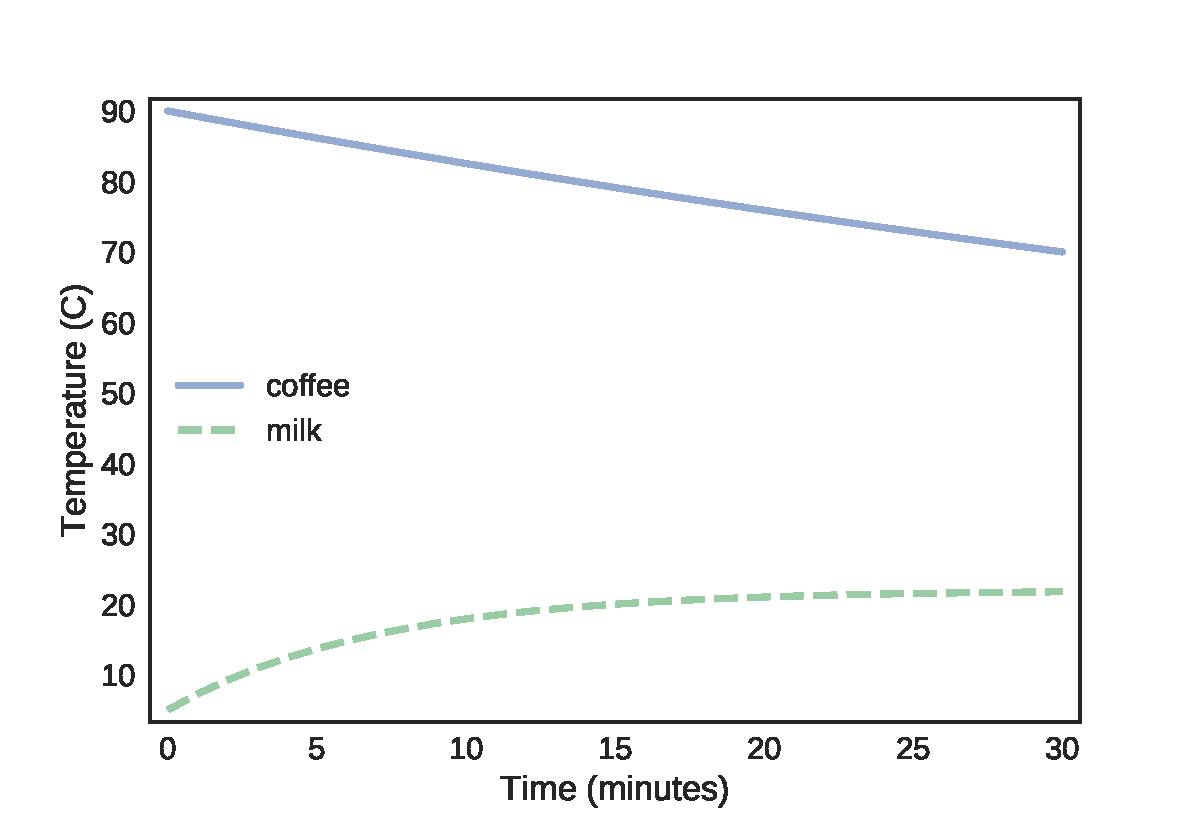
\includegraphics[height=3in]{figs/chap07-fig01.pdf}}
\caption{Temperature of the coffee and milk over time.}
\label{chap07-fig01}
\end{figure}

As one of the exercises for this chapter, you will use the same process to estimate \py{r_milk}.  

With the correct values of \py{r_coffee} and \py{r_milk}, the simulation results should look like Figure~\ref{chap07-fig01}, which shows the temperature of the coffee and milk over time.


\section{Mixing liquids}

When we mix two liquids, the temperature of the mixture depends on the temperatures of the ingredients, but it might not be obvious how to compute it.
\index{mixing}

Assuming there are no chemical reactions between the liquids that either produce or consume heat, the total thermal energy of the system is the same before and after mixing; in other words, thermal energy is {\bf conserved}.
\index{conservation of energy}

If the temperature of the first liquid is $T_1$, the temperature of the second liquid is $T_2$, and the final temperature of the mixture is $T$, the heat transfer into the first liquid is $C_1 (T - T_1)$ and the heat transfer into the second liquid is $C_2 (T - T_2)$, where $C_1$ and $C_2$ are the thermal masses of the liquids.

In order to conserve energy, these heat transfers must add up to 0:
%
\[ C_1 (T - T_1) + C_2 (T - T_2) = 0 \]
%
We can solve this equation for T:
%
\[ T = \frac{C_1 T_1 + C_2 T_2}{C_1 + C_2} \]
%
For the coffee cooling problem, we have the volume of each liquid; if we also know the density, $\rho$, and the specific heat capacity, $c_p$, we can compute thermal mass:
%
\[ C = \rho V c_p \]
%
If we assume that the density and specific heat of the milk and coffee are equal, they drop out of the equation, and we can write:
%
\[ T = \frac{V_1 T_1 + V_2 T_2}{V_1 + V_2} \]
%
where $V_1$ and $V_2$ are the volumes of the liquids.  As an exercise, you can look up the density and specific heat of milk to see how good this approximation is.
\index{volume}
\index{density}
\index{specific heat}

The following function takes two \py{System} objects that represent the coffee and milk, and creates a new \py{System} to represent the mixture:

\begin{python}
def mix(s1, s2):
    assert s1.t_end == s2.t_end
    
    volume = s1.volume + s2.volume
    
    temp = (s1.volume * final_temp(s1) + 
            s2.volume * final_temp(s2)) / volume
    
    mixture = make_system(T_init=temp,
                          volume=volume,
                          r=s1.r)
    
    return mixture
\end{python}

The first line is an \py{assert} statement, which is a way of checking for errors.  It compares \py{t_end} for the two systems to confirm that they have been cooling for the same time.  If not, \py{assert} displays an error message and stops the program.
\index{assert statement}
\index{statement!assert}

The next two statements compute the total volume of the mixture and its temperature.  Fianlly, \py{mix} makes a new \py{System} object and returns it.

This function uses the value of \py{r} from \py{s1} as the value of \py{r} for the mixture.  If \py{s1} represents the coffee, and we are adding the milk to the coffee, this is probably a reasonable choice.  On the other hand, when we increase the amount of liquid in the coffee cup, that might change \py{r}.  So this is an assumption to we might want to revisit when.


\section{Mix first or last?}

Now we have everything we need to solve the problem.  First I'll create objects to represent the coffee and cream, and run for 30 minutes.

\begin{python}
coffee = make_system(T_init=90, t_end=30, 
                     r=r_coffee, volume=300)
run_simulation(coffee, update)

milk = make_system(T_init=5, t_end=30, 
                   r=r_milk, volume=50)
run_simulation(milk, update)
\end{python}

The final temperatures, before mixing, are \SI{70}{\celsius} and \SI{21.7}{\celsius}.  Then we mix them:

\begin{python}
mix_last = mix(coffee, milk)
\end{python}

After mixing, the temperature is \SI{63.1}{\celsius}, which is still warm enough to be enjoyable.  Would we do any better if we added the milk first?

To find out, I'll create new objects for the coffee and milk:

\begin{python}
coffee = run(T_init=90, r=r_coffee, volume=300)
milk = run(T_init=5, r=r_milk, volume=50)
\end{python}

Then mix them and simulate 30 minutes:

\begin{python}
mix_first = mix(coffee, milk)
mix_first.t_end = 30
run_simulation(mix_first, update)
\end{python}

The final temperature is only \SI{61.6}{\celsius}.  So it looks like adding the milk at the end is better, by about \SI{1.5}{\celsius}.  But is that the best we can do?


\section{Optimization}

Adding the milk after 30 minutes is better than adding immediately, but maybe there's something in between that's even better.  To find out, I'll use the following function, which takes \py{t_add} as a parameter:
\index{optimization}

\begin{python}
def run_and_mix(t_add, t_total=30):
    coffee = make_system(T_init=90, t_end=t_add, 
                         r=r_coffee, volume=300)
    run_simulation(coffee, update)

    milk = make_system(T_init=5, t_end=t_add, 
                       r=r_milk, volume=50)
    run_simulation(milk, update)
    
    mixture = mix(coffee, milk)
    mixture.t_end = t_total - t_add
    run_simulation(mixture, update)

    return final_temp(mixture)
\end{python}

When \py{t_add=0}, we add the milk immediately; when \py{t_add=30}, we add it at the end.  Now we can sweep the range of values in between:

\begin{python}
sweep = SweepSeries()
for t_add in linrange(0, 30, 2):
    temp = run_and_mix(t_add)
    sweep[t_add] = temp
\end{python}

\begin{figure}
\centerline{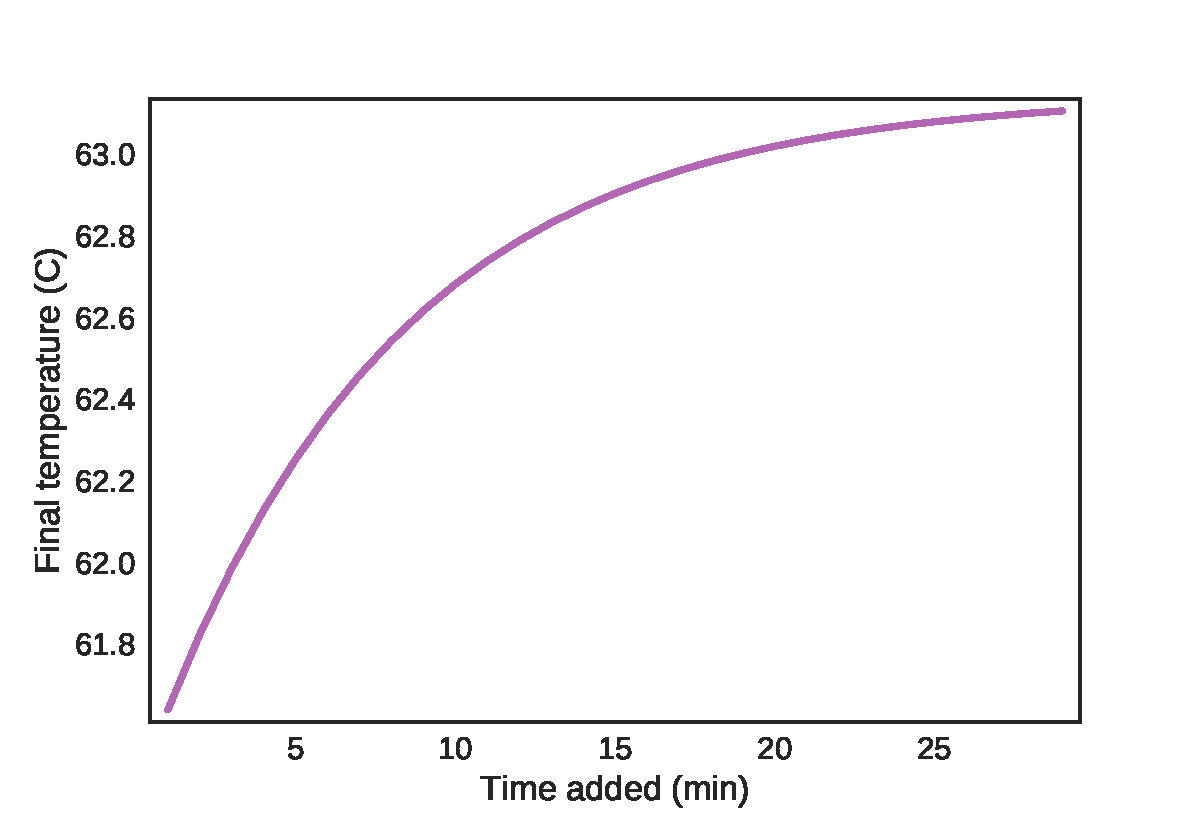
\includegraphics[height=3in]{figs/chap07-fig02.pdf}}
\caption{Final temperature as a function of the time the milk is added.}
\label{chap07-fig02}
\end{figure}

Figure~\ref{chap07-fig02} shows the result.  Again, note that this is a parameter sweep, not a time series.  The x-axis is the time when we add the milk, not the index of a \py{TimeSeries}.

The final temperature is maximized when \py{t_add=30}, so adding the milk at the end is optimal.

In the notebook for this chapter you will have a chance to explore this solution and try some variations.  For example, suppose the coffee shop won't let me take milk in a separate container, but I keep a bottle of milk in the refrigerator at my office.  In that case is it better to add the milk at the coffee shop, or wait until I get to the office?


\section{Analysis}

Simulating Newton's law of cooling is almost silly, because we can solve the differential equation analytically.  If
%
\[ \frac{dT}{dt} = -r (T - T_{env}) \]
%
the general solution is
%
\[ T{\left (t \right )} = C_{1} \exp(-r t) + T_{env} \]
%
and the particular solution where $T(0) = T_init$ is
%
\[ T_{env} + \left(- T_{env} + T_{init}\right) \exp(-r t) \]
%
You can see how I got this solution using SymPy at \url{http://modsimpy.com/sympy07}; if you would like to see it done by hand, you can watch this video: \url{http://modsimpy.com/khan3}.
\index{analysis}
\index{SymPy}

Now we can use the observed data to estimate the parameter $r$.  If we observe $T(t_{end}) = T_{end}$, we can plug $t_{end}$ and $T_{end}$ into the particular solution and solve for $r$.  The result is:
%
\[ r = \frac{1}{t_{end}} \log{\left (\frac{T_{init} - T_{env}}{T_{end} - T_{env}} \right )} \]
%
Plugging in $t_{end}=30$ and $T_{end}=70$ (and again with $T_{init}=90$ and $T_{env}=22$), the estimate for $r$ is 0.0116.

We can use the following function to compute the time series:
\index{unpack}

\begin{python}
def run_analysis(system):
    unpack(system)
    
    T_init = init.temp    
    ts = linrange(t0, t_end, dt)
    
    temp_array = T_env + (T_init - T_env) * exp(-r * ts)
    temp_series = TimeSeries(temp_array, index=ts)
    
    system.results = TimeFrame(temp_series, columns=['temp'])
\end{python}

This function is similar to \py{run_simulation}; it takes a \py{System} as a parameter, and stores a \py{TimeFrame} as a result.  We can run it like this, with \py{r_coffee2=0.0116}:
\index{\py{run_analysis}}

\begin{python}
init = State(temp=90)
coffee2 = System(init=init, T_env=22, r=r_coffee2, 
                 t0=0, t_end=30)
run_analysis(coffee2)
\end{python}

The final temperature is \SI{70}{\celsius}, as it should be.  In fact, the results are identical to what we got by simulation, with very small differences due to round off errors.


\chapter{Pharmacokinetics}

{\bf Pharmacokinetics} is the study of how drugs and other substances move around the body, react, and are eliminated.  In this chapter, we will implement one of the most widely used pharmacokinetic models: the so-called {\bf minimal model} of glucose and insulin in the blood stream.
\index{pharmacokinetics}

We will use this model to fit data collected from a patient, and use the parameters of the fitted model to quantify the patient's ability to produce insulin and process glucose.
\index{glucose}
\index{insulin}

My presentation in this chapter follows Bergman (2005) ``Minimal Model" (abstract at \url{http://modsimpy.com/bergman},
PDF at \url{http://modsimpy.com/minmod}).

You can view the code for this chapter at \url{http://modsimpy.com/chap08}.  For instructions for downloading and running the code, see Section~\ref{code}.


\section{The glucose-insulin system}

{\bf Glucose} is a form of sugar that circulates in the blood of animals; it is used as fuel for muscles, the brain, and other organs.  The concentration of blood sugar is controlled by the hormone system, and especially by {\bf insulin}, which is produced by the pancreas and has the effect of reducing blood sugar.
\index{pancreas}

In people with normal pancreatic function, the hormone system maintains {\bf homeostasis}; that is, it keeps the concentration of blood sugar in a range that is neither too high or too low.

But if the pancreas does not produce enough insulin, or if the cells that should respond to insulin become insensitive, blood sugar can become elevated, a condition called {\bf hyperglycemia}.  Long term, severe hyperglycemia is the defining symptom of {\bf diabetes mellitus}, a serious disease that affects almost 10\% of the population in the U.S. (see \url{http://modsimpy.com/cdc}).
\index{hyperglycemia}
\index{diabetes}

One of the most-used tests for hyperglycemia and diabetes is the frequently sampled intravenous glucose tolerance test (FSIGT), in which glucose is injected into the blood stream of a fasting subject (someone who has not eaten recently), and then blood samples are collected at intervals of 2--10 minutes for 3 hours.  The samples are analyzed to measure the concentrations of glucose and insulin.
\index{FSIGT}

By analyzing these measurements, we can estimate several parameters of the subject's response; the most important is a parameter denoted $S_I$, which quantifies the effect of insulin on the rate of reduction in blood sugar.


\section{The glucose minimal model}

The ``minimal model" was proposed by Bergman, Ider, Bowden, and Cobelli\footnote{Bergman RN, Ider YZ, Bowden CR, Cobelli C., ``Quantitative estimation of insulin sensitivity", Am J Physiol. 1979 Jun;236(6):E667-77.  Abstract at \url{http://modsimpy.com/insulin}.}.
It consists of two parts: the glucose model and the insulin model.  I will present an implementation of the glucose model; in the notebook for this chapter, you will have the chance to implement the insulin model.
\index{minimal model}

The original model was developed in the 1970s; since then, many variations and extensions have been proposed.  Bergman's comments on the development of the model provide insight into their process:

\begin{quote}
We applied the principle of Occam's Razor, i.e.~by asking
what was the simplest model based upon known physiology
that could account for the insulin-glucose relationship
revealed in the data. Such a model must be simple
enough to account totally for the measured glucose (given
the insulin input), yet it must be possible, using mathematical
techniques, to estimate all the characteristic parameters
of the model from a single data set (thus avoiding
unverifiable assumptions).
\end{quote}

The most useful models are the ones that achieve this balance: including enough realism to capture the essential features of the system without too much complexity to be practical.  In this case the practical limit is the ability to estimate the parameters of the model using data, and to interpret the parameters meaningfully.
\index{Occam's Razor}

Bergman discusses the features he and his colleagues thought were essential:

\begin{quote}
(1) Glucose, once elevated by injection, returns to basal level due to
two effects: the effect of glucose itself to normalize its own
concentration [...] as well as the catalytic effect of insulin to allow
glucose to self-normalize (2) Also, we discovered
that the effect of insulin on net glucose disappearance
must be sluggish --- that is, that insulin acts slowly because
insulin must first move from plasma to a remote compartment [...] to exert its action on glucose disposal.
\end{quote}

To paraphrase the second point, the effect of insulin on glucose disposal, as seen in the data, happens more slowly than we would expect if it depended primarily on the the concentration of insulin in the blood.  Bergman's group hypothesized that insulin must move, relatively slowly, from the blood to a ``remote compartment" where it has its effect.
\index{compartment model}

At the time, the remote compartment was a modeling abstraction that might, or might not, reflect something physical.  Later, according to Bergman, it was ``shown to be interstitial fluid", that is, the fluid that surrounds tissue cells.  In the history of mathematical modeling, it is common for hypothetical entities, added to models to achieve particular effects, to be found later to correspond to physical entities.
\index{interstitial fluid}

The glucose model consists of two differential equations:
%
\[ \frac{dG}{dt} = -k_1 \left[ G(t) - G_b \right] - X(t) G(t)  \]
%
\[ \frac{dX}{dt} = k_3 \left[I(t) - I_b \right] - k_2 X(t) \]
%
where

\begin{itemize}

\item $G$ is the concentration of blood glucose as a function of time and $dG/dt$ is its rate of change.

\item $I$ is the concentration of insulin in the blood as a function of time, which is taken as an input into the model, based on measurements.

\item $G_b$ is the basal concentration of blood glucose and $I_b$ is the basal concentration of blood insulin, that is, the concentrations at equilibrium.  Both are constants estimated from measurements at the beginning or end of the test.

\item $X$ is the concentration of insulin in the tissue fluid as a function of time, and $dX/dt$ is its rate of change.

\item $k_1$, $k_2$, and $k_3$ are positive-valued parameters that control the rates of appearance and disappearance for glucose and insulin. 

\end{itemize}

We can interpret the terms in the equations one by one:

\begin{itemize}

\item $-k_1 \left[ G(t) - G_b \right]$ is the rate of glucose disappearance due to the effect of glucose itself.  When $G(t)$ is above basal level, $G_b$, this term is negative; when $G(t)$ is below basal level this term is positive.  So in the absence of insulin, this term tends to restore blood glucose to basal level.

\item $-X(t) G(t)$ models the interaction of glucose and insulin in tissue fluid, so the rate increases as either $X$ or $G$ increases.  This term does not require a rate parameter because the units of $X$ are unspecified; we can consider $X$ to be in whatever units would make the parameter of this term 1.

\item $k_3 \left[ I(t) - I_b \right]$ is the rate at which insulin diffuses between blood and tissue fluid.  When $I(t)$ is above basal level, insulin diffuses from the blood into the tissue fluid.  When $I(t)$ is below basal level, insulin diffuses from tissue to the blood.

\item $-k_2 X(t)$ is the rate of insulin disappearance in tissue fluid as it is consumed or broken down.

\end{itemize}

The initial state of the model is $X(0) = I_b$ and $G(0) = G_0$, where $G_0$ is a constant that represents the concentration of blood sugar immediately after the injection.  In theory we could estimate $G_0$ based on measurements, but in practice it takes time for the injected glucose to spread through the blood volume.  Since $G_0$ is not measurable, it is treated as a {\bf free parameter} of the model, which means that we are free to choose it to fit the data.
\index{free parameter}


\section{Data}

To develop and test the model, I'll use data from Pacini and Bergman\footnote{``MINMOD: A computer program to calculate insulin sensitivity and pancreatic responsivity from the frequently sampled intravenous glucose tolerance test", {\em Computer Methods and Programs in Biomedicine} 23: 113-122, 1986.}.  The dataset is in a file in the repository for this book, which we can read into a \py{DataFrame}:
\index{data}
\index{DataFrame object}

\begin{python}
data = pd.read_csv('glucose_insulin.csv', index_col='time')
\end{python}

\py{data} has two columns: \py{glucose} is the concentration of blood glucose in \si{\milli\gram/\deci\liter}; \py{insulin} is concentration of insulin in the blood in \si{\micro U\per\milli\liter} (a medical ``unit", denoted \si{U}, is an amount defined by convention in context).  The index is time in \si{\minute}.
\index{concentration}

\begin{figure}
\centerline{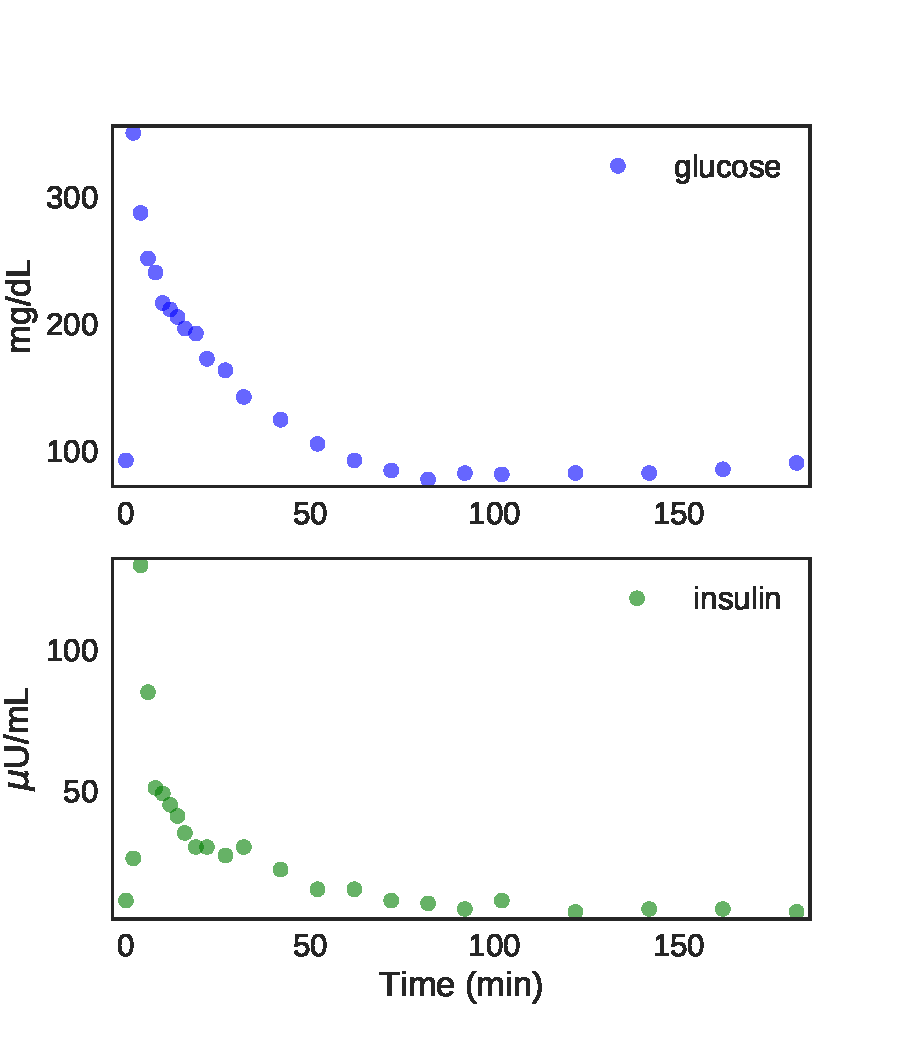
\includegraphics[width=3in]{figs/chap08-fig01.pdf}}
\caption{Glucose and insulin concentrations measured by FSIGT.}
\label{chap08-fig01}
\end{figure}

Figure~\ref{chap08-fig01} shows glucose and insulin concentrations over \SI{182}{\minute} for a subject with normal insulin production and sensitivity.


\section{Interpolation}
\label{interpolate}

Before we are ready to implement the model, there's one problem we have to solve.  In the differential equations, $I$ is a function that can be evaluated at any time, $t$.  But in the \py{DataFrame}, we only have measurements at discrete times.  This is a job for interpolation!
\index{interpolation}

The \py{modsim} library provides a function named \py{interpolate}, which is a wrapper for the SciPy function \py{interp1d}.  It takes any kind of \py{Series} as a parameter, including \py{TimeSeries} and \py{SweepSeries}, and returns a function.  That's right, I said it returns a {\em function}.
\index{function!as return value}
\index{Series}
\index{interpolate}
\index{interp1d}
\index{SciPy}

So we can call \py{interpolate} like this:

\begin{python}
I = interpolate(data.insulin)
\end{python}

Then we can call the new function, \py{I}, like this:

\begin{python}
I(18)
\end{python}

The result is 31.66, which is a linear interpolation between the actual measurements at \py{t=16} and \py{t=19}.  We can also pass an array as an argument to \py{I}:

\begin{python}
ts = linrange(0, 182, 2)
I(ts)
\end{python}

The result is an array of interpolated values for equally-spaced values of \py{t} between 0 and 182.
\index{linrange}

\py{interpolate} can take additional arguments, which it passes along to \py{interp1d}.  You can read about these options at \url{http://modsimpy.com/interp}.


\section{Implementation}
\label{glucose}

To get started, we'll assume that the parameters of the model are known.  We'll implement the model and use it to generate time series for \py{G} and \py{X}.  Then we'll see how to find parameter values that generate series that best fit the data.

Taking advantage of estimates from prior work, I'll start with these values:

\begin{python}
k1 = 0.03
k2 = 0.02
k3 = 1e-05
G0 = 290
\end{python}

And I'll use the measurements at \py{t=0} as the basal levels:

\begin{python}
Gb = data.glucose[0]
Ib = data.insulin[0]
\end{python}

Now we can create the initial state:
\index{State object}
\index{System object}

\begin{python}
init = State(G=G0, X=0)
\end{python}

And the \py{System} object:

\begin{python}
system = System(init=init, 
                k1=k1, k2=k2, k3=k3,
                I=I, Gb=Gb, Ib=Ib,
                t0=0, t_end=182, dt=2)
\end{python}

Now here's the update function:
\index{update function}
\index{function!update}

\begin{python}
def update_func(state, t, system):
    G, X = state
    unpack(system)
        
    dGdt = -k1 * (G - Gb) - X*G
    dXdt = k3 * (I(t) - Ib) - k2 * X
    
    G += dGdt * dt
    X += dXdt * dt

    return State(G=G, X=X)
\end{python}

As usual, the update function takes a \py{State} object and a \py{System} as parameters, but there's  one difference from previous examples: this update function also takes \py{t}.  That's because this system of differential equations is {\bf time dependent}; that is, time appears in the right-hand side of at least one equation.
\index{time dependent}

The first line of \py{update} uses multiple assignment to extract the current values of \py{G} and \py{X}.  The second line uses \py{unpack} so we can read the system variables without using the dot operator.
\index{unpack}

Computing the derivatives \py{dGdt} and \py{dXdt} is straightforward; we just have to translate the equations from math notation to Python.
\index{derivative}

Then, to perform the update, we multiply each derivative by the discrete time step \py{dt}, which is \SI{2}{\minute} in this example.  The return value is a \py{State} object with the new values of \py{G} and \py{X}.
\index{time step}

Before running the simulation, it is always a good idea to run the update function with the initial conditions:

\begin{python}
update_func(init, 0, system)
\end{python}

If there are no errors, and the results seem reasonable, we are ready to run the simulation.  Here's one more version of \py{run_simulation}.  It is almost the same as in Section~\ref{coffee_impl}, with one change: it passes \py{t} as an argument to \py{update_func}.
\index{\py{run_simulation}}
\index{unpack}

\begin{python}
def run_simulation(system, update_func):
    unpack(system)
    
    frame = TimeFrame(columns=init.index)
    frame.loc[t0] = init
    ts = linrange(t0, t_end-dt, dt)
    
    for t in ts:
        frame.loc[t+dt] = update_func(frame.loc[t], t, system)
    
    system.results = frame
\end{python}

And we can run it like this:

\begin{python}
run_simulation(system, update_func)
\end{python}

\begin{figure}
\centerline{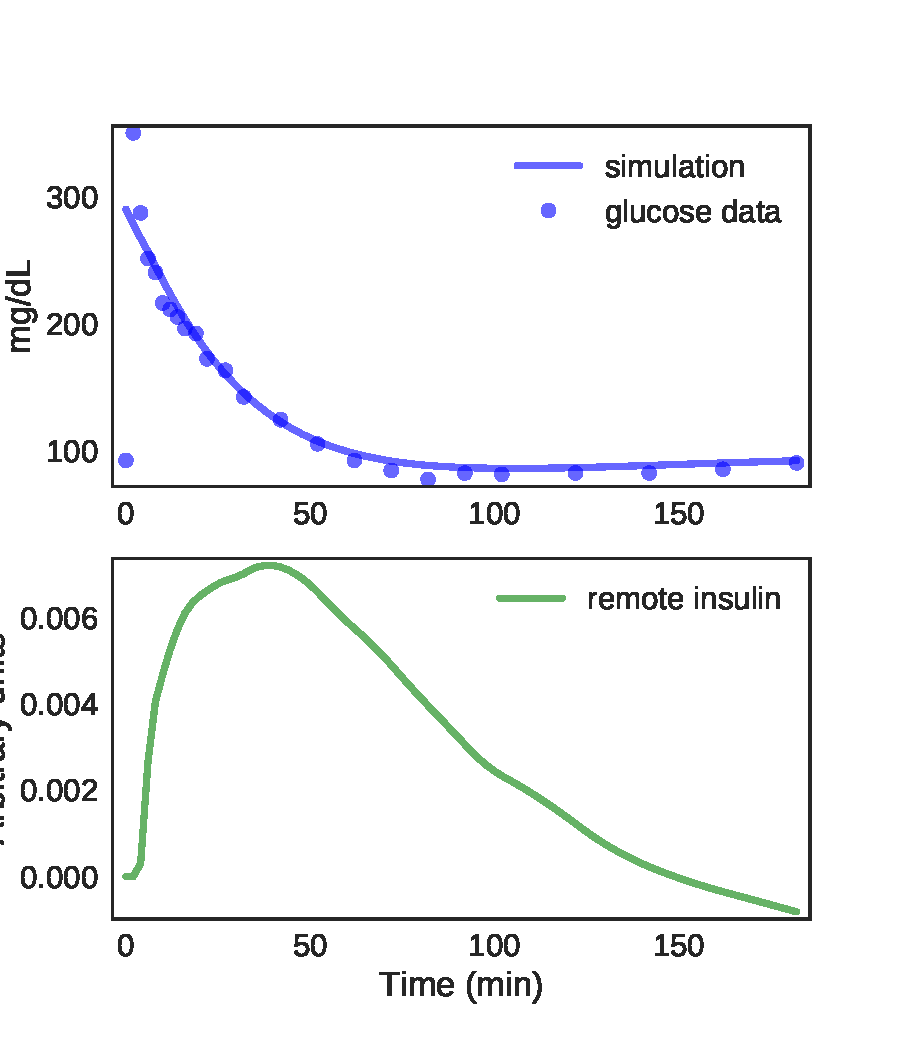
\includegraphics[width=3in]{figs/chap08-fig03.pdf}}
\caption{Results from simulation of the glucose minimal model.}
\label{chap08-fig03}
\end{figure}

The results are shown in Figure~\ref{chap08-fig03}.  The top plot shows simulated glucose levels from the model along with the measured data.  The bottom plot shows simulated insulin levels in tissue fluid, which is in unspecified units, and not to be confused with measured concentration of insulin in the blood.

With the parameters I chose, the model fits the data reasonably well.  We can do better, but first, I want to replace \py{run_simulation} with a better differential equation solver.
\index{fitting data}
\index{quality of fit}


\section{Numerical solution of differential equations}
\label{slopefunc}

So far we have been solving differential equations by rewriting them as difference equations.  In the current example, the differential equations are:
%
\[ \frac{dG}{dt} = -k_1 \left[ G(t) - G_b \right] - X(t) G(t)  \]
%
\[ \frac{dX}{dt} = k_3 \left[I(t) - I_b \right] - k_2 X(t) \]
%
If we multiply both sides by $dt$, we have:
%
\[ dG = \left[ -k_1 \left[ G(t) - G_b \right] - X(t) G(t) \right] dt  \]
%
\[ dX = \left[ k_3 \left[I(t) - I_b \right] - k_2 X(t) \right] dt \]
%
When $dt$ is very small, or more precisely {\bf infinitesimal}, this equation is exact.  But in our simulations, $dt$ is \SI{2}{\minute}, which is small but not infinitesimal.  In effect, the simulations assume that the derivatives $dG/dt$ and $dX/dt$ are constant during each \SI{2}{\minute} time step.  That's not exactly true, but it can be a good enough approximation.
\index{time step}

This method, evaluating derivatives at discrete time steps and assuming that they are constant in between, is called {\bf Euler's method} (see \url{http://modsimpy.com/euler}).
\index{Euler's method}

Euler's method is good enough for some simple problems, but there are many better ways to solve differential equations, including an entire family of methods called linear multistep methods (see \url{http://modsimpy.com/lmm}).
\index{linear multistep method}

Rather than implement these methods ourselves, we will use functions from SciPy.  The \py{modsim} library provides a function called \py{run_odeint}, which is a wrapper for \py{scipy.integrate.odeint}.  The name \py{odeint} stands for ``ordinary differential equation integrator".  The equations we are solving are ``ordinary'' because all the derivatives are with respect to the same variable; in other words, there are no partial derivatives.  And the solver is called an integrator because solving differential equations is considered a form of integration.
\index{ordinary differential equation}
\index{odeint}
\index{LSODA}
\index{ODEPACK}

\py{scipy.integrate.odeint} is a wrapper for \py{LSODA}, which is from ODEPACK, a venerable collection of ODE solvers written in Fortran (for some of the history of ODEPACK, see \url{http://modsimpy.com/hindmarsh}).

To use \py{odeint}, we have to provide a ``slope function":
\index{slope function}
\index{function!slope}
\index{unpack}

\begin{python}
def slope_func(state, t, system):
    G, X = state
    unpack(system)
    
    dGdt = -k1 * (G - Gb) - X*G
    dXdt = k3 * (I(t) - Ib) - k2 * X
    
    return dGdt, dXdt
\end{python}

\py{slope_func} is similar to \py{update_func}; in fact, it takes the same parameters in the same order.  But \py{slope_func} is simpler, because all we have to do is compute the derivatives, that is, the slopes.  We don't have to do the updates; \py{odeint} does them for us.

Before we call \py{run_odeint}, we have to create a \py{System} object:
\index{System object}

\begin{python}
system2 = System(init=init, 
                k1=k1, k2=k2, k3=k3,
                I=I, Gb=Gb, Ib=Ib,
                ts=data.index)
\end{python}

When we were using \py{run_simulation}, we created a \py{System} object with variables \py{t0}, \py{t_end}, and \py{dt}.  When we use \py{run_odeint}, we don't need those variables, but we do have to provide \py{ts}, which is an array or \py{Series} that contains the times where we want the solver to evaluate $G$ and $X$.
\index{\py{run_odeint}}

Now we can call \py{run_odeint} like this:

\begin{python}
run_odeint(system2, slope_func)
\end{python}

Like \py{run_simulation}, \py{run_odeint} puts the results in a \py{TimeFrame} and stores it as a system variable named \py{results}.  The columns of \py{results} match the state variables in \py{init}, \py{G} and \py{X}.  The index of \py{results} matches the values from \py{ts}; in this example, \py{ts} contains the timestamps of the measurements.
\index{TimeFrame object}

The results are similar to what we saw in Figure~\ref{chap08-fig03}.  The difference is about 1\% on average and never more than 2\%.


\section{Least squares}

So far we have been taking the parameters as given, but in general we don't have that luxury.  Normally we are given the data and we have to search for the parameters that yield a time series that best matches the data.
\index{fitting data}

We will do that now, in two steps:

\begin{enumerate}

\item First we'll define an {\bf error function} that takes a set of possible parameters, simulates the system with the given parameters, and computes the errors, that is, the differences between the simulation results and the data.
\index{error function}
\index{function~error}

\item Then we'll use a SciPy function, \py{leastsq}, to search for the parameters that minimize mean squared error (MSE).
\index{leastsq}
\index{mean squared error}
\index{MSE}

\end{enumerate}

Here's an outline of the functions we'll use:

\begin{itemize}

\item The \py{modsim} library provides \py{fit_leastsq}, which takes a function called \py{error_func} as a parameter.  It does some error-checking, then calls \py{scipy.optimize.leastsq}, which does the real work.
\index{\py{fit_leastsq}}

\item \py{scipy.optimize.leastsq} uses functions called \py{lmdif} and \py{lmdir}, which implement the Levenberg-Marquardt algorithm for non-linear least squares problems (see \url{http://modsimpy.com/levmarq}).  These functions are provided by another venerable FORTRAN library called MINPACK (see \url{http://modsimpy.com/minpack}).
\index{SciPy}
\index{lmdif}
\index{MINPACK}

\item When \py{scipy.optimize.leastsq} runs, it calls \py{error_func} many times, each time with a different set of parameters, until it converges on the set of parameters that minimizes MSE.
\index{\py{error_func}}

\end{itemize}

Each time the error function runs, it creates a \py{System} object with the given parameters, so let's wrap that operation in a function:
\index{\py{make_system}}
\index{System object}

\begin{python}
def make_system(G0, k1, k2, k3, data):
    init = State(G=G0, X=0)
    system = System(init=init, 
                    k1=k1, k2=k2, k3=k3,
                    Gb=Gb, Ib=Ib, 
                    I=interpolate(data.insulin),
                    ts=data.index)
    return system
\end{python}

\py{make_system} takes \py{G0} and the rate constants as parameters, as well as \py{data}, which is the \py{DataFrame} containing the measurements.  It creates and returns a \py{System} object.

Now here's the error function:

\begin{python}
def error_func(params, data):
    system = make_system(*params, data)
    run_odeint(system, slope_func)
    error = system.results.G - data.glucose
    return error
\end{python}

The parameters of \py{error_func} are

\begin{itemize}

\item \py{params}, which is a sequence of four system parameters, and

\item \py{data}, which is the \py{DataFrame} containing the measurements.

\end{itemize}

\py{error_func} uses \py{make_system} to create the \py{System} object.  This line demonstrates a feature we have not seen before, the {\bf scatter operator}, \py{*}.  Applied to \py{params}, the scatter operator unpacks the sequence, so instead of being considered a single value, it is treated as four separate values.
\index{scatter operator}
\index{operator!scatter}

\py{error_func} calls \py{run_odeint} using the same slope function we saw in Section~\ref{slopefunc}.  Then it computes the difference between the simulation results and the data.  Since \py{system.results.G} and \py{data.glucose} are both \py{Series} objects, the result of subtraction is also a \py{Series}.
\index{Series}
\index{\py{run_odeint}}

Now, to do the actual minimization, we run \py{fit_leastsq}:

\begin{python}
k1 = 0.03
k2 = 0.02
k3 = 1e-05
G0 = 290
params = G0, k1, k2, k3
best_params = fit_leastsq(error_func, params, data)
\end{python}

\py{error_func} is the function we just defined.  \py{params} is a sequence containing an initial guess for the four system parameters, and \py{data} is the \py{DataFrame} containing the measurements.
\index{\py{fit_leastsq}}

Actually, the third parameter can be any object we like.  \py{fit_leastsq} and \py{leastsq} don't do anything with this parameter except to pass it along to \py{error_func}, so in general it contains whatever information \py{error_func} needs to do its job.


\section{Interpreting parameters}

The return value from \py{fit_leastsq} is \py{best_params}, which we can pass along to \py{make_system}, again using the scatter operator, and then run the simulation:

\begin{python}
system = make_system(*best_params, data)
run_odeint(system, slope_func)
\end{python}

\begin{figure}
\centerline{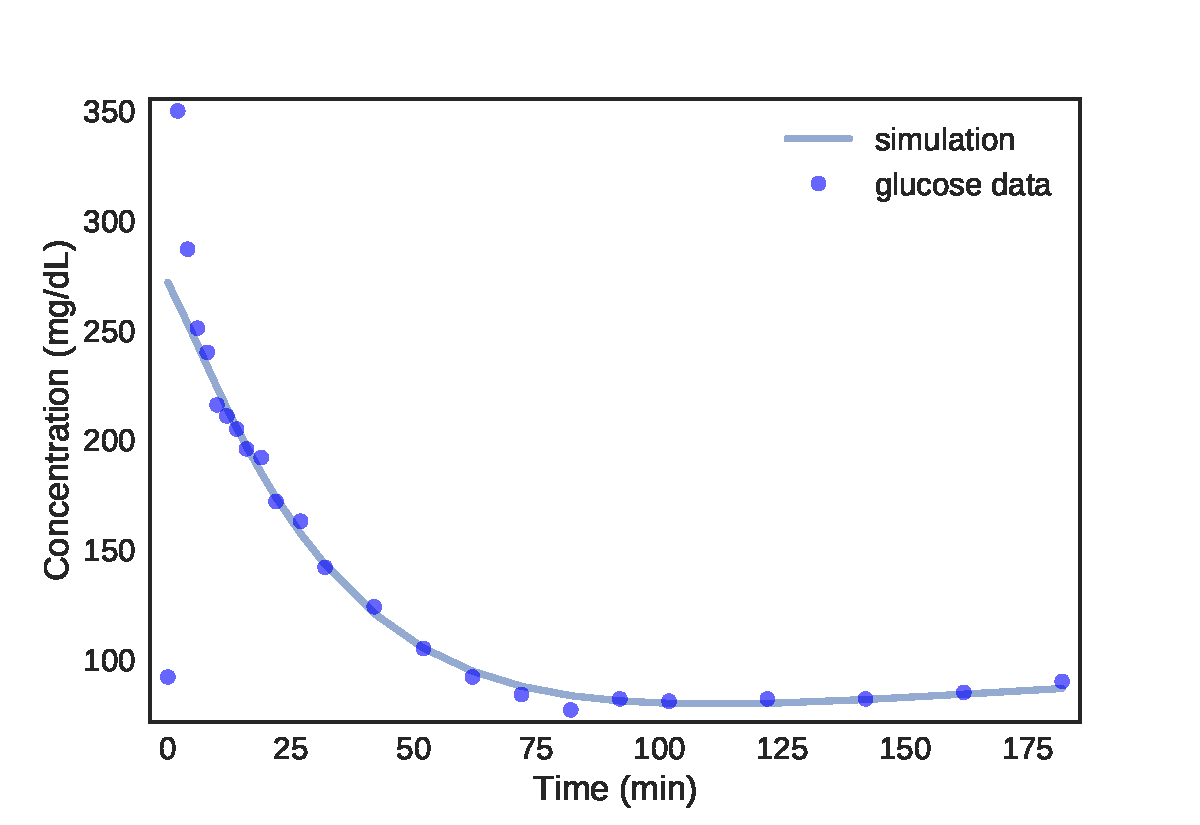
\includegraphics[height=3in]{figs/chap08-fig04.pdf}}
\caption{Simulation of the glucose minimal model with parameters that minimize MSE.}
\label{chap08-fig04}
\end{figure}

Figure~\ref{chap08-fig04} shows the results.  The simulation matches the measurements well, except during the first few minutes after the injection.  But we don't expect the model to do well in this regime.

The reason is that the model is {\bf non-spatial}; that is, it does not take into account different concentrations in different parts of the body.  Instead, it assumes that the concentrations of glucose and insulin in blood, and insulin in tissue fluid, are the same throughout the body.  This way of representing the body is known among experts as the ``bag of blood" model.
\index{non-spatial model}
\index{bag of blood}

Immediately after injection, it takes time for the injected glucose to circulate.  During that time, we don't expect a non-spatial model to be accurate.  For this reason, we should not take the estimated value of \py{G0} too seriously; it is useful for fitting the model, but not meant to correspond to a physical, measurable quantity.

On the other hand, the other parameters are meaningful; in fact, they are the reason the model is useful.  Using the best-fit parameters, we can estimate two quantities of interest:
\index{glucose effectiveness}
\index{insulin sensitivity}

\begin{itemize}

\item ``Glucose effectiveness", $E$, which is the tendency of elevated glucose to cause depletion of glucose.  

\item ``Insulin sensitivity", $S$, which is the ability of elevated blood insulin to enhance glucose effectiveness.

\end{itemize}

Glucose effectiveness is defined as the change in $dG/dt$ as we vary $G$:
%
\[ E \equiv - \frac{\delta \dot{G}}{\delta G} \]
%
where $\dot{G}$ is shorthand for $dG/dt$.  Taking the derivative of $dG/dt$ with respect to $G$, we get
%
\[ E = k_1 + X \]
%
The {\bf glucose effectiveness index}, $S_G$, is the value of $E$ in when blood insulin is near its basal level, $I_b$.  In that case, $X$ approaches 0 and $E$ approaches $k_1$.  So we can use the best-fit value of $k_1$ as an estimate of $S_G$.
\index{basal level}

Insulin sensitivity is defined as the change in $E$ as we vary $I$:
%
\[ S \equiv - \frac{\delta E}{\delta I} \]
%
The {\bf insulin sensitivity index}, $S_I$, is the value of $S$ when $E$ and $I$ are at steady state:
%
\[ S_I \equiv \frac{\delta E_{SS}}{\delta I_{SS}} \]
%
$E$ and $I$ are at steady state when $dG/dt$ and $dX/dt$ are 0, but we don't actually have to solve those equations to find $S_I$.  If we set $dX/dt = 0$ and solve for $X$, we find the relation:
%
\[ X_{SS} = \frac{k_3}{k_2} I_{SS} \]
%
And since $E = k_1 + X$, we have:
%
\[ S_I = \frac{\delta E_{SS}}{\delta I_{SS}} = \frac{\delta X_{SS}}{\delta I_{SS}} \]
%
Taking the derivative of $X_{SS}$ with respect to $I_{SS}$, we have:
%
\[ S_I = k_3 / k_2 \]
%
So if we find parameters that make the model fit the data, we can use $k_3 / k_2$ as an estimate of $S_I$.  

For the example data, the estimated values of $S_G$ and $S_I$ are $0.029$ and for $8.9 \times 10^{-4}$.  According to Pacini and Bergman, these values are within the normal range.


\section{The insulin minimal model}

Along with the glucose minimal mode, Berman et al.~developed an insulin minimal model, in which the concentration of insulin, $I$, is governed by this differential equation:
%
\[ \frac{dI}{dt} = -k I(t) + \gamma \left[ G(t) - G_T \right] t \]
%
where

\begin{itemize}

\item $k$ is a parameter that controls the rate of insulin disappearance independent of blood glucose.   

\item $G(t)$ is the measured concentration of blood glucose at time $t$.

\item $G_T$ is the glucose threshold; when blood glucose is above this level, it triggers an increase in blood insulin. 

\item $\gamma$ is a parameter that controls the rate of increase (or decrease) in blood insulin when glucose is above (or below) $G_T$.

% TODO: explain why t is there

\end{itemize}

The initial condition is $I(0) = I_0$.  As in the glucose minimal model, we treat the initial condition as a parameter which we'll choose to fit the data.
\index{insulin minimal model}
\index{differential equation}

The parameters of this model can be used to estimate, $\phi_1$ and $\phi_2$, which are values that ``describe the sensitivity to glucose of the first and second phase pancreatic responsivity".  They are related to the parameters as follows:
%
\[ \phi_1 = \frac{I_{max} - I_b}{k (G_0 - G_b)}\]
%
\[ \phi_2 = \gamma \times 10^4 \]
%
where $I_{max}$ is the maximum measured insulin level, and $I_b$ and $G_b$ are the basal levels of insulin and glucose.

In the notebook for this chapter, you will have a chance to implement this model, find the parameters that best fit the data, and estimate these values.


\chapter{Projectiles}

So far the differential equations we've worked with have been {\bf first order}, which means they involve only first derivatives.   In this chapter, we turn our attention to second order ODEs, which can involve both first and second derivatives.  
\index{first order ODE}
\index{second order ODE}

We'll revisit the falling penny example from Chapter~\ref{chap01}, and use \py{odeint} to find the position and velocity of the penny as it falls, with and without air resistance.

You can view the code for this chapter at \url{http://modsimpy.com/chap09}.  For instructions for downloading and running the code, see Section~\ref{code}.


\section{Newton's second law of motion}

First order ODEs can be written
%
\[ \frac{dy}{dx} = G(x, y) \]
%
where $G$ is some function of $x$ and $y$ (see \url{http://modsimpy.com/ode}).  Second order ODEs can be written
%
\[ \frac{d^2y}{dx^2} = H(x, y, y') \]
%
where $H$ is another function and $y'$ is shorthand for $dy/dx$.  In particular, we will work with one of the most famous and useful second order ODEs, Newton's second law of motion:
%
\[ F = m a \]
%
where $F$ is a force or the total of a set of forces, $m$ is the mass of a moving object, and $a$ is its acceleration.
\index{Newton's second law of motion}
\index{differential equation}
\index{acceleration}
\index{velocity}
\index{position}

Newton's law might not look like a differential equation, until we realize that acceleration, $a$, is the second derivative of position, $y$, with respect to time, $t$.  With the substitution
%
\[ a = \frac{d^2y}{dt^2} \]
%
Newton's law can be written
%
\[ \frac{d^2y}{dt^2} = F / m \]
%
And that's definitely a second order ODE.  In general, $F$ can be a function of time, position, and velocity.

Of course, this ``law" is really a model, in the sense that it is a simplification of the real world.  Although it is often approximately true:

\begin{itemize}

\item It only applies if $m$ is constant.  If mass depends on time, position, or velocity, we have to use a more general form of Newton's law (see \url{http://modsimpy.com/varmass}).
\index{variable mass}

\item It is not a good model for very small things, which are better described by another model, quantum mechanics.
\index{quantum mechanics}

\item And it is not a good model for things moving very fast, which are better described by relativistic mechanics.
\index{relativity}

\end{itemize}

But for medium to large things with constant mass, moving at speeds that are medium to slow, Newton's model is phenomenally useful.  If we can quantify the forces that act on such an object, we can figure out how it will move.


\section{Dropping pennies}

As a first example, let's get back to the penny falling from the Empire State Building, which we considered in Section~\ref{penny}.  We will implement two models of this system: first without air resistance, then with.
\index{falling penny}
\index{air resistance}

Given that the Empire State Building is \SI{381}{\meter} high, and assuming that the penny is dropped with velocity zero, the initial conditions are:
\index{State object}

\begin{python}
init = State(y=381 * m, 
             v=0 * m/s)
\end{python}

where \py{y} is height above the sidewalk and \py{v} is velocity.  The units \py{m} and \py{s} are from the \py{UNITS} object provided by Pint:
\index{unit}
\index{Pint}

\begin{python}
m = UNITS.meter
s = UNITS.second
kg = UNITS.kilogram
\end{python}

The only system parameter is the acceleration of gravity:

\begin{python}
g = 9.8 * m/s**2
\end{python}

In addition, we'll specify the sequence of times where we want to solve the differential equation:

\begin{python}
duration = 10 * s
dt = 1 * s
ts = linrange(0, duration, dt)
\end{python}

%TODO: check prior uses of arange, linspace, and linrange

\py{ts} contains equally spaced points between \SI{0}{\second} and \SI{10}{\second}, including both endpoints.
\index{linrange}

Next we need a \py{System} object to contain the system parameters:
\index{System object}

\begin{python}
system = System(init=init, g=g, ts=ts)
\end{python}

Now we need a slope function, and here's where things get tricky.  As we have seen, \py{odeint} can solve systems of first order ODEs, but Newton's law is a second order ODE.  However, if we recognize that
\index{slope function}
\index{function!slope}

\begin{enumerate}

\item Velocity, $v$, is the derivative of position, $dy/dt$, and

\item Acceleration, $a$, is the derivative of velocity, $dv/dt$,

\end{enumerate}

we can rewrite Newton's law as a system of first order ODEs:
%
\[ \frac{dy}{dt} = v \]
%
\[ \frac{dv}{dt} = a \]
%
And we can translate those equations into a slope function:
\index{system of equations}
\index{unpack}

\begin{python}
def slope_func(state, t, system):
    y, v = state
    unpack(system)    

    dydt = v
    dvdt = -g
    
    return dydt, dvdt
\end{python}

The first parameter, \py{state}, contains the position and velocity of the penny.  The last parameter, \py{system}, contains the system parameter \py{g}, which is the magnitude of acceleration due to gravity.
\index{State object}

The second parameter, \py{t}, is time.  It is not used in this slope function because none of the factors of the model are time dependent (see Section~\ref{glucose}).  I include it anyway because this function will be called by \py{odeint}, and \py{odeint} always provides the same arguments, whether they are needed or not.
\index{time dependent}

The rest of the function is a straightforward translation of the differential equations, with the substitution $a = -g$, which indicates that acceleration is due to gravity, in the direction of decreasing $y$.  \py{slope_func} returns a sequence containing the two derivatives.

Before calling \py{run_odeint}, it is always a good idea to test the slope function with the initial conditions:

\begin{python}
slope_func(init, 0, system)
\end{python}

The result is a sequence containing \SI{0}{\meter\per\second} for velocity and \SI{9.8}{\meter\per\second\squared} for acceleration.  Now we can run \py{odeint} like this:

\begin{python}
run_odeint(system, slope_func)
\end{python}

\py{run_odeint} stores the results in a \py{TimeFrame} with two columns: \py{y} contains the height of the penny; \py{v} contains its velocity.  
\index{TimeFrame object}
\index{\py{run_odeint}}

\py{plot_position}, which is defined in the notebook for this chapter, plots height versus time:

\begin{python}
plot_position(system.results)
\end{python}

\begin{figure}
\centerline{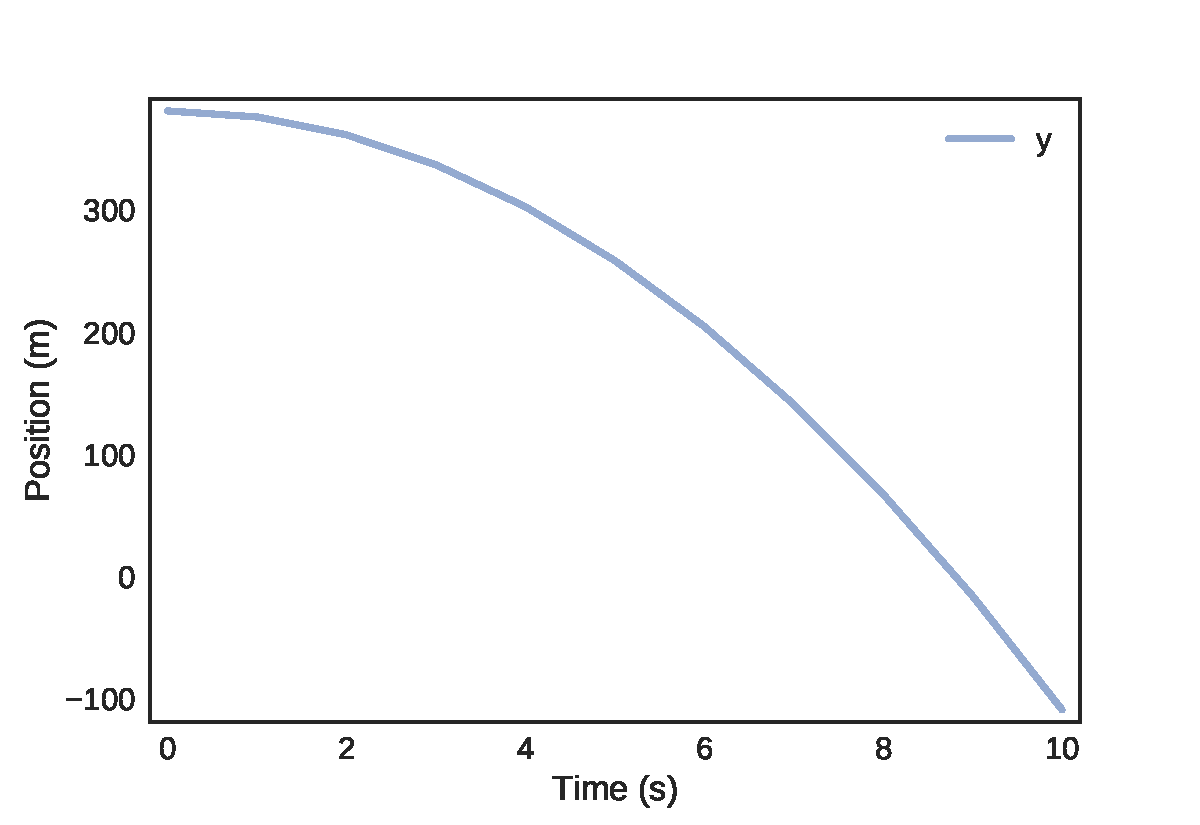
\includegraphics[height=3in]{figs/chap09-fig01.pdf}}
\caption{Height of the penny versus time, with no air resistance.}
\label{chap09-fig01}
\end{figure}

Figure~\ref{chap09-fig01} shows the result.  Since acceleration is constant, velocity increases linearly and position decreases quadratically; as a result, the height curve is a parabola.
\index{parabola}

In this model, height can be negative, because we have not included the effect of the sidewalk!


\section{Onto the sidewalk}
\label{sidewalk}

To avoid negative heights, we can use the results from the previous section to estimate when the penny hits the sidewalk, and run the simulation for the estimated time.

From the results, we can extract \py{y}, which is a \py{Series} that represents height as a function of time.

\begin{python}
y = system.results.y
\end{python}

To interpolate the values of \py{y}, we could use \py{interpolate}, which we saw in Section~\ref{interpolate}.

\begin{python}
Y = interpolate(y)
\end{python}

If we do that, we get a function that computes height as a function of time, but that's not what we want.  Rather, we want the inverse function, time as a function of height.   The \py{modsim} library provides a function that computes it:

\begin{python}
T = interp_inverse(y, kind='cubic')
\end{python}

The second parameter, \py{kind}, indicates what kind of interpolation we want: \py{cubic} means we want a cubic spline (see \url{http://modsimpy.com/spline}).
\index{interpolate}
\index{\py{interp_inverse}}
\index{cubic spline}
\index{spline}

The result is a function that maps from height to time.  Now we can evaluate the interpolating function at \py{y=0}

\begin{python}
T_sidewalk = T(0)
\end{python}

The result is \SI{8.8179}{\meter}, which agrees with the exact answer to 4 decimal places.

One caution about \py{interpolate} and \py{interp_inverse}: the function you provide has to be single valued (see \url{http://modsimpy.com/singval}).

In this example, height decreases monotonically, so for every height there is only one corresponding time.  But if we threw the penny upward and then it fell down, the penny would pass through some heights more than once.  In that case the inverse function represented by \py{T} would not be single valued, and the interpolation function would behave unpredictably.
\index{single valued}
\index{monotonic}


\section{With air resistance}
\label{drag}

As an object moves through a fluid, like air, the object applies force to the air and, in accordance with Newton's third law of motion, the air applies an equal and opposite force to the object (see \url{http://modsimpy.com/newton}).
\index{air resistance}
\index{drag force}
\index{force!drag}
\index{drag equation}

The direction of this {\bf drag force} is opposite the direction of travel, and its magnitude is given by the drag equation (see \url{http://modsimpy.com/drageq}):
%
\[ F_d = \frac{1}{2}~\rho~v^2~C_d~A \]
%
where

\begin{itemize}

\item $F_d$ is force due to drag, in newtons (\si{\newton}).

\item $\rho$ is the density of the fluid in \si{\kg\per\meter\cubed}.
\index{density}

\item $v$ is velocity in \si{\meter\per\second}.
\index{velocity}

\item $A$ is the {\bf reference area} of the object, in \si{\meter\squared}.  In this context, the reference area is the projected frontal area, that is, the visible area of the object as seen from a point on its line of travel (and far away).
\index{reference area}

\item $C_d$ is the {\bf drag coefficient}, a dimensionless quantity that depends on the shape of the object (including length but not frontal area), its surface properties, and how it interacts with the fluid.
\index{drag coefficient}

\end{itemize}

For objects moving at moderate speeds through air, typical drag coefficients are between 0.1 and 1.0, with blunt objects at the high end of the range and streamlined objects at the low end (see \url{http://modsimpy.com/dragco}).

For simple geometric objects we can sometimes guess the drag coefficient with reasonable accuracy; for more complex objects we usually have to take measurements and estimate $C_d$ from the data.

Of course, the drag equation is itself a model, based on the assumption that $C_d$ does not depend on the other terms in the equation: density, velocity, and area.  For objects moving in air at moderate speeds (below 45 mph or \SI{20}{\meter\per\second}), this model might be good enough, but we should remember to revisit this assumption.

%TODO: exercise with C_d(v)

For the falling penny, we can use measurements to estimate $C_d$.   In particular, we can measure {\bf terminal velocity}, $v_{term}$, which is the speed where drag force equals force due to gravity:
%
\[ \frac{1}{2}~\rho~v_{term}^2~C_d~A = m g \]
%
where $m$ is the mass of the object and $g$ is acceleration due to gravity.  Solving this equation for $C_d$ yields:
%
\[ C_d = \frac{2~m g}{\rho~v_{term}^2~A} \]
%
According to {\it Mythbusters}, the terminal velocity of a penny is between 35 and 65 mph (see \url{http://modsimpy.com/mythbust}).  Using the low end of their range, 40 mph or about \SI{18}{\meter\per\second}, the estimated value of $C_d$ is 0.44, which is close to the drag coefficient of a smooth sphere.
\index{Mythbusters}
\index{terminal velocity}

Now we are ready to add air resistance to the model.


\section{Implementation}
\label{condition}

As the number of system parameters increases, and as we need to do more work to compute them, we will find it useful to define a \py{Condition} object to contain the quantities we need to make a \py{System} object.  \py{Condition} objects are similar to \py{System} and \py{State} objects; in fact, all three have the same capabilities.  I have given them different names to document the different roles they play.
\index{Condition object}

Here's the \py{Condition} object for the falling penny:

\begin{python}
condition = Condition(height = 381 * m,
                      v_init = 0 * m / s,
                      g = 9.8 * m/s**2,
                      mass = 2.5e-3 * kg,
                      diameter = 19e-3 * m,
                      rho = 1.2 * kg/m**3,
                      v_term = 18 * m / s,
                      duration = 30 * s)
\end{python}

The mass and diameter are from \url{http://modsimpy.com/penny}.  The density of air depends on temperature, barometric pressure (which depends on altitude), humidity, and composition (\url{http://modsimpy.com/density}).  I chose a value that might be typical in New York City at \SI{20}{\celsius}.
\index{System object}
\index{\py{make_system}}

Here's a version of \py{make_system} that takes a \py{Condition} object and returns a \py{System}:
\index{unpack}

\begin{python}
def make_system(condition):    
    unpack(condition)
    
    init = State(y=height, v=v_init)
    area = np.pi * (diameter/2)**2
    C_d = 2 * mass * g / (rho * area * v_term**2)
    ts = linspace(0, duration, 101)
    
    return System(init=init, g=g, mass=mass, rho=rho,
                  C_d=C_d, area=area, ts=ts)
\end{python}

It might not be obvious why we need \py{Condition} objects.  One reason is to minimize the number of variables in the \py{System} object.  In this example, we use \py{diameter} to compute \py{area} and \py{v_term} to compute \py{C_d}, but then we don't need \py{diameter} and \py{v_term} in the \py{System} object.

Using a \py{Condition} object is also useful because we can modify it iteratively and create a sequence of \py{System} objects, each with a different set of conditions.

But for now, you might have to take my word that this is a good idea (see \url{http://modsimpy.com/zen}).
\index{Zen of Python}

We can make a \py{System} like this:

\begin{python}
system = make_system(condition)
\end{python}

And write a version of the slope function that includes drag:
\index{slope function}
\index{function!slope}
\index{unpack}

\begin{python}
def slope_func(state, t, system):
    y, v = state
    unpack(system)
    
    f_drag = rho * v**2 * C_d * area / 2
    a_drag = f_drag / mass
    
    dydt = v
    dvdt = -g + a_drag
    
    return dydt, dvdt
\end{python}

\py{f_drag} is force due to drag, based on the drag equation.  \py{a_drag} is acceleration due to drag, based on Newton's second law.

To compute total acceleration, we add accelerations due to gravity and drag, where \py{g} is negated because it is in the direction of decreasing \py{y}, and \py{a_drag} is positive because it is in the direction of increasing \py{y}.  In the next chapter we will use \py{Vector} objects to keep track of the direction of forces and add them up in a less error-prone way.
\index{gravity}

After we test the slope function, we can run the simulation like this:
\index{\py{run_odeint}}

\begin{python}
run_odeint(system, slope_func)
\end{python}

\begin{figure}
\centerline{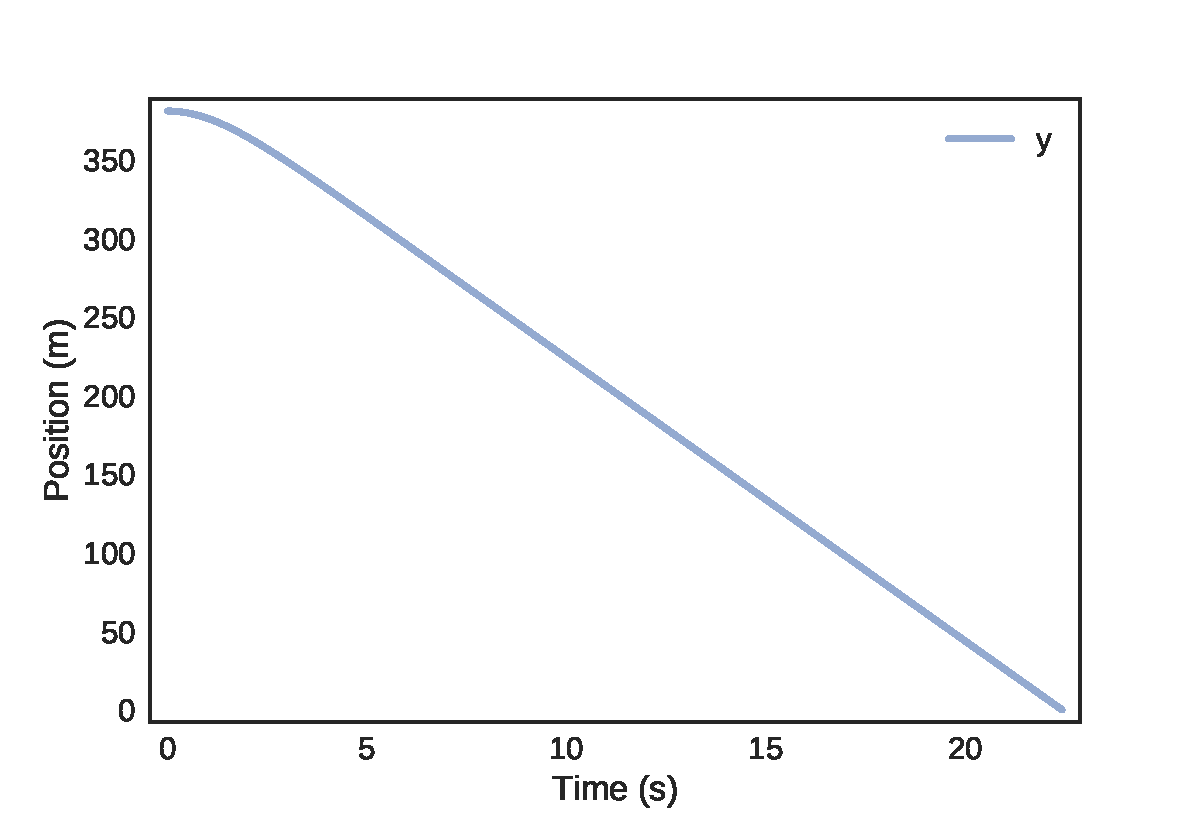
\includegraphics[height=3in]{figs/chap09-fig02.pdf}}
\caption{Height of the penny versus time, with air resistance.}
\label{chap09-fig02}
\end{figure}

Figure~\ref{chap09-fig02} shows the result.  It only takes a few seconds for the penny to accelerate up to terminal velocity; after that, velocity is constant, so height as a function of time is a straight line.
\index{terminal velocity}


\section{Dropping quarters}

In the previous sections, we were given an estimate of terminal velocity, based on measurements, and we used it to estimate the drag coefficient, $C_d$.  Now suppose that we are given flight time, instead.  Can we use that to estimate $C_d$ and terminal velocity?
\index{quarter}

Suppose I drop a quarter off the Empire State Building and find that it takes \SI{19.1}{\second} to reach the sidewalk.  Here's a \py{Condition} object with the parameters of a quarter (from \url{http://modsimpy.com/quarter}) and the measured duration:
\index{Condition object}

\begin{python}
condition = Condition(height = 381 * m,
                      v_init = 0 * m / s,
                      g = 9.8 * m/s**2,
                      mass = 5.67e-3 * kg,
                      diameter = 24.26e-3 * m,
                      rho = 1.2 * kg/m**3,
                      duration = 19.1 * s)
\end{python}

And here's a revised version of \py{make_system}:
\index{\py{make_system}}
\index{unpack}

\begin{python}
def make_system(condition):
    unpack(condition)
    
    init = State(y=height, v=v_init)
    area = np.pi * (diameter/2)**2
    ts = linspace(0, duration, 101)
    
    return System(init=init, g=g, mass=mass, rho=rho,
                  C_d=C_d, area=area, ts=ts)
\end{python}

This version does not expect the \py{Condition} object to contain \py{v_term}, but it does expect \py{C_d}.  We don't know what \py{C_d} is,  so we'll start with an initial guess and go from there:

\begin{python}
condition.set(C_d=0.4)
system = make_system(condition)
run_odeint(system, slope_func)
\end{python}

\py{Condition} objects provide a function called \py{set} that we can use to modify the condition variables.  With \py{C_d=0.4}, the height of the quarter after \SI{19.1}{\second} is \SI{-11}{\meter}.  That means the quarter is moving a bit too fast, which means our estimate for the drag coefficient is too low.  We could improve the estimate by trial and error, or we could get \py{fsolve} to do it for us.  
\index{fsolve}
\index{error function}
\index{function!error}

To use \py{fsolve}, we need an error function, which we can define by encapsulating the previous lines of code:

\begin{python}
def height_func(C_d, condition):
    condition.set(C_d=C_d)
    system = make_system(condition)
    run_odeint(system, slope_func)
    y, v = final_state(system.results)
    return y
\end{python}

\py{height_func} takes a hypothetical value of \py{C_d} as a parameter.  It runs the simulation with the given value of \py{C_d} and returns the final height after \SI{19.1}{\second}.

When we get the value of \py{C_d} right, the result should be 0, so we can use \py{fsolve} to find it:

\begin{python}
fsolve(height_func, 0.4, condition)
\end{python}

As we saw in Section~\ref{fsolve}, \py{fsolve} takes the error function and the initial guess as parameters.  Any additional parameters we give to \py{fsolve} are passed along to \py{height_func}.  In this case, we provide \py{condition} as an argument to \py{fsolve} so we can use it inside \py{height_func}.

The result from \py{fsolve} is 0.43, which is very close to the drag coefficient we computed for the penny, 0.44.  Although it is plausible that different coins would have similar drag coefficients, we should not take this result too seriously.  Remember that I chose the terminal velocity of the penny arbitrarily from the estimated range.  And I completely fabricated the flight time for the quarter.

Nevertheless, the methods we developed for estimating \py{C_d}, based on terminal velocity or flight time, are valid, subject to the precision of the measurements.

These methods demonstrate two ways to use models to solve problems, sometimes called {\bf forward} and {\bf inverse} problems.  In a forward problem, you are given the parameters of the system and asked to predict how it will behave.  In an inverse problem, you are given the behavior of the system and asked to infer the parameters.  See \url{http://modsimpy.com/inverse}. 
\index{forward problem}
\index{inverse problem}
\index{parameter of a system}


\chapter{Two dimensions}

In the previous chapter we modeled objects moving in one dimension, with and without drag.  Now let's move on to two dimensions, and baseball!

You can view the code for this chapter at \url{http://modsimpy.com/chap10}.  For instructions for downloading and running the code, see Section~\ref{code}.


\section{The Manny Ramirez problem}
\label{manny}

Manny Ramirez is a former member of the Boston Red Sox (an American baseball team) who was notorious for a relaxed attitude and a taste for practical jokes that his managers did not always appreciate.  Our objective in this chapter is to solve the following Manny-inspired problem:
\index{Ramirez, Manny}
\index{Fenway Park}
\index{baseball}

{\it What is the minimum effort required to hit a home run in Fenway Park?}

Fenway Park is a baseball stadium in Boston, Massachusetts.  One of its most famous features is the ``Green Monster", which is a wall in left field that is unusually close to home plate, only 310 feet.  To compensate for the short distance, the wall is unusually high, at 37 feet (see \url{http://modsimpy.com/wally}).
\index{Green Monster}

We want to find the minimum velocity at which a ball can leave home plate and still go over the Green Monster.  We'll proceed in the following steps:
\index{velocity}

\begin{enumerate}

\item We'll model the flight of a baseball through air.

\item For a given velocity, we'll find the optimal {\bf launch angle}, that is, the angle the ball should leave home plate to maximize its height when it reaches the wall.
\index{launch angle}

\item Then we'll find the minimal velocity that clears the wall, given that it has the optimal launch angle.

\end{enumerate}

As usual, we'll have to make some modeling decisions.  To get started, we'll ignore any spin that might be on the ball, and the resulting Magnus force (see \url{http://modsimpy.com/magnus}).
\index{Magnus force}

As a result, we'll assume that the ball travels in the plane above the left field line, so we'll run simulations in two dimensions, rather than three.

But we will take into account air resistance.  Based on what we learned about falling coins, it seems likely that air resistance has a substantial effect on the flight of a baseball.
\index{air resistance}

To model air resistance, we'll need the mass, frontal area, and drag coefficient of a baseball.  Mass and diameter are easy to find (see \url{http://modsimpy.com/baseball}).  Drag coefficient is only a little harder; according to a one-pager from NASA\footnote{``Drag on a Baseball", available from \url{http://modsimpy.com/nasa}}, the drag coefficient of a baseball is approximately 0.3.
\index{drag coefficient}
\index{NASA}

However, this value {\em does} depend on velocity\footnote{Adair, {\it The Physics of Baseball}, Third Edition, Perennial, 2002}.  At low velocities it might be as high as 0.5, and at high velocities as low as 0.29.  Furthermore, the transition between these regimes typically happens exactly in the range of velocities we are interested in, around \SI{40}{\meter\per\second}.

To get started, I'll assume that the drag coefficient does not depend on velocity, but this is an issue we might want to revisit.


\section{Vectors}

Now that we are working in two dimensions, we will find it useful to work with {\bf vector quantities}, that is, quantities that represent both a magnitude and a direction.  We will use vectors to represent positions, velocities, accelerations, and forces in two and three dimensions. 
\index{Vector object}
\index{array}
\index{NumPy}

The \py{modsim} library provides a \py{Vector} object that represents a vector quantity.  A \py{Vector} object is a like a NumPy array; it contains elements that represent the {\bf components} of the vector.  For example, in a \py{Vector} that represents a position in space, the components are the $x$ and $y$ coordinates (and a $z$ coordinate in 3-D).  A \py{Vector} object also has units, like the quantities we've seen in previous chapters.  
\index{unit}

You can create a \py{Vector} by specifying its components.  The following \py{Vector} represents a point \SI{3}{\meter} to the right (or east) and \SI{4}{\meter} up (or north) from an implicit origin:
\index{component}

\begin{python}
A = Vector(3, 4) * m
\end{python}

You can access the components of a \py{Vector} by name, using the dot operator; for example, \py{A.x} or \py{A.y}.  You can also access them by index, using brackets, like \py{A[0]} or \py{A[1]}.

Similarly, you can get the magnitude and angle using the dot operator, \py{A.mag} and \py{A.angle}.  {\bf Magnitude} is the length of the vector: if the \py{Vector} represents position, magnitude is the distance from the origin; if it represents velocity, magnitude is speed, that is, how fast the object is moving, regardless of direction.
\index{angle}
\index{magnitude}

The {\bf angle} of a \py{Vector} is its direction, expressed as the angle in radians from the positive x-axis.  In the Cartesian plane, the angle \SI{0}{\radian} is due east, and the angle \SI{\pi}{\radian} is due west. 
\index{radian}

\py{Vector} objects support most mathematical operations, including addition and subtraction:

\begin{python}
B = Vector(1, 2) * m
A + B
A - B
\end{python}

For the definition and graphical interpretation of these operations, see \url{http://modsimpy.com/vecops}.
\index{vector operation}

When you add and subtract \py{Vector} objects, the \py{modsim} library uses NumPy and Pint to check that the operands have the same number of dimensions and units.  The notebook for this chapter shows examples for working with \py{Vector} objects.
\index{dimensions}

One note on working with angles: in mathematics, we almost always represent angle in radians, and most Python functions expect angles in radians.  But people often think more naturally in degrees.  It can be awkward, and error-prone, to use both units in the same program.  Fortunately, Pint makes it possible to represent angles using quantities with units.
\index{degree}

As an example, I'll get the \py{degree} unit from \py{UNITS}, and create a quantity that represents 45 degrees:

\begin{python}
degree = UNITS.degree
angle = 45 * degree
\end{python}

Then if we need to convert to radians we can use the \py{to} function
\index{\py{to}}

\begin{python}
radian = UNITS.radian
rads = angle.to(radian)
\end{python}

Alternatively, if we know that a quantity is represented in degrees, we can use \py{np.deg2rad} to convert to radians.  However, unlike the \py{to} function, \py{np.deg2rad} does no error checking!
\index{deg2rad}

If you are given an angle and velocity, you can make a \py{Vector} by converting to Cartesian coordinates using \py{pol2cart}.  To demonstrate, I'll extract the angle and magnitude of \py{A}:
\index{pol2cart}

\begin{python}
mag = A.mag
angle = A.angle
\end{python}

And then make a new \py{Vector} with the same components:

\begin{python}
x, y = pol2cart(angle, mag)
Vector(x, y)
\end{python}



\section{Modeling baseball flight}

Now we're ready to simulate the flight of the baseball.  As in Section~\ref{condition}, I'll create a \py{Condition} object that contains the parameters of the system:
\index{Condition object}

\begin{python}
condition = Condition(x = 0 * m, 
                      y = 1 * m,
                      g = 9.8 * m/s**2,
                      mass = 145e-3 * kg,
                      diameter = 73e-3 * m,
                      rho = 1.2 * kg/m**3,
                      C_d = 0.3,
                      angle = 45 * degree,
                      velocity = 40 * m / s,
                      duration = 5.1 * s)
\end{python}

Using the center of home plate as the origin, the initial height is about \SI{1}{\meter}.  The initial velocity is \SI{40}{\meter\per\second} at a launch angle of \SI{45}{\degree}.  The mass, diameter, and drag coefficient of the baseball are from the sources in Section~\ref{manny}.  The acceleration of gravity, \py{g}, is a well-known quantity, and the density of air, \py{rho}, is based on a temperature of \SI{20}{\celsius} at sea level (see \url{http://modsimpy.com/tempress}).
 I chose the value of \py{duration} to run the simulation long enough for the ball to land on the ground.
\index{density}

The following function uses the \py{Condition} object to make a \py{System} object.  Again, this two-step process reduces the number of variables in the \py{System} object, and makes it easier to work with functions like \py{fsolve}.
\index{System object}
\index{\py{make_system}}

\begin{python}
def make_system(condition):
    unpack(condition)
	
    theta = np.deg2rad(angle)
    vx, vy = pol2cart(theta, velocity)
    init = State(x=x, y=y, vx=vx, vy=vy)
    area = np.pi * (diameter/2)**2
    ts = linspace(0, duration, 101)
    
    return System(init=init, g=g, mass=mass, 
                  area=area, rho=rho, C_d=C_d, ts=ts)
\end{python}

After unpacking \py{Condition}, we can access the variables it contains without using the dot operator.
\index{dot operator}
\index{operator!dot}
\index{unpack}

\py{make_system} uses \py{np.deg2rad} to convert \py{angle} to radians and \py{pol2cart} to compute the $x$ and $y$ components of the initial velocity.  Then it makes the initial \py{State} object, computes \py{area} and \py{ts}, and creates the \py{System} object.
\index{deg2rad}
\index{State object}
\index{slope function}
\index{function!slope}

Now we're ready for a slope function:

\begin{python}
def slope_func(state, t, system):
    x, y, vx, vy = state
    unpack(system)
    
    a_grav = Vector(0, -g)

    v = Vector(vx, vy)
    f_drag = -rho * v.mag * v * C_d * area / 2
    a_drag = f_drag / mass
    
    a = a_grav + a_drag
    
    return v.x, v.y, a.x, a.y
\end{python}

As usual, the parameters of the slope function are a \py{State} object, time, and a \py{System} object.  In this example, we don't use \py{t}, but we can't leave it out because when \py{odeint} calls the slope function, it always provides the same arguments, whether they are needed or not.

The \py{State} object has four variables: \py{x} and \py{y} are the components of position; \py{vx} and \py{vy} are the components of velocity.
\index{state variable}

The return values from the slope function are the derivatives of these components.  The derivative of position is velocity, so the first two return values are just \py{vx} and \py{vy}, the values we extracted from the \py{State} object.  The derivative of velocity is acceleration, and that's what we have to compute.

The total acceleration of the baseball is the sum of accelerations due to gravity and drag.  These quantities have both magnitude and direction, so we'll use \py{Vector} objects to represent them.  Here's how it works:

\begin{itemize}

\item \py{a_grav} is the \py{Vector} representation of acceleration due to gravity, with magnitude \py{g} and direction along the negative y-axis.
\index{acceleration}

\item \py{v} is the \py{Vector} representation of velocity, which we create using the components \py{vx} and \py{vy}.  This representation makes it easier to compute the drag force, which I explain in more detail below.
\index{velocity}

\item \py{f_drag} is drag force, which is also a \py{Vector} quantity, with units of \si{\kilogram\meter\per\second\squared}, also known as newtons (\si{\newton}).
\index{drag force}

\item \py{a_drag} is acceleration due to drag, which we get by dividing \py{f_drag} by mass.  The result is in units of acceleration, \si{\meter\per\second\squared}.

\item \py{a} is total acceleration due to all forces, from which we can extract the components \py{a.x} and \py{a.y}.

\end{itemize}

The last thing I have to explain is the vector form of the drag equation.  In Section~\ref{drag} we saw the scalar form (a {\bf scalar} is a single value, as contrasted with a vector, which contains components):
\index{drag equation}
\index{scalar}

\[ F_d = \frac{1}{2}~\rho~v^2~C_d~A \]

This form was sufficient when \py{v} represented the magnitude of velocity and all we wanted was the magnitude of drag force.  But now \py{v} is a \py{Vector} and we want both the magnitude and angle of drag.
\index{magnitude}
\index{angle}

We can do that by replacing $v^2$, in the equation, with a vector that has the opposite direction as \py{v} and magnitude \py{v.mag**2}.  In math notation, we can write

\[ \vec{F}_d = -\frac{1}{2}~\rho~|v|~\vec{v}~C_d~A \]

Where $|v|$ indicates the magnitude of $v$ and the arrows on $\vec{F}_d$ and $\vec{v}$ indicate that they are vectors.  Negation reverses the direction of a vector, so $\vec{F}_d$ is in the opposite direction of $\vec{v}$.

Translating to Python we have:

\begin{python}
f_drag = -rho * v.mag * v * C_d * area / 2
\end{python}

Using vectors to represent forces and accelerations makes the code concise, readable, and less error-prone.  In particular, when we add \py{a_grav} and \py{a_drag}, the directions are likely to be correct, because they are encoded in the \py{Vector} objects.  And the units are certain to be correct, because otherwise Pint would report an error.
\index{Pint}

As always, we can test the slope function by running it with the initial conditions:

\begin{python}
slope_func(system.init, 0, system)
\end{python}


\section{Trajectories}

Now we're ready to run the simulation:
\index{\py{run_odeint}}

\begin{python}
run_odeint(system, slope_func)
\end{python}

The result is a \py{TimeFrame} object with one column for each of the state variables, \py{x}, \py{y}, \py{vx}, and \py{vy}.  We can extract the $x$ and $y$ components like this:
\index{TimeFrame object}

\begin{python}
xs = system.results.x
ys = system.results.y
\end{python}

And plot them like this:

\begin{python}
plot(xs, label='x')
plot(ys, label='y')
\end{python}

\begin{figure}
\centerline{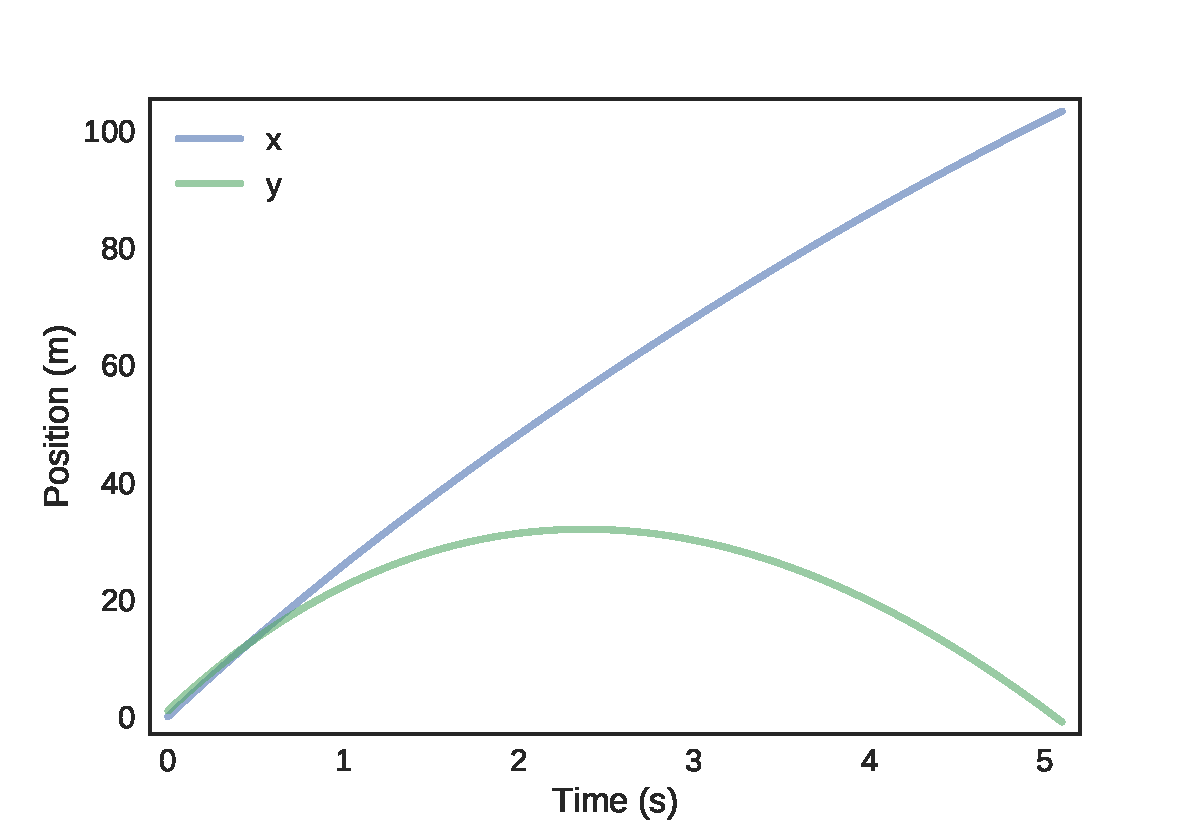
\includegraphics[height=3in]{figs/chap10-fig01.pdf}}
\caption{Simulated baseball flight, $x$ and $y$ components of position as a function of time.}
\label{chap10-fig01}
\end{figure}

Figure~\ref{chap10-fig01} shows the result.  As expected, the $x$ component increases monotonically, with decreasing velocity.  And the $y$ position climbs initially and then descends, falling slightly below \SI{0}{\meter} after \SI{5.1}{\second}.
\index{monotonic}

Another way to view the same data is to plot the $x$ component on the x-axis and the $y$ component on the y-axis, so the plotted line follows the trajectory of the ball through the plane:

\begin{python}
plot(xs, ys, label='trajectory')
\end{python}

\begin{figure}
\centerline{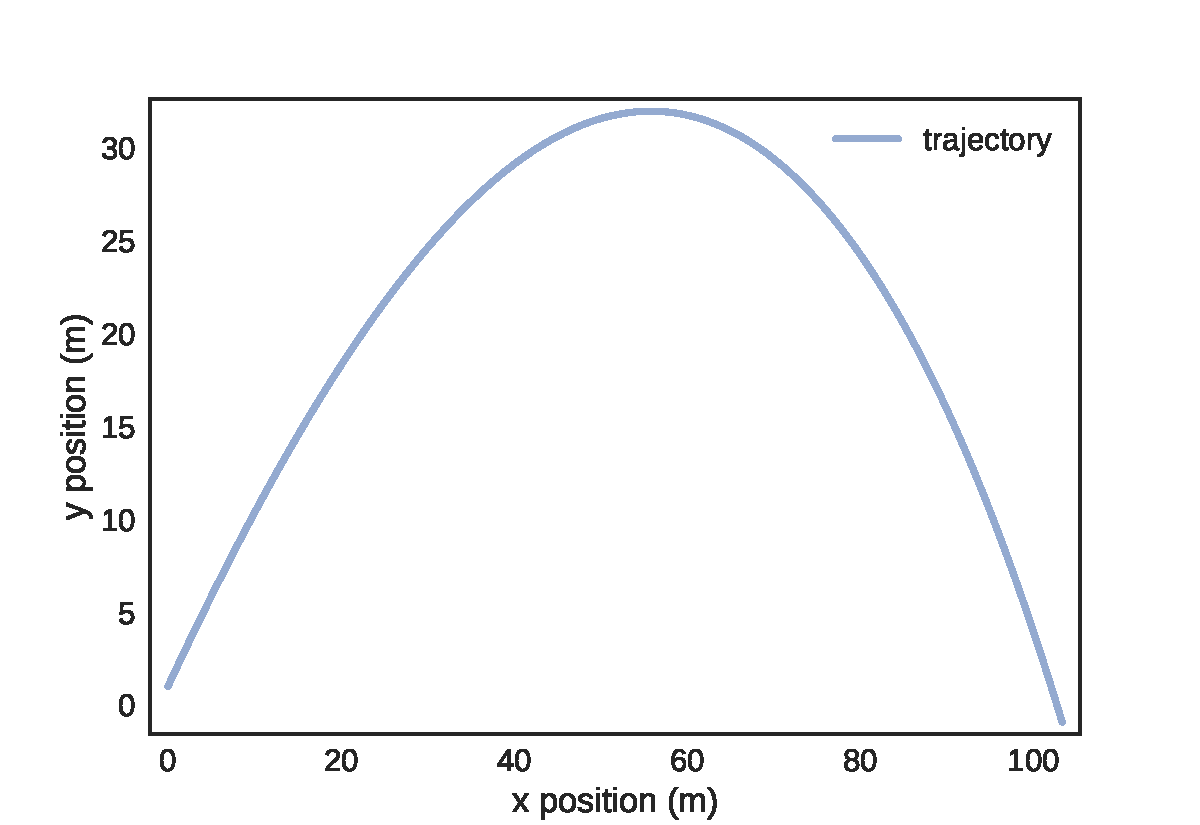
\includegraphics[height=3in]{figs/chap10-fig02.pdf}}
\caption{Simulated baseball flight, trajectory plot.}
\label{chap10-fig02}
\end{figure}

Figure~\ref{chap10-fig02} shows this way of visualizing the results, which is called a {\bf trajectory plot} (see \url{http://modsimpy.com/trajec}).
\index{trajectory plot}

A trajectory plot can be easier to interpret than a time series plot, because it shows what the motion of the projectile would look like (at least from one point of view).  Both plots can be useful, but don't get them mixed up!  If you are looking at a time series plot and interpreting it as a trajectory, you will be very confused.

Another useful way to visualize the results is animation.  You can create animations using the \py{plot} function from the \py{modsim} library, with the \py{update} argument, which tells \py{plot} that the coordinates you provide should update the old coordinates.  Here's an example:
\index{animation}
\index{plot}

\begin{python}
for x, y in zip(xs, ys):
    plot(x, y, 'bo', update=True)
    sleep(0.01)
\end{python}

This example uses two features we have not seen before:

\begin{itemize}

\item \py{zip} takes two sequences (in this case they are \py{Series} objects) and ``zips" them together; that is, it loops through both of them at the same time, selecting corresponding elements from each.  So each time through the loop, \py{x} and \py{y} get the next elements from \py{xs} and \py{ys}.
\index{zip}

\item \py{sleep} causes the program to pause for a given duration, in seconds.
\index{sleep}

\end{itemize}

You can see what the results look like in the notebook for this chapter.


\section{Finding the range}

Suppose we want to find the launch angle that maximizes {\bf range}, that is, the distance the ball travels in the air before landing.  Assuming that the simulation runs long enough for the ball to land, we can compute the range like this:
\index{range}

\begin{enumerate}

\item Find the time when the height of the ball is maximized and select the part of the trajectory where the ball is falling.  We have to do this in order to avoid problems with interpolation (see Section~\ref{sidewalk}).

\item Then we use \py{interpolate} to find the time when the ball hits the ground, \py{t_land}.

\item Finally, we compute the $x$ component at \py{t_land}.

\end{enumerate}

Here's the function that does all that:

\begin{python}
def interpolate_range(results):
    xs = results.x
    ys = results.y

    t_peak = ys.idxmax()
    
    descent = ys.loc[t_peak:]
    T = interp_inverse(descent)
    t_land = T(0)
    
    X = interpolate(xs, kind='cubic')
    return X(t_land)
\end{python}

\py{interpolate_range} uses \py{idxmax} to find the time when the ball hits its peak (see Section~\ref{metrics}).
\index{idxmax}

Then it uses \py{ys.loc} to extract only the points from \py{t_peak} to the end.  The index in brackets includes a colon (\py{:}), which indicates that it is a {\bf slice index}.  In general, a slice selects a range of elements from a \py{Series}, specifying the start and end indices.  For example, the following slice selects elements from \py{t_peak} to \py{t_land}, including both:
\index{loc}
\index{slice index}

\begin{python}
ys.loc[t_peak:t_land]
\end{python}

If we omit the first index, like this:

\begin{python}
ys.loc[:t_land]
\end{python}

we get everything from the beginning to \py{t_land}.  If we omit the second index, as in \py{interpolate_range}, we get everything from \py{t_peak} to the end of the \py{Series}.  For more about indexing with \py{loc}, see \url{http://modsimpy.com/loc}.

Next it uses \py{interp_inverse}, which we saw in Section~\ref{sidewalk}, to make \py{T}, which is an interpolation function that maps from height to time.  So \py{t_land} is the time when height is 0.
\index{interpolate}
\index{\py{interp_inverse}}

Finally, it uses \py{interpolate} to make \py{X}, which is an interpolation function that maps from time to $x$ component.  So \py{X(t_land)} is the distance from home plate when the ball lands.

We can call \py{interpolate_range} like this:

\begin{python}
interpolate_range(system.results)
\end{python}

The result is \SI{103}{\meter}, which is about 337 feet.


\section{Optimization}

To find the angle that optimizes range, we need a function that takes launch angle as a parameter and returns range:
\index{optimization}

\begin{python}
def range_func(angle, condition):    
    condition.set(angle=angle)
    system = make_system(condition)
    run_odeint(system, slope_func)
    x_range = interpolate_range(system.results)
    return x_range
\end{python}

We can call \py{range_func} directly like this:

\begin{python}
range_func(45, condition)
\end{python}

And we can sweep a sequence of angles like this:
\index{parameter sweep}
\index{SweepSeries object}

\begin{python}
angles = linspace(30, 60, 11)
sweep = SweepSeries()

for angle in angles:
    x_range = range_func(angle, condition)
    print(angle, x_range)
    sweep[angle] = x_range
\end{python}

\begin{figure}
\centerline{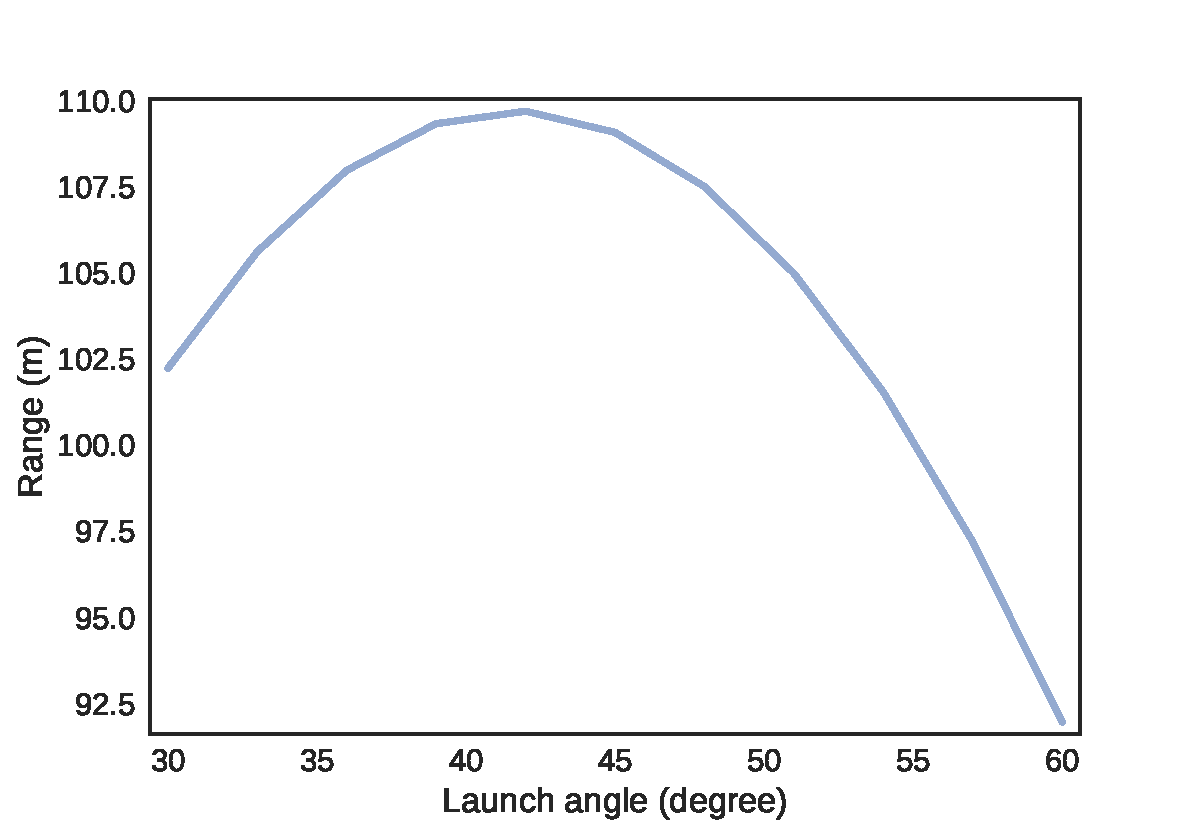
\includegraphics[height=3in]{figs/chap10-fig03.pdf}}
\caption{Distance from home plate as a function of launch angle, with fixed velocity.}
\label{chap10-fig03}
\end{figure}

Figure~\ref{chap10-fig03} shows the results.  It looks like the optimal angle is between \SI{40}{\degree} and \SI{45}{\degree} (at least for this definition of ``optimal").

We can find the optimal angle more precisely and more efficiently using \py{max_bounded}, which is a function in the \py{modsim} library that uses \py{scipy.opimize.minimize_scalar} (see \url{http://modsimpy.com/minimize}).
\index{scalar}
\index{\py{max_bounded}}
\index{SciPy}
\index{\py{minimize_scalar}}

Here's how we run it:

\begin{python}
res = max_bounded(range_func, [0, 90], condition)
\end{python}

The first parameter is the function we want to maximize.  The second is the range of values we want to search; in this case it's the range of angles from \SI{0}{\degree} to \SI{90}{\degree}.  The third argument is the \py{Condition} object, which gets passed along as an argument when \py{max_bounded} calls \py{range_func}.
\index{Condition object}

The result from \py{max_bounded} is an \py{OptimizeResult} object, which contains several variables.  The ones we want are \py{x}, which is the angle that yielded the highest range, and \py{fun}, which is the value of \py{range_func} when it's evaluated at \py{x}, that is, range when the baseball is launched at the optimal angle.
\index{OptimizeResult object}


\section{Finishing off the problem}

In the notebook for this chapter, you'll have to chance to finish off the Manny Ramirez problem.  There are a few things you'll have to do:

\begin{itemize}

\item In the previous section the ``optimal" launch angle is the one that maximizes range, but that's not what we want.  Rather, we want the angle that maximizes the height of the ball when it gets to the wall (310 feet from home plate).  So you'll have to write a height function to compute it, and then use \py{max_bounded} to find the revised optimum.

\item Once you can find the optimal angle for any velocity, you have to find the minimum velocity that gets the ball over the wall.  You'll write a function that takes a velocity as a parameter, computes the optimal angle for that velocity, and returns the height of the ball, at the wall, using the optimal angle.

\item Finally, you'll use \py{fsolve} to find the velocity that makes the height, at the wall, just barely 37 feet.  
\index{fsolve}

\end{itemize}

The notebook provides some additional hints, but at this point you should have everything you need.  Good luck!

If you enjoy this exercise, you might be interested in this paper: ``How to hit home runs: Optimum baseball bat swing parameters for maximum range trajectories", by Sawicki, Hubbard, and Stronge, at \url{http://aapt.scitation.org/doi/abs/10.1119/1.1604384}.


\chapter{Rotation}

In this chapter we model systems that involve rotating objects.  In general, rotation is complicated:  in three dimensions, objects can rotate around three axes; objects are often easier to spin around some axes than others; and they may be stable when spinning around some axes but not others.  
\index{rotation}

If the configuration of an object changes over time, it might become easier or harder to spin, which explains the surprising dynamics of gymnasts, divers, ice skaters, etc.

And when you apply a twisting force to a rotating object, the effect is often contrary to intuition.  For an example, see this video on gyroscopic precession \url{http://modsimpy.com/precess}.
\index{gyroscopic precession}

In this chapter, we will not take on the physics of rotation in all its glory.  Rather, we will focus on simple scenarios where all rotation and all twisting forces are around a single axis.  In that case, we can treat some vector quantities as if they were scalars (in the same way that we sometimes treat velocity as a scalar with an implicit direction).
\index{scalar}

This approach makes it possible to simulate and analyze many interesting systems, but you will also encounter systems that would be better approached with the more general toolkit.

The fundamental ideas in this chapter are {\bf angular velocity}, {\bf angular acceleration}, {\bf torque}, and {\bf moment of inertia}.  If you are not already familiar with these concepts, I will define them as we go along, and I will point to additional reading.

As an exercise at the end of the chapter, you will use these tools to simulate the behavior of a yo-yo (see \url{http://modsimpy.com/yoyo}).  But we'll work our way up to it gradually, starting with toilet paper.

You can view the code for this chapter at \url{http://modsimpy.com/chap11}.  For instructions for downloading and running the code, see Section~\ref{code}.


\section{The physics of toilet paper}
\label{paper}

As a simple example of a system with rotation, we'll simulate the manufacture of a roll of toilet paper.  Starting with a cardboard tube at the center, we will roll up \SI{47}{\meter} of paper, the typical length of a roll of toilet paper in the U.S. (see \url{http://modsimpy.com/paper}).
\index{toilet paper}

\begin{figure}
\centerline{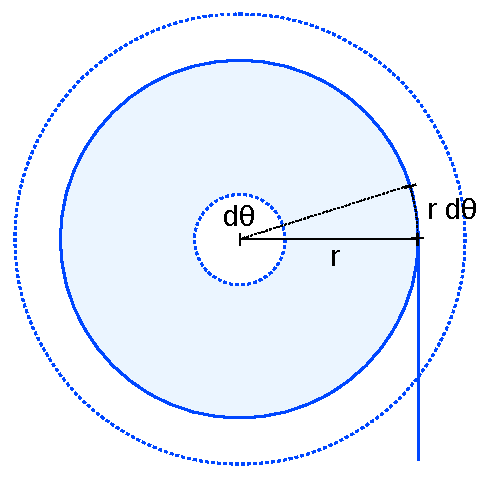
\includegraphics[height=2.5in]{figs/paper_roll.pdf}}
\caption{Diagram of a roll of toilet paper, showing change in paper length as a result of a small rotation, $d\theta$.}
\label{paper_roll}
\end{figure}

Figure~\ref{paper_roll} shows a diagram of the system: $r$ represents the radius of the roll at a point in time.  Initially, $r$ is the radius of the cardboard core, $R_{min}$.  When the roll is complete, $r$ is $R_{max}$.

I'll use $\theta$ to represent the total rotation of the roll in radians.  In the diagram, $d\theta$ represents a small increase in $\theta$, which corresponds to a distance along the circumference of the roll of $r~d\theta$.
\index{radian}

Finally, I'll use $y$ to represent the total length of paper that's been rolled.  Initially, $\theta=0$ and $y=0$.  For each small increase in $\theta$, there is a corresponding increase in $y$:
%
\[ dy = r~d\theta \]
%
If we divide both sides by a small increase in time, $dt$, we get a differential equation for $y$ as a function of time.
%
\[ \frac{dy}{dt} = r \frac{d\theta}{dt} \]
%
As we roll up the paper, $r$ increases, too.  Assuming that $r$ increases by a fixed amount per revolution, we can write
%
\[ dr = k~d\theta \]
%
Where $k$ is an unknown constant we'll have to figure out.  Again, we can divide both sides by $dt$ to get a differential equation in time:
%
\[ \frac{dr}{dt} = k \frac{d\theta}{dt} \]
%
Finally, let's assume that $\theta$ increases at a constant rate of \SI{10}{\radian\per\second} (about 95 revolutions per minute):
%
\[ \frac{d\theta}{dt} = 10  \]
%
This rate of change is called an {\bf angular velocity}.  Now we have a system of three differential equations we can use to simulate the system.
\index{angular velocity}
\index{differential equation}

\section{Implementation}
\label{papersim}

At this point we have a pretty standard process for writing simulations like this.  First, we'll get the units we need from Pint:
\index{Pint}

\begin{python}
radian = UNITS.radian
m = UNITS.meter
s = UNITS.second
\end{python}

And create a \py{Condition} object with the parameters of the system:
\index{Condition object}

\begin{python}
condition = Condition(Rmin = 0.02 * m,
                      Rmax = 0.055 * m,
                      L = 47 * m,
                      duration = 130 * s)
\end{python}

\py{Rmin} and \py{Rmax} are the initial and final values for the radius, \py{r}.  \py{L} is the total length of the paper, and \py{duration} is the length of the simulation in time.

Then we use the \py{Condition} object to make a \py{System} object:
\index{System object}
\index{\py{make_system}}

\begin{python}
def make_system(condition):
    unpack(condition)
    
    init = State(theta = 0 * radian,
                 y = 0 * m,
                 r = Rmin)
    
    k = estimate_k(condition)
    ts = linspace(0, duration, 101)
    
    return System(init=init, k=k, ts=ts)
\end{python}

The initial state contains three variables, \py{theta}, \py{y}, and \py{r}.
\index{unpack}

To get started, we'll estimate a reasonable value for \py{k}; then in Section~\ref{paper_analysis} we'll figure it out exactly.  Here's how we compute the estimate:

\begin{python}
def estimate_k(condition):
    unpack(condition)
    
    Ravg = (Rmax + Rmin) / 2
    Cavg = 2 * pi * Ravg
    revs = L / Cavg
    rads = 2 * pi * revs
    k = (Rmax - Rmin) / rads
    return k
\end{python}

\py{Ravg} is the average radius, half way between \py{Rmin} and \py{Rmax}, so \py{Cavg} is the circumference of the roll when \py{r} is \py{Ravg}.

\py{revs} is the total number of revolutions it would take to roll up length \py{L} if \py{r} were constant at \py{Ravg}.  And \py{rads} is just \py{revs} converted to radians.

Finally, \py{k} is the change in \py{r} for each radian of revolution.  For these parameters, \py{k} is about \py{2.8e-5} \si{\meter\per\radian}.

Now we can use the differential equations from Section~\ref{paper} to write a slope function:
\index{slope function}
\index{Function!slope}

\begin{python}
def slope_func(state, t, system):
    theta, y, r = state
    unpack(system)
    
    omega = 10 * radian / s
    dydt = r * omega
    drdt = k * omega
    
    return omega, dydt, drdt
\end{python}

As usual, the slope function takes a \py{State} object, a time, and a \py{System} object.  The \py{State} object contains the hypothetical values of \py{theta}, \py{y}, and \py{r} at time \py{t}.  The job of the slope function is to compute the time derivatives of these values.  The time derivative of \py{theta} is angular velocity, which is often denoted \py{omega}.
\index{State object}

Now we can run the simulation like this:

\begin{python}
run_odeint(system, slope_func)
\end{python}

\begin{figure}
\centerline{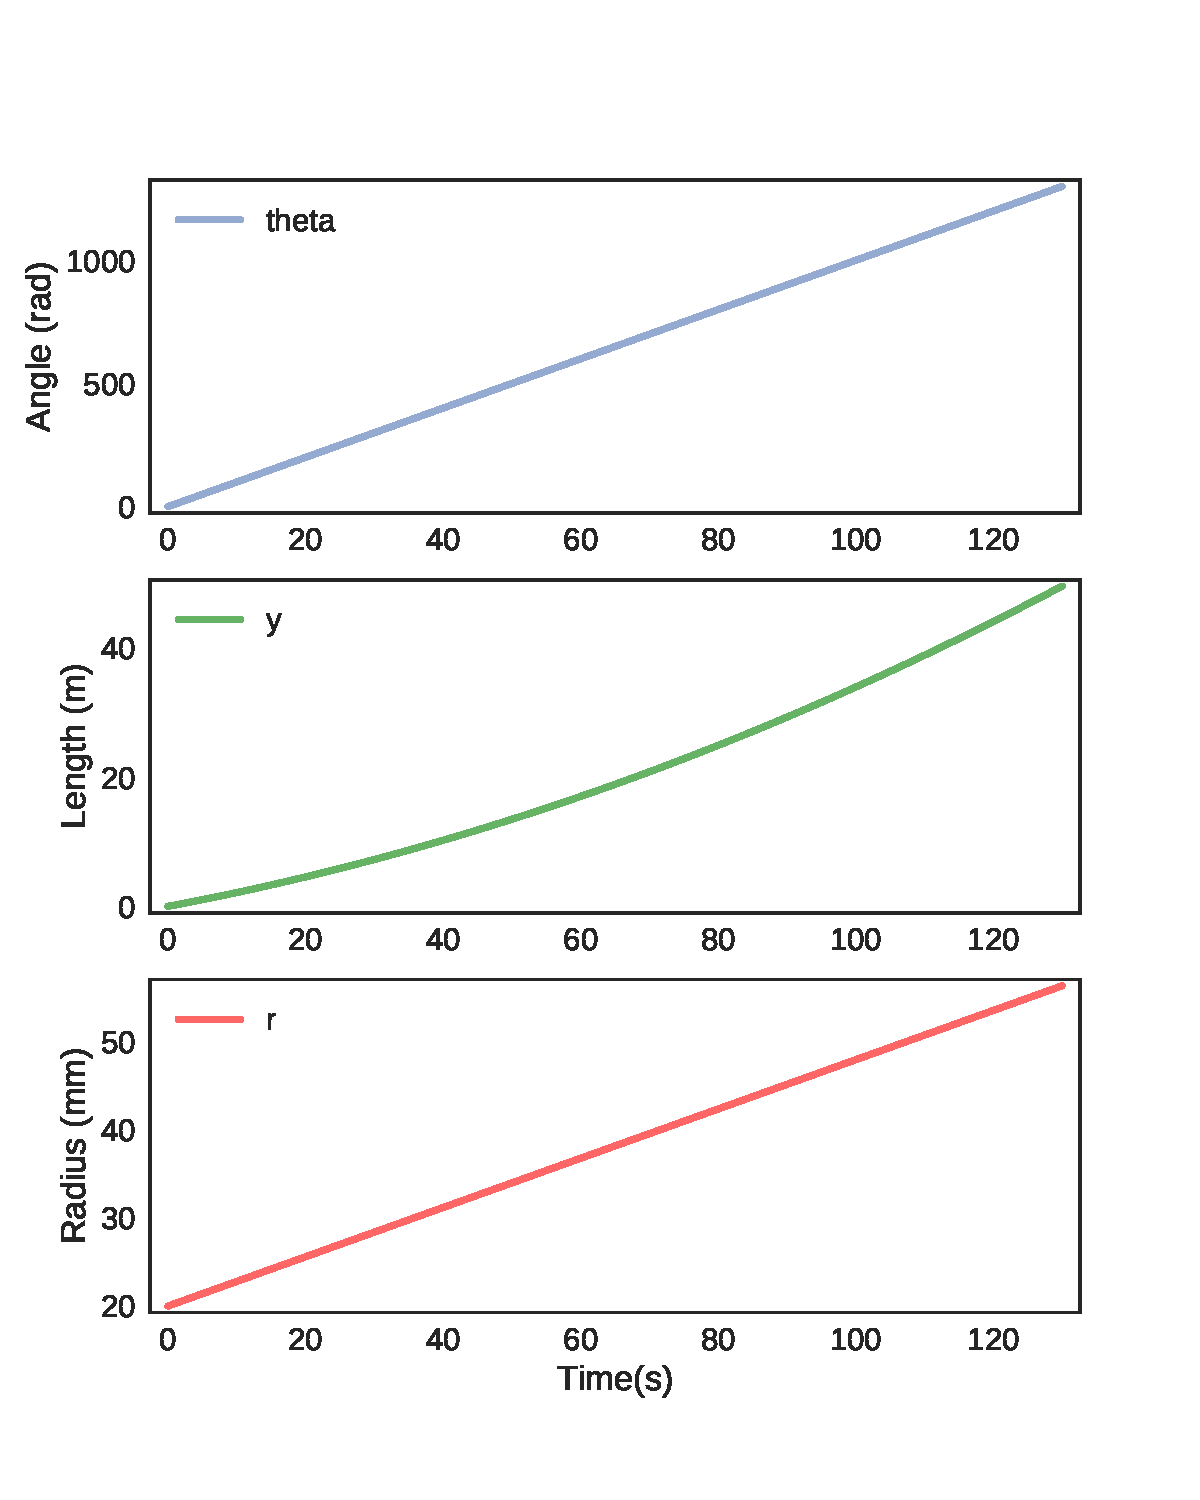
\includegraphics[width=3in]{figs/chap11-fig01.pdf}}
\caption{Results from paper rolling simulation, showing rotation, length, and radius over time.}
\label{chap11-fig01}
\end{figure}

Figure~\ref{chap11-fig01} shows the results.  \py{theta} grows linearly over time, as we should expect.  As a result, \py{r} also grows linearly.  But since the derivative of \py{y} depends on \py{r}, and \py{r} is increasing, \py{y} grows with increasing slope.

Because this system is so simple, it is almost silly to simulate it.  As we'll see in the next section, it is easy enough to solve the differential equations analytically.  But it is often useful to start with a simple simulation as a way of exploring and checking assumptions.

In order to get the simulation working, we have to get the units right, which can help catch conceptual errors early.  And by plugging in realistic parameters, we can detect errors that cause unrealistic results.  For example, in this system we can check:

\begin{itemize}

\item The total time for the simulation is about 2 minutes, which seems plausible for the time it would take to roll \SI{47}{\meter} of paper.

\item The final value of \py{theta} is about \SI{1250}{\radian}, which corresponds to about 200 revolutions, which also seems plausible.

\item The initial and final values for \py{r} are consistent with \py{Rmin} and \py{Rmax}, as we intended when we chose \py{k}.

\end{itemize}

But now that we have a working simulation, it is also useful to do some analysis.


\section{Analysis}
\label{paper_analysis}

The differential equations in Section~\ref{paper} are simple enough that we can just solve them.  Since angular velocity is constant:
%
\[ \frac{d\theta}{dt} = \omega  \]
%
We can find $\theta$ as a function of time by integrating both sides:
%
\[ \theta(t) = \omega t + C_1 \]
%
With the initial condition $\theta(0)=0$,  we find $C_1=0$.  Similarly,
%
\begin{equation}
\frac{dr}{dt} = k \omega                    \label{eqn1}
\end{equation}
%
So
%
\[ r(t) = k \omega t + C_2 \]
%
With the initial condition $r(0)=R_{min}$,  we find $C_2=R_{min}$.  Then we can plug the solution for $r$ into the equation for $y$:
%
\begin{align}
\frac{dy}{dt} & = r \omega                    \label{eqn2}   \\
              & = \left[ k \omega t + R_{min} \right] \omega \nonumber
\end{align}
%
%
Integrating both sides yields:
%
\[ y(t) = \left[ k \omega t^2 / 2 + R_{min} t \right] \omega + C_3\]
%
So $y$ is a parabola, as you might have guessed.  With initial condition $y(0)=0$, we find $C_3=0$.
\index{analysis}
\index{integration}

We can also use these equations to find the relationship between $y$ and $r$, independent of time, which we can use to compute $k$.  Using a move we saw in Section~\ref{contact}, I'll divide Equations~\ref{eqn1} and \ref{eqn2}, yielding
%
\[ \frac{dr}{dy} = \frac{k}{r}\]
%
Separating variables yields
%
\[ r~dr = k~dy\]
%
Integrating both sides yields
%
\[ r^2 / 2 = k y + C \]
%
When $y=0$, $r=R_{min}$, so
%
\[ C = \frac{1}{2} R_{min}^2 \]
%
Solving for $y$, we have
%
\begin{equation}
y = \frac{1}{2k} (r^2 - R_{min}^2)                 \label{eqn3}
\end{equation}
%
When $y=L$, $r=R_{max}$; substituting in those values yields
%
\[ L = \frac{1}{2k} (R_{max}^2 - R_{min}^2) \]
%
Solving for $k$ yields
%
\begin{equation}
k =  \frac{1}{2L} (R_{max}^2 - R_{min}^2)           \label{eqn4}
\end{equation}
%
Plugging in the values of the parameters yields \py{2.8e-5} \si{\meter\per\radian}, the same as the ``estimate" we computed in Section~\ref{papersim}.  In this case the estimate turns out to be exact.


\section{Torque}

Now that we've rolled up the paper, let's unroll it.  Specifically, let's simulate a kitten unrolling toilet paper.  As reference material, see this video: \url{http://modsimpy.com/kitten}.
\index{kitten}

The interactions of the kitten and the paper roll are complex.  To keep things simple, let's assume that the kitten pulls down on the free end of the roll with constant force.  Also, we will neglect the friction between the roll and the axle.  This will not be a particularly realistic model, but it will allow us to explore two new concepts, angular acceleration and torque.
\index{angular acceleration}
\index{torque}

Just as linear acceleration is the derivative of velocity, {\bf angular acceleration} is the derivative of angular velocity.  And just as linear acceleration is caused by force, angular acceleration is caused by the rotational version of force, {\bf torque}.  If you are not familiar with torque, you can read about it at \url{http://modsimpy.com/torque}.

In general, torque is a vector quantity, defined as the {\bf cross product} of $\vec{r}$ and $\vec{F}$, where $\vec{r}$ is the {\bf lever arm}, a vector from the point of rotation to the point where the force is applied, and $\vec{F}$ is the vector that represents the magnitude and direction of the force.
\index{vector}
\index{lever arm}
\index{cross product}

However, for the problems in this chapter, we only need the {\em magnitude} of torque; we don't care about the direction.  In that case, we can compute
%
\[ \tau = r F \sin \theta \]
%
where $\tau$ is torque, $r$ is the length of the lever arm, $F$ is the magnitude of force, and $\theta$ is the angle between $\vec{r}$ and $\vec{F}$.  In the toilet paper scenario, if the kitten pulls on the loose end of the paper, the force on the roll is always perpendicular to the lever arm, so $\sin \theta = 1$.
\index{magnitude}

Since torque is the product of a length and a force, it is expressed in newton meters (\si{\newton\meter}).

\begin{figure}
\centerline{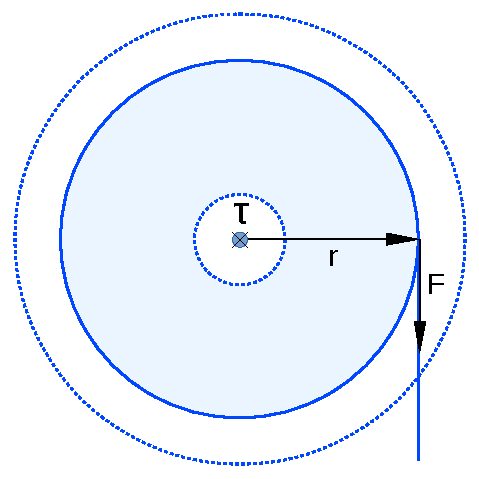
\includegraphics[height=2.5in]{figs/paper_roll2.pdf}}
\caption{Diagram of a roll of toilet paper, showing a force, lever arm, and the resulting torque.}
\label{paper_roll2}
\end{figure}

Figure~\ref{paper_roll2} shows the paper roll with $r$, $F$, and $\tau$.  As a vector quantity, the direction of $\tau$ is into the page, but we only care about its magnitude for now.


\section{Moment of inertia}

In the same way that linear acceleration is related to force by Newton's second law of motion, $F=ma$, angular acceleration is related to torque by another form of Newton's law:
%
\[ \tau = I \alpha \]
%
Where $\alpha$ is angular acceleration and $I$ is {\bf moment of inertia}.  Just as mass is what makes it harder to accelerate an object\footnote{That might sound like a dumb way to describe mass, but its actually one of the fundamental definitions.}, moment of inertia is what makes it harder to spin an object.
\index{mass}
\index{moment of inertia}

In the most general case, a 3-D object rotating around an arbitrary axis, moment of inertia is a tensor, which is a function that takes a vector as a parameter and returns a vector as a result.
\index{tensor}

Fortunately, in a system where all rotation and torque happens around a single axis, we don't have to deal with the most general case.  We can treat moment of inertia as a scalar quantity.
\index{scalar}

For a small point with mass $m$, rotating around a point at distance $r$, the moment of inertia is $I = m r^2$, in SI units \si{\kilogram\meter\squared}.  For more complex objects, we can compute $I$ by dividing the object into small masses, computing moments of inertia for each mass, and adding them up.

However, for most simple shapes, people have already done the calculations; you can just look up the answers.


\section{Unrolling}

Let's work on simulating the kitten unrolling the toilet paper.  Here's the \py{Condition} object with the parameters we'll need:
\index{Condition object}

\begin{python}
condition = Condition(Rmin = 0.02 * m,
                      Rmax = 0.055 * m,
                      L = 47 * m,
                      Mcore = 15e-3 * kg,
                      Mroll = 215e-3 * kg,
                      tension = 2e-4 * N,
                      duration = 180 * s)
\end{python}

As before, \py{Rmin} is the minimum radius and \py{Rmax} is the maximum.  \py{L} is the length of the paper.  \py{Mcore} is the mass of the cardboard tube at the center of the roll; \py{Mroll} is the mass of the paper.  \py{tension} is the force applied by the kitten, in \si{\newton}.  I chose a value that yields plausible results.

At \url{http://modsimpy.com/moment} you can find moments of inertia for simple geometric shapes.  I'll model the cardboard tube at the center of the roll as a ``thin cylindrical shell", and the paper roll as a ``thick-walled cylindrical tube with open ends".
\index{cylinder}

The moment of inertia for a thin shell is just $m r^2$, where $m$ is the mass and $r$ is the radius of the shell.

For a thick-walled tube the moment of inertia is
%
\[ I = \frac{\pi \rho h}{2} (r_2^4 - r_1^4) \]
%
where $\rho$ is the density of the material, $h$ is the height of the tube, $r_2$ is the outer diameter, and $r_1$ is the inner diameter.

Since the outer diameter changes as the kitten unrolls the paper, we have to compute the moment of inertia, at each point in time, as a function of the current radius, \py{r}.  Here's the function that does it:
\index{unpack}

\begin{python}
def moment_of_inertia(r, system):
    unpack(system)
    Icore = Mcore / 2 * Rmin**2
    Iroll = pi * rho_h / 2 * (r**4 - Rmin**4)
    return Icore + Iroll
\end{python}

\py{rho_h} is the product of density and height, $\rho h$, which is the mass per area.  \py{rho_h} is computed in \py{make_system}:
\index{density}
\index{\py{make_system}}

\begin{python}
def make_system(condition):
    unpack(condition)
    
    init = State(theta = 0 * radian,
                 omega = 0 * radian/s,
                 y = L)
    
    area = pi * (Rmax**2 - Rmin**2)
    rho_h = Mroll / area
    k = (Rmax**2 - Rmin**2) / 2 / L / radian    
    ts = linspace(0, duration, 101)
    
    return System(init=init, k=k, rho_h=rho_h,
                  Rmin=Rmin, Rmax=Rmax,
                  Mcore=Mcore, Mroll=Mroll, 
                  ts=ts)
\end{python}

\py{make_system} also computes \py{k}, using Equation~\ref{eqn4}.  Now we can write the slope function:
\index{slope function}
\index{function!slope}

\begin{python}
def slope_func(state, t, system):
    theta, omega, y = state
    unpack(system)
    
    r = sqrt(2*k*y + Rmin**2)
    I = moment_of_inertia(r, system)
    tau = r * tension
    alpha = tau / I
    dydt = -r * omega
    
    return omega, alpha, dydt
\end{python}

This slope function is similar to the previous one (Section~\ref{papersim}), with a few changes:

\begin{itemize}

\item \py{r} is no longer part of the \py{State} object.  Instead, we compute \py{r} at each time step, based on the current value of \py{y}, by Equation~\ref{eqn3}.
\index{time step}

\item Because \py{r} changes over time, we have to compute moment of inertia, \py{I}, at each time step\footnote{Actually, this is more of a problem than I have made it seem.  In the same way that $F = m a$ only applies when $m$ is constant, $\tau = I \alpha$ only applies when $I$ is constant.  When $I$ varies, we usually have to use a more general version of Newton's law.  However, in this example, mass and moment of inertia vary together in a way that makes the simple approach work out.}.

\item Angular velocity, \py{omega}, is no longer constant.  Instead, we compute torque, \py{tau}, and angular acceleration, \py{alpha}, at each time step.

\item I quietly changed the definition of \py{theta} so positive values of \py{theta} correspond to clockwise rotation, so \py{dydt = -r * omega}; that is, positive values of \py{omega} yield decreasing values of \py{y}, the amount of paper still on the roll.

\end{itemize} 

\py{slope_func} returns \py{omega}, \py{alpha}, and \py{dydt}, which are the derivatives of \py{theta}, \py{omega}, and \py{y}, respectively.

\begin{figure}[tb]
\centerline{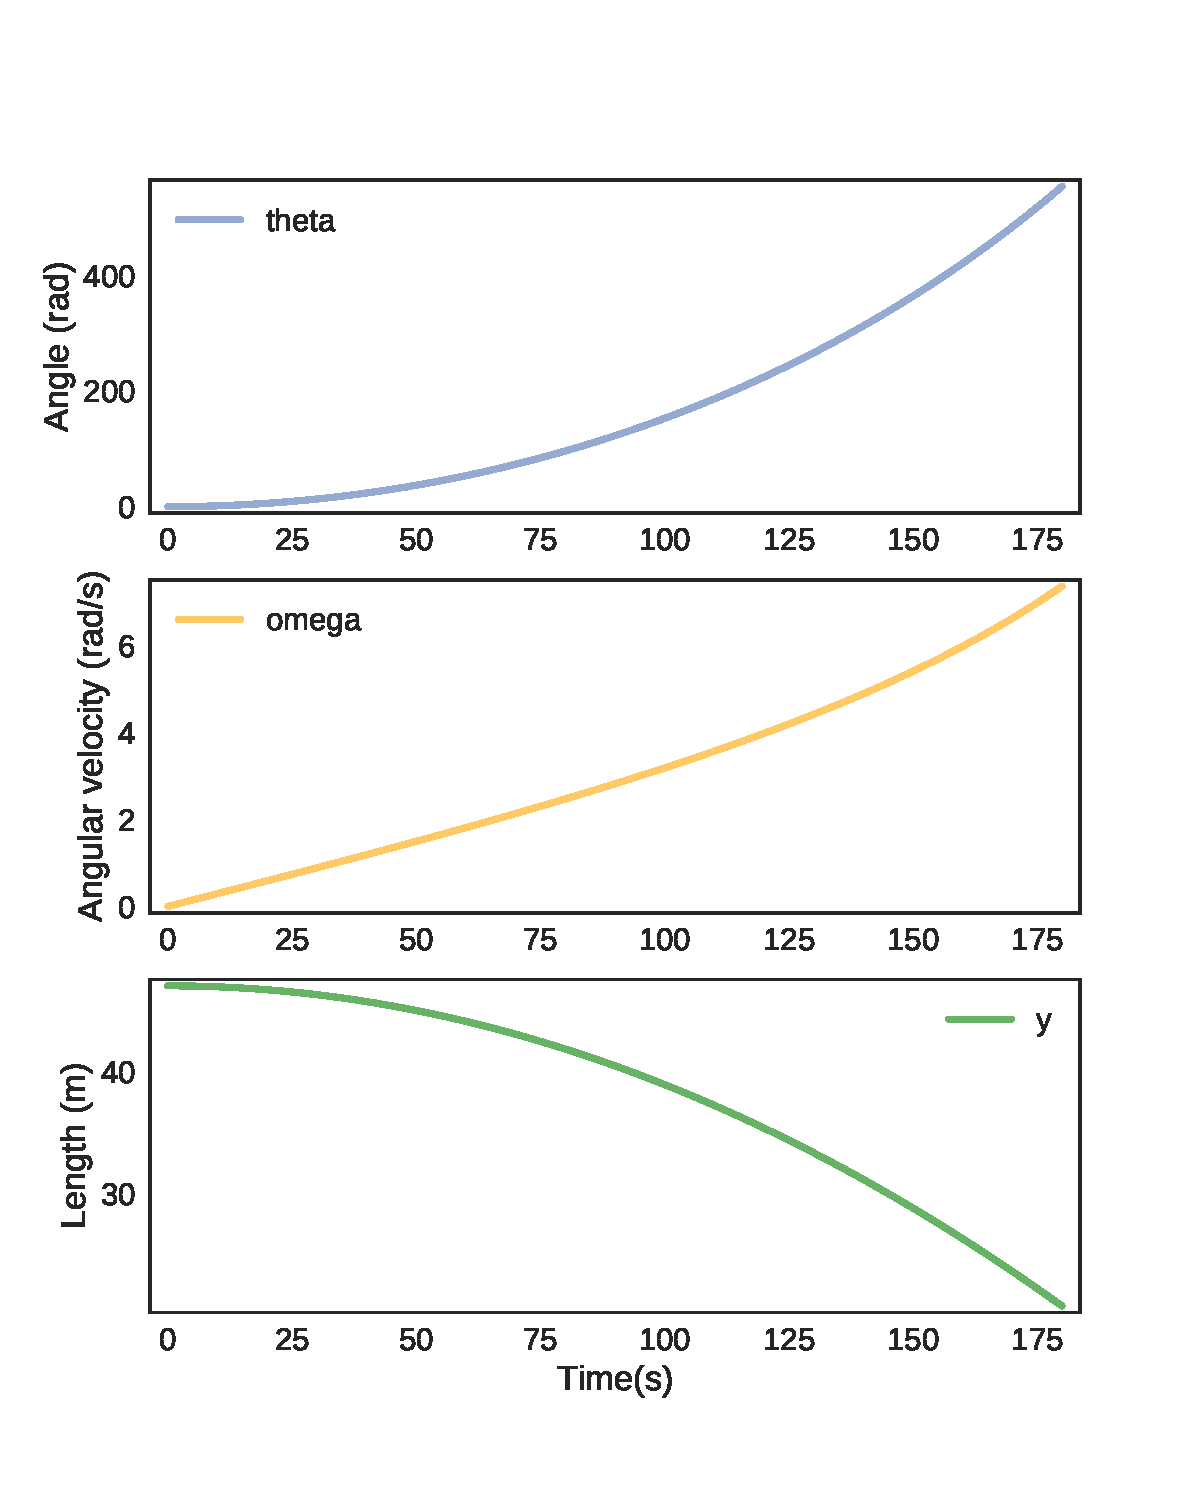
\includegraphics[width=3in]{figs/chap11-fig02.pdf}}
\caption{Simulation results showing rotation, angular velocity, and length over time.}
\label{chap11-fig02}
\end{figure}

Now we're ready to run the simulation.  Figure~\ref{chap11-fig02} shows the results.  Again, we can check the results to see if they seem plausible:

\begin{itemize}

\item Angular velocity, \py{omega}, increases almost linearly at first, as constant force yields almost constant torque.  Then, as the radius decreases, the lever arm decreases, yielding lower torque, but moment of inertia decreases even more, yielding higher angular acceleration.
\index{angular velocity}

\item The final value of \py{omega} is \SI{7.4}{\radian\per\second}, which is close to one revolution per second, so that seems plausible.

\item The final value of \py{theta} is \SI{555}{\radian}, which is about  
88 revolutions.  

\item The final value of \py{y} is \SI{21}{\meter} of paper left on the roll, which means the kitten pulled off \SI{26}{\meter} in two minutes.  That doesn't seem impossible, although it is based on a level of consistency and focus that is unlikely in a kitten.
\index{kitten}

\end{itemize}

This model yields results that seem reasonable, but remember that I chose the force applied by the kitten arbitrarily, and the model ignores friction between the paper roll and the axle.  This example is not meant to be particularly serious, but it is good preparation for the next problem, which is a little more interesting.


\section{Simulating a yo-yo}

Suppose you are holding a yo-yo with a length of string wound around its axle, and you drop it while holding the end of the string stationary.  As gravity accelerates the yo-yo downward, tension in the string exerts a force upward.  Since this force acts on a point offset from the center of mass, it exerts a torque that causes the yo-yo to spin.
\index{yo-yo}
\index{torque}
\index{lever arm}

\begin{figure}
\centerline{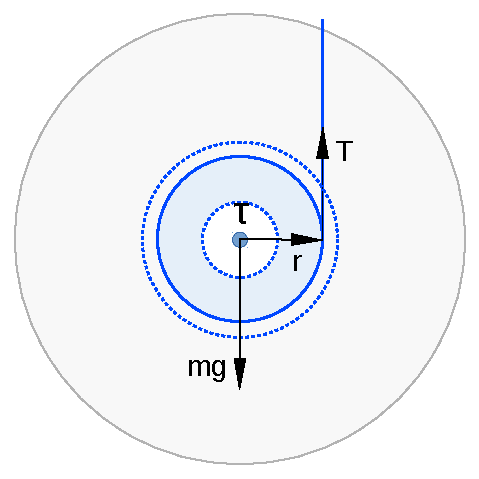
\includegraphics[height=2.5in]{figs/yoyo.pdf}}
\caption{Diagram of a yo-yo showing forces due to gravity and tension in the string, the lever arm of tension, and the resulting torque.}
\label{yoyo}
\end{figure}

Figure~\ref{yoyo} is a diagram of the forces on the yo-yo and the resulting torque.  The outer shaded area shows the body of the yo-yo.  The inner shaded area shows the rolled up string, the radius of which changes as the yo-yo unrolls.
\index{system of equations}

In this model, we can't figure out the linear and angular acceleration independently; we have to solve a system of equations:
%
\begin{align*}
\sum F &= m a \\
\sum \tau &= I \alpha
\end{align*}
%
where the summations indicate that we are adding up forces and torques.

As in the previous examples, linear and angular velocity are related because of the way the string unrolls:
%
\[ \frac{dy}{dt} = -r \frac{d \theta}{dt} \]
%
In this example, the linear and angular accelerations have opposite sign.  As the yo-yo rotates counter-clockwise, $\theta$ increases and $y$, which is the length of the rolled part of the string, decreases.

Taking the derivative of both sides yields a similar relationship between linear and angular acceleration:
%
\[ \frac{d^2 y}{dt^2} = -r \frac{d^2 \theta}{dt^2} \]
%
Which we can write more concisely:
%
\[ a = -r \alpha \]
%
This relationship is not a general law of nature; it is specific to scenarios like this where there is rolling without stretching or slipping.
\index{rolling}

Because of the way we've set up the problem, $y$ actually has two meanings: it represents the length of the rolled string and the height of the yo-yo, which decreases as the yo-yo falls.  Similarly, $a$ represents acceleration in the length of the rolled string and the height of the yo-yo.

We can compute the acceleration of the yo-yo by adding up the linear forces:
%
\[ \sum F = T - mg = ma \]
%
Where $T$ is positive because the tension force points up, and $mg$ is negative because gravity points down.

Because gravity acts on the center of mass, it creates no torque, so the only torque is due to tension:
%
\[ \sum \tau = T r = I \alpha \]
%
Positive (upward) tension yields positive (counter-clockwise) angular acceleration.
\index{SymPy}

Now we have three equations in three unknowns, $T$, $a$, and $\alpha$, with $I$, $m$, $g$, and $r$ as known quantities.  It is simple enough to solve these equations by hand, but we can also get SymPy to do it for us:

\begin{python}
T, a, alpha, I, m, g, r = symbols('T a alpha I m g r')
eq1 = Eq(a, -r * alpha)
eq2 = Eq(T - m*g, m * a)
eq3 = Eq(T * r, I * alpha)
soln = solve([eq1, eq2, eq3], [T, a, alpha])
\end{python}

The results are
%
\begin{align*}
T      &= m g I / I^*   \\
a      &= -m g r^2 / I^* \\
\alpha &= m g r / I^*    \\
\end{align*}
%
where $I^*$ is the augmented moment of inertia, $I + m r^2$.

To simulate the system, we don't really need $T$; we can plug $a$ and $\alpha$ directly into the slope function.

At this point you have everything you need to simulate the descent of a yo-yo.  In the notebook for this chapter you will have a chance to finish off the exercise.


\chapter{Second order systems}

% Pendulum:

% Springy pendulum

% Stiff problem as k increases

% Add drag

% Rigid pendulum: solve those constraints

% Generalized coordinates


\backmatter
\printindex

\afterpage{\blankpage}


\end{document}

\end{itemize}
